\documentclass[twoside]{book}

% Packages required by doxygen
\usepackage{fixltx2e}
\usepackage{calc}
\usepackage{doxygen}
\usepackage[export]{adjustbox} % also loads graphicx
\usepackage{graphicx}
\usepackage[utf8]{inputenc}
\usepackage{makeidx}
\usepackage{multicol}
\usepackage{multirow}
\PassOptionsToPackage{warn}{textcomp}
\usepackage{textcomp}
\usepackage[nointegrals]{wasysym}
\usepackage[table]{xcolor}

% Font selection
\usepackage[T1]{fontenc}
\usepackage[scaled=.90]{helvet}
\usepackage{courier}
\usepackage{amssymb}
\usepackage{sectsty}
\renewcommand{\familydefault}{\sfdefault}
\allsectionsfont{%
  \fontseries{bc}\selectfont%
  \color{darkgray}%
}
\renewcommand{\DoxyLabelFont}{%
  \fontseries{bc}\selectfont%
  \color{darkgray}%
}
\newcommand{\+}{\discretionary{\mbox{\scriptsize$\hookleftarrow$}}{}{}}

% Page & text layout
\usepackage{geometry}
\geometry{%
  a4paper,%
  top=2.5cm,%
  bottom=2.5cm,%
  left=2.5cm,%
  right=2.5cm%
}
\tolerance=750
\hfuzz=15pt
\hbadness=750
\setlength{\emergencystretch}{15pt}
\setlength{\parindent}{0cm}
\setlength{\parskip}{0.2cm}
\makeatletter
\renewcommand{\paragraph}{%
  \@startsection{paragraph}{4}{0ex}{-1.0ex}{1.0ex}{%
    \normalfont\normalsize\bfseries\SS@parafont%
  }%
}
\renewcommand{\subparagraph}{%
  \@startsection{subparagraph}{5}{0ex}{-1.0ex}{1.0ex}{%
    \normalfont\normalsize\bfseries\SS@subparafont%
  }%
}
\makeatother

% Headers & footers
\usepackage{fancyhdr}
\pagestyle{fancyplain}
\fancyhead[LE]{\fancyplain{}{\bfseries\thepage}}
\fancyhead[CE]{\fancyplain{}{}}
\fancyhead[RE]{\fancyplain{}{\bfseries\leftmark}}
\fancyhead[LO]{\fancyplain{}{\bfseries\rightmark}}
\fancyhead[CO]{\fancyplain{}{}}
\fancyhead[RO]{\fancyplain{}{\bfseries\thepage}}
\fancyfoot[LE]{\fancyplain{}{}}
\fancyfoot[CE]{\fancyplain{}{}}
\fancyfoot[RE]{\fancyplain{}{\bfseries\scriptsize Generated on Sat Sep 5 2015 18\+:26\+:48 for F\+T\+C\+Android\+Library by Doxygen }}
\fancyfoot[LO]{\fancyplain{}{\bfseries\scriptsize Generated on Sat Sep 5 2015 18\+:26\+:48 for F\+T\+C\+Android\+Library by Doxygen }}
\fancyfoot[CO]{\fancyplain{}{}}
\fancyfoot[RO]{\fancyplain{}{}}
\renewcommand{\footrulewidth}{0.4pt}
\renewcommand{\chaptermark}[1]{%
  \markboth{#1}{}%
}
\renewcommand{\sectionmark}[1]{%
  \markright{\thesection\ #1}%
}

% Indices & bibliography
\usepackage{natbib}
\usepackage[titles]{tocloft}
\setcounter{tocdepth}{3}
\setcounter{secnumdepth}{5}
\makeindex

% Hyperlinks (required, but should be loaded last)
\usepackage{ifpdf}
\ifpdf
  \usepackage[pdftex,pagebackref=true]{hyperref}
\else
  \usepackage[ps2pdf,pagebackref=true]{hyperref}
\fi
\hypersetup{%
  colorlinks=true,%
  linkcolor=blue,%
  citecolor=blue,%
  unicode%
}

% Custom commands
\newcommand{\clearemptydoublepage}{%
  \newpage{\pagestyle{empty}\cleardoublepage}%
}


%===== C O N T E N T S =====

\begin{document}

% Titlepage & ToC
\hypersetup{pageanchor=false,
             bookmarks=true,
             bookmarksnumbered=true,
             pdfencoding=unicode
            }
\pagenumbering{roman}
\begin{titlepage}
\vspace*{7cm}
\begin{center}%
{\Large F\+T\+C\+Android\+Library }\\
\vspace*{1cm}
{\large Generated by Doxygen 1.8.10}\\
\vspace*{0.5cm}
{\small Sat Sep 5 2015 18:26:48}\\
\end{center}
\end{titlepage}
\clearemptydoublepage
\tableofcontents
\clearemptydoublepage
\pagenumbering{arabic}
\hypersetup{pageanchor=true}

%--- Begin generated contents ---
\chapter{Hierarchical Index}
\section{Class Hierarchy}
This inheritance list is sorted roughly, but not completely, alphabetically\+:\begin{DoxyCompactList}
\item \contentsline{section}{com.\+lasarobotics.\+library.\+doodle.\+actions.\+Action}{\pageref{classcom_1_1lasarobotics_1_1library_1_1doodle_1_1actions_1_1_action}}{}
\begin{DoxyCompactList}
\item \contentsline{section}{com.\+lasarobotics.\+library.\+doodle.\+actions.\+Motor\+Move}{\pageref{classcom_1_1lasarobotics_1_1library_1_1doodle_1_1actions_1_1_motor_move}}{}
\item \contentsline{section}{com.\+lasarobotics.\+library.\+doodle.\+actions.\+No\+Operation}{\pageref{classcom_1_1lasarobotics_1_1library_1_1doodle_1_1actions_1_1_no_operation}}{}
\item \contentsline{section}{com.\+lasarobotics.\+library.\+doodle.\+actions.\+wait.\+Wait\+Forever}{\pageref{classcom_1_1lasarobotics_1_1library_1_1doodle_1_1actions_1_1wait_1_1_wait_forever}}{}
\item \contentsline{section}{com.\+lasarobotics.\+library.\+doodle.\+actions.\+wait.\+Wait\+Time}{\pageref{classcom_1_1lasarobotics_1_1library_1_1doodle_1_1actions_1_1wait_1_1_wait_time}}{}
\end{DoxyCompactList}
\item \contentsline{section}{com.\+lasarobotics.\+library.\+controller.\+Button\+State}{\pageref{classcom_1_1lasarobotics_1_1library_1_1controller_1_1_button_state}}{}
\item \contentsline{section}{com.\+lasarobotics.\+library.\+util.\+Constants}{\pageref{classcom_1_1lasarobotics_1_1library_1_1util_1_1_constants}}{}
\item \contentsline{section}{com.\+lasarobotics.\+library.\+controller.\+Controller}{\pageref{classcom_1_1lasarobotics_1_1library_1_1controller_1_1_controller}}{}
\item \contentsline{section}{com.\+lasarobotics.\+library.\+util.\+Distance\+Unit}{\pageref{enumcom_1_1lasarobotics_1_1library_1_1util_1_1_distance_unit}}{}
\item \contentsline{section}{com.\+lasarobotics.\+library.\+doodle.\+Doodle\+Do}{\pageref{classcom_1_1lasarobotics_1_1library_1_1doodle_1_1_doodle_do}}{}
\item \contentsline{section}{com.\+lasarobotics.\+library.\+doodle.\+Doodle\+Map}{\pageref{classcom_1_1lasarobotics_1_1library_1_1doodle_1_1_doodle_map}}{}
\item \contentsline{section}{com.\+lasarobotics.\+library.\+doodle.\+maps.\+Doodle\+Map}{\pageref{classcom_1_1lasarobotics_1_1library_1_1doodle_1_1maps_1_1_doodle_map}}{}
\item \contentsline{section}{com.\+lasarobotics.\+library.\+doodle.\+Doodle\+Run\+Data}{\pageref{classcom_1_1lasarobotics_1_1library_1_1doodle_1_1_doodle_run_data}}{}
\item \contentsline{section}{com.\+lasarobotics.\+library.\+doodle.\+Doodle\+Write}{\pageref{classcom_1_1lasarobotics_1_1library_1_1doodle_1_1_doodle_write}}{}
\item \contentsline{section}{com.\+lasarobotics.\+library.\+sensor.\+legacy.\+hitechnic.\+Gyroscope}{\pageref{classcom_1_1lasarobotics_1_1library_1_1sensor_1_1legacy_1_1hitechnic_1_1_gyroscope}}{}
\item \contentsline{section}{com.\+lasarobotics.\+library.\+sensor.\+generic.\+I\+R}{\pageref{classcom_1_1lasarobotics_1_1library_1_1sensor_1_1generic_1_1_i_r}}{}
\item \contentsline{section}{com.\+lasarobotics.\+library.\+skynet.\+Kalman}{\pageref{classcom_1_1lasarobotics_1_1library_1_1skynet_1_1_kalman}}{}
\item \contentsline{section}{com.\+lasarobotics.\+library.\+sensor.\+generic.\+Li\+D\+A\+R}{\pageref{classcom_1_1lasarobotics_1_1library_1_1sensor_1_1generic_1_1_li_d_a_r}}{}
\item \contentsline{section}{com.\+lasarobotics.\+library.\+util.\+Lookup\+Table$<$ T $>$}{\pageref{classcom_1_1lasarobotics_1_1library_1_1util_1_1_lookup_table}}{}
\item \contentsline{section}{com.\+lasarobotics.\+library.\+util.\+Math\+Util}{\pageref{classcom_1_1lasarobotics_1_1library_1_1util_1_1_math_util}}{}
\item \contentsline{section}{com.\+lasarobotics.\+library.\+drive.\+Mecanum}{\pageref{classcom_1_1lasarobotics_1_1library_1_1drive_1_1_mecanum}}{}
\item \contentsline{section}{com.\+lasarobotics.\+library.\+monkeyc.\+Monkey\+C}{\pageref{classcom_1_1lasarobotics_1_1library_1_1monkeyc_1_1_monkey_c}}{}
\item \contentsline{section}{com.\+lasarobotics.\+library.\+monkeyc.\+Monkey\+Data}{\pageref{classcom_1_1lasarobotics_1_1library_1_1monkeyc_1_1_monkey_data}}{}
\item \contentsline{section}{com.\+lasarobotics.\+library.\+monkeyc.\+Monkey\+Do}{\pageref{classcom_1_1lasarobotics_1_1library_1_1monkeyc_1_1_monkey_do}}{}
\item \contentsline{section}{com.\+lasarobotics.\+library.\+monkeyc.\+Monkey\+Util}{\pageref{classcom_1_1lasarobotics_1_1library_1_1monkeyc_1_1_monkey_util}}{}
\item \contentsline{section}{com.\+lasarobotics.\+library.\+doodle.\+actions.\+sensors.\+Motor\+Encoder\+Reset}{\pageref{classcom_1_1lasarobotics_1_1library_1_1doodle_1_1actions_1_1sensors_1_1_motor_encoder_reset}}{}
\item \contentsline{section}{com.\+lasarobotics.\+library.\+doodle.\+Doodle\+Map.\+Motor\+Flags}{\pageref{enumcom_1_1lasarobotics_1_1library_1_1doodle_1_1_doodle_map_1_1_motor_flags}}{}
\item \contentsline{section}{com.\+lasarobotics.\+library.\+sensor.\+modernrobotics.\+Optical\+Distance}{\pageref{classcom_1_1lasarobotics_1_1library_1_1sensor_1_1modernrobotics_1_1_optical_distance}}{}
\item \contentsline{section}{com.\+lasarobotics.\+library.\+doodle.\+maps.\+Doodle\+Map.\+Range\+Of\+Motion}{\pageref{enumcom_1_1lasarobotics_1_1library_1_1doodle_1_1maps_1_1_doodle_map_1_1_range_of_motion}}{}
\item \contentsline{section}{com.\+lasarobotics.\+library.\+util.\+Rolling\+Average$<$ T extends Number $>$}{\pageref{classcom_1_1lasarobotics_1_1library_1_1util_1_1_rolling_average}}{}
\item \contentsline{section}{com.\+lasarobotics.\+library.\+util.\+Rolling\+Average$<$ Double $>$}{\pageref{classcom_1_1lasarobotics_1_1library_1_1util_1_1_rolling_average}}{}
\item \contentsline{section}{com.\+lasarobotics.\+library.\+sensor.\+android.\+Sensors}{\pageref{classcom_1_1lasarobotics_1_1library_1_1sensor_1_1android_1_1_sensors}}{}
\item \contentsline{section}{com.\+lasarobotics.\+library.\+drive.\+Swerve}{\pageref{classcom_1_1lasarobotics_1_1library_1_1drive_1_1_swerve}}{}
\item \contentsline{section}{com.\+lasarobotics.\+library.\+drive.\+Tank}{\pageref{classcom_1_1lasarobotics_1_1library_1_1drive_1_1_tank}}{}
\item \contentsline{section}{com.\+lasarobotics.\+library.\+util.\+Timers}{\pageref{classcom_1_1lasarobotics_1_1library_1_1util_1_1_timers}}{}
\item \contentsline{section}{com.\+lasarobotics.\+library.\+sensor.\+legacy.\+lego.\+Touch}{\pageref{classcom_1_1lasarobotics_1_1library_1_1sensor_1_1legacy_1_1lego_1_1_touch}}{}
\item \contentsline{section}{com.\+lasarobotics.\+library.\+sensor.\+modernrobotics.\+Touch}{\pageref{classcom_1_1lasarobotics_1_1library_1_1sensor_1_1modernrobotics_1_1_touch}}{}
\item \contentsline{section}{com.\+lasarobotics.\+library.\+sensor.\+legacy.\+lego.\+Ultrasonic}{\pageref{classcom_1_1lasarobotics_1_1library_1_1sensor_1_1legacy_1_1lego_1_1_ultrasonic}}{}
\item \contentsline{section}{com.\+lasarobotics.\+library.\+android.\+Util}{\pageref{classcom_1_1lasarobotics_1_1library_1_1android_1_1_util}}{}
\item \contentsline{section}{com.\+lasarobotics.\+library.\+util.\+Vector3$<$ T $>$}{\pageref{classcom_1_1lasarobotics_1_1library_1_1util_1_1_vector3}}{}
\item \contentsline{section}{com.\+lasarobotics.\+library.\+sensor.\+modernrobotics.\+Voltage}{\pageref{classcom_1_1lasarobotics_1_1library_1_1sensor_1_1modernrobotics_1_1_voltage}}{}
\item Sensor\+Event\+Listener\begin{DoxyCompactList}
\item \contentsline{section}{com.\+lasarobotics.\+library.\+sensor.\+android.\+Linear\+Acceleration}{\pageref{classcom_1_1lasarobotics_1_1library_1_1sensor_1_1android_1_1_linear_acceleration}}{}
\end{DoxyCompactList}
\item Touch\+Sensor\end{DoxyCompactList}

\chapter{Class Index}
\section{Class List}
Here are the classes, structs, unions and interfaces with brief descriptions\+:\begin{DoxyCompactList}
\item\contentsline{section}{\hyperlink{classcom_1_1lasarobotics_1_1library_1_1doodle_1_1actions_1_1_action}{com.\+lasarobotics.\+library.\+doodle.\+actions.\+Action} }{\pageref{classcom_1_1lasarobotics_1_1library_1_1doodle_1_1actions_1_1_action}}{}
\item\contentsline{section}{\hyperlink{classcom_1_1lasarobotics_1_1library_1_1controller_1_1_button_state}{com.\+lasarobotics.\+library.\+controller.\+Button\+State} }{\pageref{classcom_1_1lasarobotics_1_1library_1_1controller_1_1_button_state}}{}
\item\contentsline{section}{\hyperlink{classcom_1_1lasarobotics_1_1library_1_1util_1_1_constants}{com.\+lasarobotics.\+library.\+util.\+Constants} }{\pageref{classcom_1_1lasarobotics_1_1library_1_1util_1_1_constants}}{}
\item\contentsline{section}{\hyperlink{classcom_1_1lasarobotics_1_1library_1_1controller_1_1_controller}{com.\+lasarobotics.\+library.\+controller.\+Controller} }{\pageref{classcom_1_1lasarobotics_1_1library_1_1controller_1_1_controller}}{}
\item\contentsline{section}{\hyperlink{enumcom_1_1lasarobotics_1_1library_1_1util_1_1_distance_unit}{com.\+lasarobotics.\+library.\+util.\+Distance\+Unit} }{\pageref{enumcom_1_1lasarobotics_1_1library_1_1util_1_1_distance_unit}}{}
\item\contentsline{section}{\hyperlink{classcom_1_1lasarobotics_1_1library_1_1doodle_1_1_doodle_do}{com.\+lasarobotics.\+library.\+doodle.\+Doodle\+Do} }{\pageref{classcom_1_1lasarobotics_1_1library_1_1doodle_1_1_doodle_do}}{}
\item\contentsline{section}{\hyperlink{classcom_1_1lasarobotics_1_1library_1_1doodle_1_1_doodle_map}{com.\+lasarobotics.\+library.\+doodle.\+Doodle\+Map} }{\pageref{classcom_1_1lasarobotics_1_1library_1_1doodle_1_1_doodle_map}}{}
\item\contentsline{section}{\hyperlink{classcom_1_1lasarobotics_1_1library_1_1doodle_1_1maps_1_1_doodle_map}{com.\+lasarobotics.\+library.\+doodle.\+maps.\+Doodle\+Map} }{\pageref{classcom_1_1lasarobotics_1_1library_1_1doodle_1_1maps_1_1_doodle_map}}{}
\item\contentsline{section}{\hyperlink{classcom_1_1lasarobotics_1_1library_1_1doodle_1_1_doodle_run_data}{com.\+lasarobotics.\+library.\+doodle.\+Doodle\+Run\+Data} }{\pageref{classcom_1_1lasarobotics_1_1library_1_1doodle_1_1_doodle_run_data}}{}
\item\contentsline{section}{\hyperlink{classcom_1_1lasarobotics_1_1library_1_1doodle_1_1_doodle_write}{com.\+lasarobotics.\+library.\+doodle.\+Doodle\+Write} }{\pageref{classcom_1_1lasarobotics_1_1library_1_1doodle_1_1_doodle_write}}{}
\item\contentsline{section}{\hyperlink{classcom_1_1lasarobotics_1_1library_1_1sensor_1_1legacy_1_1hitechnic_1_1_gyroscope}{com.\+lasarobotics.\+library.\+sensor.\+legacy.\+hitechnic.\+Gyroscope} }{\pageref{classcom_1_1lasarobotics_1_1library_1_1sensor_1_1legacy_1_1hitechnic_1_1_gyroscope}}{}
\item\contentsline{section}{\hyperlink{classcom_1_1lasarobotics_1_1library_1_1sensor_1_1generic_1_1_i_r}{com.\+lasarobotics.\+library.\+sensor.\+generic.\+I\+R} }{\pageref{classcom_1_1lasarobotics_1_1library_1_1sensor_1_1generic_1_1_i_r}}{}
\item\contentsline{section}{\hyperlink{classcom_1_1lasarobotics_1_1library_1_1skynet_1_1_kalman}{com.\+lasarobotics.\+library.\+skynet.\+Kalman} }{\pageref{classcom_1_1lasarobotics_1_1library_1_1skynet_1_1_kalman}}{}
\item\contentsline{section}{\hyperlink{classcom_1_1lasarobotics_1_1library_1_1sensor_1_1generic_1_1_li_d_a_r}{com.\+lasarobotics.\+library.\+sensor.\+generic.\+Li\+D\+A\+R} }{\pageref{classcom_1_1lasarobotics_1_1library_1_1sensor_1_1generic_1_1_li_d_a_r}}{}
\item\contentsline{section}{\hyperlink{classcom_1_1lasarobotics_1_1library_1_1sensor_1_1android_1_1_linear_acceleration}{com.\+lasarobotics.\+library.\+sensor.\+android.\+Linear\+Acceleration} }{\pageref{classcom_1_1lasarobotics_1_1library_1_1sensor_1_1android_1_1_linear_acceleration}}{}
\item\contentsline{section}{\hyperlink{classcom_1_1lasarobotics_1_1library_1_1util_1_1_lookup_table}{com.\+lasarobotics.\+library.\+util.\+Lookup\+Table$<$ T $>$} }{\pageref{classcom_1_1lasarobotics_1_1library_1_1util_1_1_lookup_table}}{}
\item\contentsline{section}{\hyperlink{classcom_1_1lasarobotics_1_1library_1_1util_1_1_math_util}{com.\+lasarobotics.\+library.\+util.\+Math\+Util} }{\pageref{classcom_1_1lasarobotics_1_1library_1_1util_1_1_math_util}}{}
\item\contentsline{section}{\hyperlink{classcom_1_1lasarobotics_1_1library_1_1drive_1_1_mecanum}{com.\+lasarobotics.\+library.\+drive.\+Mecanum} }{\pageref{classcom_1_1lasarobotics_1_1library_1_1drive_1_1_mecanum}}{}
\item\contentsline{section}{\hyperlink{classcom_1_1lasarobotics_1_1library_1_1monkeyc_1_1_monkey_c}{com.\+lasarobotics.\+library.\+monkeyc.\+Monkey\+C} }{\pageref{classcom_1_1lasarobotics_1_1library_1_1monkeyc_1_1_monkey_c}}{}
\item\contentsline{section}{\hyperlink{classcom_1_1lasarobotics_1_1library_1_1monkeyc_1_1_monkey_data}{com.\+lasarobotics.\+library.\+monkeyc.\+Monkey\+Data} }{\pageref{classcom_1_1lasarobotics_1_1library_1_1monkeyc_1_1_monkey_data}}{}
\item\contentsline{section}{\hyperlink{classcom_1_1lasarobotics_1_1library_1_1monkeyc_1_1_monkey_do}{com.\+lasarobotics.\+library.\+monkeyc.\+Monkey\+Do} }{\pageref{classcom_1_1lasarobotics_1_1library_1_1monkeyc_1_1_monkey_do}}{}
\item\contentsline{section}{\hyperlink{classcom_1_1lasarobotics_1_1library_1_1monkeyc_1_1_monkey_util}{com.\+lasarobotics.\+library.\+monkeyc.\+Monkey\+Util} }{\pageref{classcom_1_1lasarobotics_1_1library_1_1monkeyc_1_1_monkey_util}}{}
\item\contentsline{section}{\hyperlink{classcom_1_1lasarobotics_1_1library_1_1doodle_1_1actions_1_1sensors_1_1_motor_encoder_reset}{com.\+lasarobotics.\+library.\+doodle.\+actions.\+sensors.\+Motor\+Encoder\+Reset} }{\pageref{classcom_1_1lasarobotics_1_1library_1_1doodle_1_1actions_1_1sensors_1_1_motor_encoder_reset}}{}
\item\contentsline{section}{\hyperlink{enumcom_1_1lasarobotics_1_1library_1_1doodle_1_1_doodle_map_1_1_motor_flags}{com.\+lasarobotics.\+library.\+doodle.\+Doodle\+Map.\+Motor\+Flags} }{\pageref{enumcom_1_1lasarobotics_1_1library_1_1doodle_1_1_doodle_map_1_1_motor_flags}}{}
\item\contentsline{section}{\hyperlink{classcom_1_1lasarobotics_1_1library_1_1doodle_1_1actions_1_1_motor_move}{com.\+lasarobotics.\+library.\+doodle.\+actions.\+Motor\+Move} }{\pageref{classcom_1_1lasarobotics_1_1library_1_1doodle_1_1actions_1_1_motor_move}}{}
\item\contentsline{section}{\hyperlink{classcom_1_1lasarobotics_1_1library_1_1doodle_1_1actions_1_1_no_operation}{com.\+lasarobotics.\+library.\+doodle.\+actions.\+No\+Operation} }{\pageref{classcom_1_1lasarobotics_1_1library_1_1doodle_1_1actions_1_1_no_operation}}{}
\item\contentsline{section}{\hyperlink{classcom_1_1lasarobotics_1_1library_1_1sensor_1_1modernrobotics_1_1_optical_distance}{com.\+lasarobotics.\+library.\+sensor.\+modernrobotics.\+Optical\+Distance} }{\pageref{classcom_1_1lasarobotics_1_1library_1_1sensor_1_1modernrobotics_1_1_optical_distance}}{}
\item\contentsline{section}{\hyperlink{enumcom_1_1lasarobotics_1_1library_1_1doodle_1_1maps_1_1_doodle_map_1_1_range_of_motion}{com.\+lasarobotics.\+library.\+doodle.\+maps.\+Doodle\+Map.\+Range\+Of\+Motion} }{\pageref{enumcom_1_1lasarobotics_1_1library_1_1doodle_1_1maps_1_1_doodle_map_1_1_range_of_motion}}{}
\item\contentsline{section}{\hyperlink{classcom_1_1lasarobotics_1_1library_1_1util_1_1_rolling_average}{com.\+lasarobotics.\+library.\+util.\+Rolling\+Average$<$ T extends Number $>$} }{\pageref{classcom_1_1lasarobotics_1_1library_1_1util_1_1_rolling_average}}{}
\item\contentsline{section}{\hyperlink{classcom_1_1lasarobotics_1_1library_1_1sensor_1_1android_1_1_sensors}{com.\+lasarobotics.\+library.\+sensor.\+android.\+Sensors} }{\pageref{classcom_1_1lasarobotics_1_1library_1_1sensor_1_1android_1_1_sensors}}{}
\item\contentsline{section}{\hyperlink{classcom_1_1lasarobotics_1_1library_1_1drive_1_1_swerve}{com.\+lasarobotics.\+library.\+drive.\+Swerve} }{\pageref{classcom_1_1lasarobotics_1_1library_1_1drive_1_1_swerve}}{}
\item\contentsline{section}{\hyperlink{classcom_1_1lasarobotics_1_1library_1_1drive_1_1_tank}{com.\+lasarobotics.\+library.\+drive.\+Tank} }{\pageref{classcom_1_1lasarobotics_1_1library_1_1drive_1_1_tank}}{}
\item\contentsline{section}{\hyperlink{classcom_1_1lasarobotics_1_1library_1_1util_1_1_timers}{com.\+lasarobotics.\+library.\+util.\+Timers} }{\pageref{classcom_1_1lasarobotics_1_1library_1_1util_1_1_timers}}{}
\item\contentsline{section}{\hyperlink{classcom_1_1lasarobotics_1_1library_1_1sensor_1_1legacy_1_1lego_1_1_touch}{com.\+lasarobotics.\+library.\+sensor.\+legacy.\+lego.\+Touch} }{\pageref{classcom_1_1lasarobotics_1_1library_1_1sensor_1_1legacy_1_1lego_1_1_touch}}{}
\item\contentsline{section}{\hyperlink{classcom_1_1lasarobotics_1_1library_1_1sensor_1_1modernrobotics_1_1_touch}{com.\+lasarobotics.\+library.\+sensor.\+modernrobotics.\+Touch} }{\pageref{classcom_1_1lasarobotics_1_1library_1_1sensor_1_1modernrobotics_1_1_touch}}{}
\item\contentsline{section}{\hyperlink{classcom_1_1lasarobotics_1_1library_1_1sensor_1_1legacy_1_1lego_1_1_ultrasonic}{com.\+lasarobotics.\+library.\+sensor.\+legacy.\+lego.\+Ultrasonic} }{\pageref{classcom_1_1lasarobotics_1_1library_1_1sensor_1_1legacy_1_1lego_1_1_ultrasonic}}{}
\item\contentsline{section}{\hyperlink{classcom_1_1lasarobotics_1_1library_1_1android_1_1_util}{com.\+lasarobotics.\+library.\+android.\+Util} }{\pageref{classcom_1_1lasarobotics_1_1library_1_1android_1_1_util}}{}
\item\contentsline{section}{\hyperlink{classcom_1_1lasarobotics_1_1library_1_1util_1_1_vector3}{com.\+lasarobotics.\+library.\+util.\+Vector3$<$ T $>$} }{\pageref{classcom_1_1lasarobotics_1_1library_1_1util_1_1_vector3}}{}
\item\contentsline{section}{\hyperlink{classcom_1_1lasarobotics_1_1library_1_1sensor_1_1modernrobotics_1_1_voltage}{com.\+lasarobotics.\+library.\+sensor.\+modernrobotics.\+Voltage} }{\pageref{classcom_1_1lasarobotics_1_1library_1_1sensor_1_1modernrobotics_1_1_voltage}}{}
\item\contentsline{section}{\hyperlink{classcom_1_1lasarobotics_1_1library_1_1doodle_1_1actions_1_1wait_1_1_wait_forever}{com.\+lasarobotics.\+library.\+doodle.\+actions.\+wait.\+Wait\+Forever} }{\pageref{classcom_1_1lasarobotics_1_1library_1_1doodle_1_1actions_1_1wait_1_1_wait_forever}}{}
\item\contentsline{section}{\hyperlink{classcom_1_1lasarobotics_1_1library_1_1doodle_1_1actions_1_1wait_1_1_wait_time}{com.\+lasarobotics.\+library.\+doodle.\+actions.\+wait.\+Wait\+Time} }{\pageref{classcom_1_1lasarobotics_1_1library_1_1doodle_1_1actions_1_1wait_1_1_wait_time}}{}
\end{DoxyCompactList}

\chapter{Class Documentation}
\hypertarget{classcom_1_1lasarobotics_1_1library_1_1doodle_1_1actions_1_1_action}{}\section{com.\+lasarobotics.\+library.\+doodle.\+actions.\+Action Class Reference}
\label{classcom_1_1lasarobotics_1_1library_1_1doodle_1_1actions_1_1_action}\index{com.\+lasarobotics.\+library.\+doodle.\+actions.\+Action@{com.\+lasarobotics.\+library.\+doodle.\+actions.\+Action}}
Inheritance diagram for com.\+lasarobotics.\+library.\+doodle.\+actions.\+Action\+:\begin{figure}[H]
\begin{center}
\leavevmode
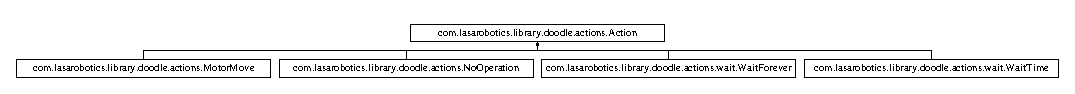
\includegraphics[height=0.818713cm]{classcom_1_1lasarobotics_1_1library_1_1doodle_1_1actions_1_1_action}
\end{center}
\end{figure}
\subsection*{Public Member Functions}
\begin{DoxyCompactItemize}
\item 
\hypertarget{classcom_1_1lasarobotics_1_1library_1_1doodle_1_1actions_1_1_action_a29325ad8bfd4c26adaebb485f22db577}{}abstract void {\bfseries run} (\hyperlink{classcom_1_1lasarobotics_1_1library_1_1doodle_1_1_doodle_run_data}{Doodle\+Run\+Data} data)\label{classcom_1_1lasarobotics_1_1library_1_1doodle_1_1actions_1_1_action_a29325ad8bfd4c26adaebb485f22db577}

\item 
\hypertarget{classcom_1_1lasarobotics_1_1library_1_1doodle_1_1actions_1_1_action_a2310b2bb2e4557f7e7d2a7d92fd563c3}{}abstract String {\bfseries to\+String} ()\label{classcom_1_1lasarobotics_1_1library_1_1doodle_1_1actions_1_1_action_a2310b2bb2e4557f7e7d2a7d92fd563c3}

\end{DoxyCompactItemize}
\subsection*{Protected Member Functions}
\begin{DoxyCompactItemize}
\item 
\hypertarget{classcom_1_1lasarobotics_1_1library_1_1doodle_1_1actions_1_1_action_a8973bac07f54daedf9229a8d43dde042}{}{\bfseries Action} (String name)\label{classcom_1_1lasarobotics_1_1library_1_1doodle_1_1actions_1_1_action_a8973bac07f54daedf9229a8d43dde042}

\end{DoxyCompactItemize}


\subsection{Detailed Description}
Defines a custom robot action These actions are stored in the same file as the instruction data 

The documentation for this class was generated from the following file\+:\begin{DoxyCompactItemize}
\item 
ftc-\/library/src/main/java/com/lasarobotics/library/doodle/actions/Action.\+java\end{DoxyCompactItemize}

\hypertarget{classcom_1_1lasarobotics_1_1library_1_1controller_1_1_button_state}{}\section{com.\+lasarobotics.\+library.\+controller.\+Button\+State Class Reference}
\label{classcom_1_1lasarobotics_1_1library_1_1controller_1_1_button_state}\index{com.\+lasarobotics.\+library.\+controller.\+Button\+State@{com.\+lasarobotics.\+library.\+controller.\+Button\+State}}
\subsection*{Static Public Attributes}
\begin{DoxyCompactItemize}
\item 
\hypertarget{classcom_1_1lasarobotics_1_1library_1_1controller_1_1_button_state_a8b0f56c276addaebbe8d446445756156}{}static final int {\bfseries N\+O\+T\+\_\+\+P\+R\+E\+S\+S\+E\+D} = 0\label{classcom_1_1lasarobotics_1_1library_1_1controller_1_1_button_state_a8b0f56c276addaebbe8d446445756156}

\item 
\hypertarget{classcom_1_1lasarobotics_1_1library_1_1controller_1_1_button_state_a197fb2266077e004fcb98bbf5971aae5}{}static final int {\bfseries P\+R\+E\+S\+S\+E\+D} = 1\label{classcom_1_1lasarobotics_1_1library_1_1controller_1_1_button_state_a197fb2266077e004fcb98bbf5971aae5}

\item 
\hypertarget{classcom_1_1lasarobotics_1_1library_1_1controller_1_1_button_state_a0fd4b721d96b29b5d1395b6f3ddd8446}{}static final int {\bfseries R\+E\+L\+E\+A\+S\+E\+D} = 2\label{classcom_1_1lasarobotics_1_1library_1_1controller_1_1_button_state_a0fd4b721d96b29b5d1395b6f3ddd8446}

\item 
\hypertarget{classcom_1_1lasarobotics_1_1library_1_1controller_1_1_button_state_ab5f62c1fb1d09b110d0b171531390bb8}{}static final int {\bfseries H\+E\+L\+D} = 3\label{classcom_1_1lasarobotics_1_1library_1_1controller_1_1_button_state_ab5f62c1fb1d09b110d0b171531390bb8}

\end{DoxyCompactItemize}


\subsection{Detailed Description}
Contains button state variables 

The documentation for this class was generated from the following file\+:\begin{DoxyCompactItemize}
\item 
ftc-\/library/src/main/java/com/lasarobotics/library/controller/Button\+State.\+java\end{DoxyCompactItemize}

\hypertarget{classcom_1_1lasarobotics_1_1library_1_1util_1_1_constants}{}\section{com.\+lasarobotics.\+library.\+util.\+Constants Class Reference}
\label{classcom_1_1lasarobotics_1_1library_1_1util_1_1_constants}\index{com.\+lasarobotics.\+library.\+util.\+Constants@{com.\+lasarobotics.\+library.\+util.\+Constants}}
\subsection*{Static Public Attributes}
\begin{DoxyCompactItemize}
\item 
\hypertarget{classcom_1_1lasarobotics_1_1library_1_1util_1_1_constants_af28b5fa0ba4271a59373443aa779bea5}{}static final long {\bfseries M\+O\+N\+K\+E\+Y\+C\+\_\+\+S\+T\+A\+R\+T\+I\+N\+G\+\_\+\+C\+O\+N\+S\+T\+A\+N\+T} = -\/1000\label{classcom_1_1lasarobotics_1_1library_1_1util_1_1_constants_af28b5fa0ba4271a59373443aa779bea5}

\end{DoxyCompactItemize}


\subsection{Detailed Description}
Created by Ehsan on 7/12/2015. 

The documentation for this class was generated from the following file\+:\begin{DoxyCompactItemize}
\item 
ftc-\/library/src/main/java/com/lasarobotics/library/util/Constants.\+java\end{DoxyCompactItemize}

\hypertarget{classcom_1_1lasarobotics_1_1library_1_1controller_1_1_controller}{}\section{com.\+lasarobotics.\+library.\+controller.\+Controller Class Reference}
\label{classcom_1_1lasarobotics_1_1library_1_1controller_1_1_controller}\index{com.\+lasarobotics.\+library.\+controller.\+Controller@{com.\+lasarobotics.\+library.\+controller.\+Controller}}
\subsection*{Public Member Functions}
\begin{DoxyCompactItemize}
\item 
\hypertarget{classcom_1_1lasarobotics_1_1library_1_1controller_1_1_controller_ad22a8061296693d7bc9e1cd972ac5a43}{}{\bfseries Controller} (\hyperlink{classcom_1_1lasarobotics_1_1library_1_1controller_1_1_controller}{Controller} another)\label{classcom_1_1lasarobotics_1_1library_1_1controller_1_1_controller_ad22a8061296693d7bc9e1cd972ac5a43}

\item 
\hypertarget{classcom_1_1lasarobotics_1_1library_1_1controller_1_1_controller_a82f81ff6a865edb8f690996c3be4ced6}{}{\bfseries Controller} (Gamepad g)\label{classcom_1_1lasarobotics_1_1library_1_1controller_1_1_controller_a82f81ff6a865edb8f690996c3be4ced6}

\item 
\hypertarget{classcom_1_1lasarobotics_1_1library_1_1controller_1_1_controller_af16c1edc51ba9434813d2903ea2c9a60}{}void {\bfseries update} (Gamepad g)\label{classcom_1_1lasarobotics_1_1library_1_1controller_1_1_controller_af16c1edc51ba9434813d2903ea2c9a60}

\item 
\hypertarget{classcom_1_1lasarobotics_1_1library_1_1controller_1_1_controller_ae2bf7729ee77b242c22048c0f6735a2f}{}String {\bfseries to\+String} ()\label{classcom_1_1lasarobotics_1_1library_1_1controller_1_1_controller_ae2bf7729ee77b242c22048c0f6735a2f}

\end{DoxyCompactItemize}
\subsection*{Public Attributes}
\begin{DoxyCompactItemize}
\item 
\hypertarget{classcom_1_1lasarobotics_1_1library_1_1controller_1_1_controller_a742685c7f1352b06f8639a33581504b5}{}int {\bfseries dpad\+\_\+up}\label{classcom_1_1lasarobotics_1_1library_1_1controller_1_1_controller_a742685c7f1352b06f8639a33581504b5}

\item 
\hypertarget{classcom_1_1lasarobotics_1_1library_1_1controller_1_1_controller_a9b0e457e5e75f41e12bde8cbd2e1b39d}{}int {\bfseries dpad\+\_\+down}\label{classcom_1_1lasarobotics_1_1library_1_1controller_1_1_controller_a9b0e457e5e75f41e12bde8cbd2e1b39d}

\item 
\hypertarget{classcom_1_1lasarobotics_1_1library_1_1controller_1_1_controller_a8c67c9224ba6f0a3f3713bc1df72dcbf}{}int {\bfseries dpad\+\_\+left}\label{classcom_1_1lasarobotics_1_1library_1_1controller_1_1_controller_a8c67c9224ba6f0a3f3713bc1df72dcbf}

\item 
\hypertarget{classcom_1_1lasarobotics_1_1library_1_1controller_1_1_controller_a13025b6b18dfdd77b42240d581550a70}{}int {\bfseries dpad\+\_\+right}\label{classcom_1_1lasarobotics_1_1library_1_1controller_1_1_controller_a13025b6b18dfdd77b42240d581550a70}

\item 
\hypertarget{classcom_1_1lasarobotics_1_1library_1_1controller_1_1_controller_a82df1a8be506ea7e57c28871a34d511b}{}int {\bfseries a}\label{classcom_1_1lasarobotics_1_1library_1_1controller_1_1_controller_a82df1a8be506ea7e57c28871a34d511b}

\item 
\hypertarget{classcom_1_1lasarobotics_1_1library_1_1controller_1_1_controller_a263869a2a2d4d70ef6721d29dd9c5b3a}{}int {\bfseries b}\label{classcom_1_1lasarobotics_1_1library_1_1controller_1_1_controller_a263869a2a2d4d70ef6721d29dd9c5b3a}

\item 
\hypertarget{classcom_1_1lasarobotics_1_1library_1_1controller_1_1_controller_a10026c5fd7a48de516aa33f6fc0530dc}{}int {\bfseries x}\label{classcom_1_1lasarobotics_1_1library_1_1controller_1_1_controller_a10026c5fd7a48de516aa33f6fc0530dc}

\item 
\hypertarget{classcom_1_1lasarobotics_1_1library_1_1controller_1_1_controller_ae04477f80cd00137a5a19c2ec29a85be}{}int {\bfseries y}\label{classcom_1_1lasarobotics_1_1library_1_1controller_1_1_controller_ae04477f80cd00137a5a19c2ec29a85be}

\item 
\hypertarget{classcom_1_1lasarobotics_1_1library_1_1controller_1_1_controller_a3d3689f717ad17d45a121741defbe591}{}int {\bfseries guide}\label{classcom_1_1lasarobotics_1_1library_1_1controller_1_1_controller_a3d3689f717ad17d45a121741defbe591}

\item 
\hypertarget{classcom_1_1lasarobotics_1_1library_1_1controller_1_1_controller_ae761d3902e511e5f8aa70888fb763187}{}int {\bfseries start}\label{classcom_1_1lasarobotics_1_1library_1_1controller_1_1_controller_ae761d3902e511e5f8aa70888fb763187}

\item 
\hypertarget{classcom_1_1lasarobotics_1_1library_1_1controller_1_1_controller_a705c306795454883b81680498d67f295}{}int {\bfseries back}\label{classcom_1_1lasarobotics_1_1library_1_1controller_1_1_controller_a705c306795454883b81680498d67f295}

\item 
\hypertarget{classcom_1_1lasarobotics_1_1library_1_1controller_1_1_controller_a9014241c0356d0215c3927a03d00f240}{}int {\bfseries left\+\_\+bumper}\label{classcom_1_1lasarobotics_1_1library_1_1controller_1_1_controller_a9014241c0356d0215c3927a03d00f240}

\item 
\hypertarget{classcom_1_1lasarobotics_1_1library_1_1controller_1_1_controller_a4f3732ba58fe66ec5555b7aaf67177dd}{}int {\bfseries right\+\_\+bumper}\label{classcom_1_1lasarobotics_1_1library_1_1controller_1_1_controller_a4f3732ba58fe66ec5555b7aaf67177dd}

\item 
\hypertarget{classcom_1_1lasarobotics_1_1library_1_1controller_1_1_controller_a39a44d41c13112a5811281128c173d28}{}float {\bfseries left\+\_\+trigger}\label{classcom_1_1lasarobotics_1_1library_1_1controller_1_1_controller_a39a44d41c13112a5811281128c173d28}

\item 
\hypertarget{classcom_1_1lasarobotics_1_1library_1_1controller_1_1_controller_a905d508f03f3195e401f043c88890c28}{}float {\bfseries right\+\_\+trigger}\label{classcom_1_1lasarobotics_1_1library_1_1controller_1_1_controller_a905d508f03f3195e401f043c88890c28}

\item 
\hypertarget{classcom_1_1lasarobotics_1_1library_1_1controller_1_1_controller_a64af3c53d38d519f616d6ec1c768b566}{}float {\bfseries left\+\_\+stick\+\_\+x}\label{classcom_1_1lasarobotics_1_1library_1_1controller_1_1_controller_a64af3c53d38d519f616d6ec1c768b566}

\item 
\hypertarget{classcom_1_1lasarobotics_1_1library_1_1controller_1_1_controller_ab777b69e896fada11c8e163ed8e6d4a9}{}float {\bfseries left\+\_\+stick\+\_\+y}\label{classcom_1_1lasarobotics_1_1library_1_1controller_1_1_controller_ab777b69e896fada11c8e163ed8e6d4a9}

\item 
\hypertarget{classcom_1_1lasarobotics_1_1library_1_1controller_1_1_controller_aba83b157128b492662241688da2ab126}{}float {\bfseries right\+\_\+stick\+\_\+x}\label{classcom_1_1lasarobotics_1_1library_1_1controller_1_1_controller_aba83b157128b492662241688da2ab126}

\item 
\hypertarget{classcom_1_1lasarobotics_1_1library_1_1controller_1_1_controller_ab630f9efc5cc853510c52c219a06b878}{}float {\bfseries right\+\_\+stick\+\_\+y}\label{classcom_1_1lasarobotics_1_1library_1_1controller_1_1_controller_ab630f9efc5cc853510c52c219a06b878}

\end{DoxyCompactItemize}


\subsection{Detailed Description}
Implements a functional controller with an event A\+P\+I 

The documentation for this class was generated from the following file\+:\begin{DoxyCompactItemize}
\item 
ftc-\/library/src/main/java/com/lasarobotics/library/controller/Controller.\+java\end{DoxyCompactItemize}

\hypertarget{enumcom_1_1lasarobotics_1_1library_1_1util_1_1_distance_unit}{}\section{com.\+lasarobotics.\+library.\+util.\+Distance\+Unit Enum Reference}
\label{enumcom_1_1lasarobotics_1_1library_1_1util_1_1_distance_unit}\index{com.\+lasarobotics.\+library.\+util.\+Distance\+Unit@{com.\+lasarobotics.\+library.\+util.\+Distance\+Unit}}
\subsection*{Public Attributes}
\begin{DoxyCompactItemize}
\item 
\hypertarget{enumcom_1_1lasarobotics_1_1library_1_1util_1_1_distance_unit_a9844972e9598e6e0dc61cdb08079efab}{}{\bfseries E\+N\+C\+O\+D\+E\+R\+\_\+\+C\+O\+U\+N\+T\+S}\label{enumcom_1_1lasarobotics_1_1library_1_1util_1_1_distance_unit_a9844972e9598e6e0dc61cdb08079efab}

\item 
\hypertarget{enumcom_1_1lasarobotics_1_1library_1_1util_1_1_distance_unit_a4888d574907c8c2407c603876dd0736d}{}{\bfseries R\+E\+V\+O\+L\+U\+T\+I\+O\+N\+S}\label{enumcom_1_1lasarobotics_1_1library_1_1util_1_1_distance_unit_a4888d574907c8c2407c603876dd0736d}

\item 
\hypertarget{enumcom_1_1lasarobotics_1_1library_1_1util_1_1_distance_unit_ab53eeec0a6c6824ab88dc8c365403611}{}{\bfseries I\+N\+C\+H\+E\+S}\label{enumcom_1_1lasarobotics_1_1library_1_1util_1_1_distance_unit_ab53eeec0a6c6824ab88dc8c365403611}

\item 
\hypertarget{enumcom_1_1lasarobotics_1_1library_1_1util_1_1_distance_unit_aa28f41b9a0bd7c0470172fa148f68f5b}{}{\bfseries F\+E\+E\+T}\label{enumcom_1_1lasarobotics_1_1library_1_1util_1_1_distance_unit_aa28f41b9a0bd7c0470172fa148f68f5b}

\item 
\hypertarget{enumcom_1_1lasarobotics_1_1library_1_1util_1_1_distance_unit_a4d3792effda3125a8679aeb3ff83b398}{}{\bfseries C\+E\+N\+T\+I\+M\+E\+T\+E\+R\+S}\label{enumcom_1_1lasarobotics_1_1library_1_1util_1_1_distance_unit_a4d3792effda3125a8679aeb3ff83b398}

\item 
\hypertarget{enumcom_1_1lasarobotics_1_1library_1_1util_1_1_distance_unit_a9bf95fbd40b0075f8e069dba946d713b}{}{\bfseries M\+E\+T\+E\+R\+S}\label{enumcom_1_1lasarobotics_1_1library_1_1util_1_1_distance_unit_a9bf95fbd40b0075f8e069dba946d713b}

\end{DoxyCompactItemize}


\subsection{Detailed Description}
Optical\+Distance Units for Encoder Counts to Optical\+Distance conversion 

The documentation for this enum was generated from the following file\+:\begin{DoxyCompactItemize}
\item 
ftc-\/library/src/main/java/com/lasarobotics/library/util/Distance\+Unit.\+java\end{DoxyCompactItemize}

\hypertarget{classcom_1_1lasarobotics_1_1library_1_1doodle_1_1_doodle_do}{}\section{com.\+lasarobotics.\+library.\+doodle.\+Doodle\+Do Class Reference}
\label{classcom_1_1lasarobotics_1_1library_1_1doodle_1_1_doodle_do}\index{com.\+lasarobotics.\+library.\+doodle.\+Doodle\+Do@{com.\+lasarobotics.\+library.\+doodle.\+Doodle\+Do}}


\subsection{Detailed Description}
Performs actions created by the \hyperlink{classcom_1_1lasarobotics_1_1library_1_1doodle_1_1_doodle_write}{Doodle\+Write} library 

The documentation for this class was generated from the following file\+:\begin{DoxyCompactItemize}
\item 
ftc-\/library/src/main/java/com/lasarobotics/library/doodle/Doodle\+Do.\+java\end{DoxyCompactItemize}

\hypertarget{classcom_1_1lasarobotics_1_1library_1_1doodle_1_1_doodle_map}{}\section{com.\+lasarobotics.\+library.\+doodle.\+Doodle\+Map Class Reference}
\label{classcom_1_1lasarobotics_1_1library_1_1doodle_1_1_doodle_map}\index{com.\+lasarobotics.\+library.\+doodle.\+Doodle\+Map@{com.\+lasarobotics.\+library.\+doodle.\+Doodle\+Map}}
\subsection*{Classes}
\begin{DoxyCompactItemize}
\item 
enum \hyperlink{enumcom_1_1lasarobotics_1_1library_1_1doodle_1_1_doodle_map_1_1_motor_flags}{Motor\+Flags}
\end{DoxyCompactItemize}


\subsection{Detailed Description}
Specifies the motors and servos encoded in the Doodle specification These specs will be written into a config text file in human-\/readable J\+S\+O\+N 

The documentation for this class was generated from the following file\+:\begin{DoxyCompactItemize}
\item 
ftc-\/library/src/main/java/com/lasarobotics/library/doodle/Doodle\+Map.\+java\end{DoxyCompactItemize}

\hypertarget{classcom_1_1lasarobotics_1_1library_1_1doodle_1_1maps_1_1_doodle_map}{}\section{com.\+lasarobotics.\+library.\+doodle.\+maps.\+Doodle\+Map Class Reference}
\label{classcom_1_1lasarobotics_1_1library_1_1doodle_1_1maps_1_1_doodle_map}\index{com.\+lasarobotics.\+library.\+doodle.\+maps.\+Doodle\+Map@{com.\+lasarobotics.\+library.\+doodle.\+maps.\+Doodle\+Map}}
\subsection*{Classes}
\begin{DoxyCompactItemize}
\item 
enum \hyperlink{enumcom_1_1lasarobotics_1_1library_1_1doodle_1_1maps_1_1_doodle_map_1_1_range_of_motion}{Range\+Of\+Motion}
\end{DoxyCompactItemize}
\subsection*{Public Member Functions}
\begin{DoxyCompactItemize}
\item 
\hypertarget{classcom_1_1lasarobotics_1_1library_1_1doodle_1_1maps_1_1_doodle_map_a8aa4a66b3898eabd0e52021c9caef8c8}{}abstract void {\bfseries move} (float amplitude, float rotation, float translation)\label{classcom_1_1lasarobotics_1_1library_1_1doodle_1_1maps_1_1_doodle_map_a8aa4a66b3898eabd0e52021c9caef8c8}

\item 
\hypertarget{classcom_1_1lasarobotics_1_1library_1_1doodle_1_1maps_1_1_doodle_map_ad711db4ca49af749e97cb24b61e55b3f}{}void {\bfseries update} (Hardware\+Map map)\label{classcom_1_1lasarobotics_1_1library_1_1doodle_1_1maps_1_1_doodle_map_ad711db4ca49af749e97cb24b61e55b3f}

\item 
\hypertarget{classcom_1_1lasarobotics_1_1library_1_1doodle_1_1maps_1_1_doodle_map_a06f2d3d12abf0610c75ae84b67c881d9}{}void {\bfseries move} (float amplitude)\label{classcom_1_1lasarobotics_1_1library_1_1doodle_1_1maps_1_1_doodle_map_a06f2d3d12abf0610c75ae84b67c881d9}

\item 
\hypertarget{classcom_1_1lasarobotics_1_1library_1_1doodle_1_1maps_1_1_doodle_map_a6c532d8dead59345eefa04a878e8156a}{}void {\bfseries move} (float amplitude, float rotation)\label{classcom_1_1lasarobotics_1_1library_1_1doodle_1_1maps_1_1_doodle_map_a6c532d8dead59345eefa04a878e8156a}

\item 
\hypertarget{classcom_1_1lasarobotics_1_1library_1_1doodle_1_1maps_1_1_doodle_map_a7568760147e0f4cb0854d81ba2f2ab80}{}void {\bfseries move} (float amplitude, Float translation)\label{classcom_1_1lasarobotics_1_1library_1_1doodle_1_1maps_1_1_doodle_map_a7568760147e0f4cb0854d81ba2f2ab80}

\end{DoxyCompactItemize}
\subsection*{Protected Member Functions}
\begin{DoxyCompactItemize}
\item 
\hypertarget{classcom_1_1lasarobotics_1_1library_1_1doodle_1_1maps_1_1_doodle_map_ab1170dd020d98201bce9be2a71f306e4}{}{\bfseries Doodle\+Map} (Hardware\+Map map, \hyperlink{enumcom_1_1lasarobotics_1_1library_1_1doodle_1_1maps_1_1_doodle_map_1_1_range_of_motion}{Range\+Of\+Motion} range\+Of\+Motion)\label{classcom_1_1lasarobotics_1_1library_1_1doodle_1_1maps_1_1_doodle_map_ab1170dd020d98201bce9be2a71f306e4}

\end{DoxyCompactItemize}


\subsection{Detailed Description}
Maps robot movement to specific motors 

The documentation for this class was generated from the following file\+:\begin{DoxyCompactItemize}
\item 
ftc-\/library/src/main/java/com/lasarobotics/library/doodle/maps/Doodle\+Map.\+java\end{DoxyCompactItemize}

\hypertarget{classcom_1_1lasarobotics_1_1library_1_1doodle_1_1_doodle_run_data}{}\section{com.\+lasarobotics.\+library.\+doodle.\+Doodle\+Run\+Data Class Reference}
\label{classcom_1_1lasarobotics_1_1library_1_1doodle_1_1_doodle_run_data}\index{com.\+lasarobotics.\+library.\+doodle.\+Doodle\+Run\+Data@{com.\+lasarobotics.\+library.\+doodle.\+Doodle\+Run\+Data}}
\subsection*{Public Member Functions}
\begin{DoxyCompactItemize}
\item 
\hypertarget{classcom_1_1lasarobotics_1_1library_1_1doodle_1_1_doodle_run_data_a3330230dcf20cd7d5da2b9f1f28012fe}{}{\bfseries Doodle\+Run\+Data} (Hardware\+Map map, Op\+Mode mode)\label{classcom_1_1lasarobotics_1_1library_1_1doodle_1_1_doodle_run_data_a3330230dcf20cd7d5da2b9f1f28012fe}

\item 
\hypertarget{classcom_1_1lasarobotics_1_1library_1_1doodle_1_1_doodle_run_data_a656588b296f480252ef20bf6a9875fb4}{}Hardware\+Map {\bfseries map} ()\label{classcom_1_1lasarobotics_1_1library_1_1doodle_1_1_doodle_run_data_a656588b296f480252ef20bf6a9875fb4}

\item 
\hypertarget{classcom_1_1lasarobotics_1_1library_1_1doodle_1_1_doodle_run_data_a74734d64dffab661dad629b24bd8bd84}{}Op\+Mode {\bfseries mode} ()\label{classcom_1_1lasarobotics_1_1library_1_1doodle_1_1_doodle_run_data_a74734d64dffab661dad629b24bd8bd84}

\end{DoxyCompactItemize}


\subsection{Detailed Description}
A struct containing the data needed when any Doodle action is called 

The documentation for this class was generated from the following file\+:\begin{DoxyCompactItemize}
\item 
ftc-\/library/src/main/java/com/lasarobotics/library/doodle/Doodle\+Run\+Data.\+java\end{DoxyCompactItemize}

\hypertarget{classcom_1_1lasarobotics_1_1library_1_1doodle_1_1_doodle_write}{}\section{com.\+lasarobotics.\+library.\+doodle.\+Doodle\+Write Class Reference}
\label{classcom_1_1lasarobotics_1_1library_1_1doodle_1_1_doodle_write}\index{com.\+lasarobotics.\+library.\+doodle.\+Doodle\+Write@{com.\+lasarobotics.\+library.\+doodle.\+Doodle\+Write}}


\subsection{Detailed Description}
Created by arthur on 7/10/15. 

The documentation for this class was generated from the following file\+:\begin{DoxyCompactItemize}
\item 
ftc-\/library/src/main/java/com/lasarobotics/library/doodle/Doodle\+Write.\+java\end{DoxyCompactItemize}

\hypertarget{classcom_1_1lasarobotics_1_1library_1_1sensor_1_1legacy_1_1hitechnic_1_1_gyroscope}{}\section{com.\+lasarobotics.\+library.\+sensor.\+legacy.\+hitechnic.\+Gyroscope Class Reference}
\label{classcom_1_1lasarobotics_1_1library_1_1sensor_1_1legacy_1_1hitechnic_1_1_gyroscope}\index{com.\+lasarobotics.\+library.\+sensor.\+legacy.\+hitechnic.\+Gyroscope@{com.\+lasarobotics.\+library.\+sensor.\+legacy.\+hitechnic.\+Gyroscope}}
\subsection*{Public Member Functions}
\begin{DoxyCompactItemize}
\item 
\hypertarget{classcom_1_1lasarobotics_1_1library_1_1sensor_1_1legacy_1_1hitechnic_1_1_gyroscope_a560e1f991f1fc3e23ce6859a01462682}{}{\bfseries Gyroscope} (Gyro\+Sensor g)\label{classcom_1_1lasarobotics_1_1library_1_1sensor_1_1legacy_1_1hitechnic_1_1_gyroscope_a560e1f991f1fc3e23ce6859a01462682}

\item 
\hypertarget{classcom_1_1lasarobotics_1_1library_1_1sensor_1_1legacy_1_1hitechnic_1_1_gyroscope_ab19083c7d24dbe3289e5f09823ae5358}{}void {\bfseries update} (Gyro\+Sensor g)\label{classcom_1_1lasarobotics_1_1library_1_1sensor_1_1legacy_1_1hitechnic_1_1_gyroscope_ab19083c7d24dbe3289e5f09823ae5358}

\item 
void \hyperlink{classcom_1_1lasarobotics_1_1library_1_1sensor_1_1legacy_1_1hitechnic_1_1_gyroscope_a6c6937976f168cb48ba03cefaff23f30}{reset} ()
\item 
double \hyperlink{classcom_1_1lasarobotics_1_1library_1_1sensor_1_1legacy_1_1hitechnic_1_1_gyroscope_a1f8218ae8afe2a10f64420fd753f47e7}{get\+Rate} ()
\item 
double \hyperlink{classcom_1_1lasarobotics_1_1library_1_1sensor_1_1legacy_1_1hitechnic_1_1_gyroscope_a14c2d2d823cba6687e64d001fbdc6a7e}{get\+Heading} ()
\item 
double \hyperlink{classcom_1_1lasarobotics_1_1library_1_1sensor_1_1legacy_1_1hitechnic_1_1_gyroscope_af80ec3a6a4126757943abe9c83c81950}{get\+Rotation} ()
\item 
double \hyperlink{classcom_1_1lasarobotics_1_1library_1_1sensor_1_1legacy_1_1hitechnic_1_1_gyroscope_ab78c5038a63250b432ac2e98220642f6}{get\+Time\+Difference} ()
\item 
double \hyperlink{classcom_1_1lasarobotics_1_1library_1_1sensor_1_1legacy_1_1hitechnic_1_1_gyroscope_af0dd85696fe27b31f6c70d08c4135f2a}{get\+Offset} ()
\item 
\hypertarget{classcom_1_1lasarobotics_1_1library_1_1sensor_1_1legacy_1_1hitechnic_1_1_gyroscope_a07c16e78f614ecee303f761321aad858}{}void {\bfseries set\+Offset} (double offset)\label{classcom_1_1lasarobotics_1_1library_1_1sensor_1_1legacy_1_1hitechnic_1_1_gyroscope_a07c16e78f614ecee303f761321aad858}

\item 
String \hyperlink{classcom_1_1lasarobotics_1_1library_1_1sensor_1_1legacy_1_1hitechnic_1_1_gyroscope_a333b23a4b3025a0bfffcc9bac83b15c4}{to\+String} ()
\end{DoxyCompactItemize}
\subsection*{Static Public Member Functions}
\begin{DoxyCompactItemize}
\item 
static double \hyperlink{classcom_1_1lasarobotics_1_1library_1_1sensor_1_1legacy_1_1hitechnic_1_1_gyroscope_af679f1797341f2e8aee9c68eed7d2490}{normalize} (double heading)
\end{DoxyCompactItemize}


\subsection{Detailed Description}
Implements additional Gyroscopic control methods and events 

\subsection{Member Function Documentation}
\hypertarget{classcom_1_1lasarobotics_1_1library_1_1sensor_1_1legacy_1_1hitechnic_1_1_gyroscope_a14c2d2d823cba6687e64d001fbdc6a7e}{}\index{com\+::lasarobotics\+::library\+::sensor\+::legacy\+::hitechnic\+::\+Gyroscope@{com\+::lasarobotics\+::library\+::sensor\+::legacy\+::hitechnic\+::\+Gyroscope}!get\+Heading@{get\+Heading}}
\index{get\+Heading@{get\+Heading}!com\+::lasarobotics\+::library\+::sensor\+::legacy\+::hitechnic\+::\+Gyroscope@{com\+::lasarobotics\+::library\+::sensor\+::legacy\+::hitechnic\+::\+Gyroscope}}
\subsubsection[{get\+Heading()}]{\setlength{\rightskip}{0pt plus 5cm}double com.\+lasarobotics.\+library.\+sensor.\+legacy.\+hitechnic.\+Gyroscope.\+get\+Heading (
\begin{DoxyParamCaption}
{}
\end{DoxyParamCaption}
)}\label{classcom_1_1lasarobotics_1_1library_1_1sensor_1_1legacy_1_1hitechnic_1_1_gyroscope_a14c2d2d823cba6687e64d001fbdc6a7e}
Gets the gyroscope heading in degrees, between 0 and 360 \begin{DoxyReturn}{Returns}
The gyro heading, between 0 and 360s 
\end{DoxyReturn}
\hypertarget{classcom_1_1lasarobotics_1_1library_1_1sensor_1_1legacy_1_1hitechnic_1_1_gyroscope_af0dd85696fe27b31f6c70d08c4135f2a}{}\index{com\+::lasarobotics\+::library\+::sensor\+::legacy\+::hitechnic\+::\+Gyroscope@{com\+::lasarobotics\+::library\+::sensor\+::legacy\+::hitechnic\+::\+Gyroscope}!get\+Offset@{get\+Offset}}
\index{get\+Offset@{get\+Offset}!com\+::lasarobotics\+::library\+::sensor\+::legacy\+::hitechnic\+::\+Gyroscope@{com\+::lasarobotics\+::library\+::sensor\+::legacy\+::hitechnic\+::\+Gyroscope}}
\subsubsection[{get\+Offset()}]{\setlength{\rightskip}{0pt plus 5cm}double com.\+lasarobotics.\+library.\+sensor.\+legacy.\+hitechnic.\+Gyroscope.\+get\+Offset (
\begin{DoxyParamCaption}
{}
\end{DoxyParamCaption}
)}\label{classcom_1_1lasarobotics_1_1library_1_1sensor_1_1legacy_1_1hitechnic_1_1_gyroscope_af0dd85696fe27b31f6c70d08c4135f2a}
Gets the gyroscope offset, in degrees per second. \begin{DoxyReturn}{Returns}
The offset, in degrees per second. 
\end{DoxyReturn}
\hypertarget{classcom_1_1lasarobotics_1_1library_1_1sensor_1_1legacy_1_1hitechnic_1_1_gyroscope_a1f8218ae8afe2a10f64420fd753f47e7}{}\index{com\+::lasarobotics\+::library\+::sensor\+::legacy\+::hitechnic\+::\+Gyroscope@{com\+::lasarobotics\+::library\+::sensor\+::legacy\+::hitechnic\+::\+Gyroscope}!get\+Rate@{get\+Rate}}
\index{get\+Rate@{get\+Rate}!com\+::lasarobotics\+::library\+::sensor\+::legacy\+::hitechnic\+::\+Gyroscope@{com\+::lasarobotics\+::library\+::sensor\+::legacy\+::hitechnic\+::\+Gyroscope}}
\subsubsection[{get\+Rate()}]{\setlength{\rightskip}{0pt plus 5cm}double com.\+lasarobotics.\+library.\+sensor.\+legacy.\+hitechnic.\+Gyroscope.\+get\+Rate (
\begin{DoxyParamCaption}
{}
\end{DoxyParamCaption}
)}\label{classcom_1_1lasarobotics_1_1library_1_1sensor_1_1legacy_1_1hitechnic_1_1_gyroscope_a1f8218ae8afe2a10f64420fd753f47e7}
Gets the gyroscope rotation rate in degrees per second \begin{DoxyReturn}{Returns}
The offset gyroscope rotation in degrees per second 
\end{DoxyReturn}
\hypertarget{classcom_1_1lasarobotics_1_1library_1_1sensor_1_1legacy_1_1hitechnic_1_1_gyroscope_af80ec3a6a4126757943abe9c83c81950}{}\index{com\+::lasarobotics\+::library\+::sensor\+::legacy\+::hitechnic\+::\+Gyroscope@{com\+::lasarobotics\+::library\+::sensor\+::legacy\+::hitechnic\+::\+Gyroscope}!get\+Rotation@{get\+Rotation}}
\index{get\+Rotation@{get\+Rotation}!com\+::lasarobotics\+::library\+::sensor\+::legacy\+::hitechnic\+::\+Gyroscope@{com\+::lasarobotics\+::library\+::sensor\+::legacy\+::hitechnic\+::\+Gyroscope}}
\subsubsection[{get\+Rotation()}]{\setlength{\rightskip}{0pt plus 5cm}double com.\+lasarobotics.\+library.\+sensor.\+legacy.\+hitechnic.\+Gyroscope.\+get\+Rotation (
\begin{DoxyParamCaption}
{}
\end{DoxyParamCaption}
)}\label{classcom_1_1lasarobotics_1_1library_1_1sensor_1_1legacy_1_1hitechnic_1_1_gyroscope_af80ec3a6a4126757943abe9c83c81950}
Gets the gyroscope rotation in degrees \begin{DoxyReturn}{Returns}
The gyroscope rotation in degrees 
\end{DoxyReturn}
\hypertarget{classcom_1_1lasarobotics_1_1library_1_1sensor_1_1legacy_1_1hitechnic_1_1_gyroscope_ab78c5038a63250b432ac2e98220642f6}{}\index{com\+::lasarobotics\+::library\+::sensor\+::legacy\+::hitechnic\+::\+Gyroscope@{com\+::lasarobotics\+::library\+::sensor\+::legacy\+::hitechnic\+::\+Gyroscope}!get\+Time\+Difference@{get\+Time\+Difference}}
\index{get\+Time\+Difference@{get\+Time\+Difference}!com\+::lasarobotics\+::library\+::sensor\+::legacy\+::hitechnic\+::\+Gyroscope@{com\+::lasarobotics\+::library\+::sensor\+::legacy\+::hitechnic\+::\+Gyroscope}}
\subsubsection[{get\+Time\+Difference()}]{\setlength{\rightskip}{0pt plus 5cm}double com.\+lasarobotics.\+library.\+sensor.\+legacy.\+hitechnic.\+Gyroscope.\+get\+Time\+Difference (
\begin{DoxyParamCaption}
{}
\end{DoxyParamCaption}
)}\label{classcom_1_1lasarobotics_1_1library_1_1sensor_1_1legacy_1_1hitechnic_1_1_gyroscope_ab78c5038a63250b432ac2e98220642f6}
Gets the time difference between the last readings. \begin{DoxyReturn}{Returns}
The current time delay in seconds. 
\end{DoxyReturn}
\hypertarget{classcom_1_1lasarobotics_1_1library_1_1sensor_1_1legacy_1_1hitechnic_1_1_gyroscope_af679f1797341f2e8aee9c68eed7d2490}{}\index{com\+::lasarobotics\+::library\+::sensor\+::legacy\+::hitechnic\+::\+Gyroscope@{com\+::lasarobotics\+::library\+::sensor\+::legacy\+::hitechnic\+::\+Gyroscope}!normalize@{normalize}}
\index{normalize@{normalize}!com\+::lasarobotics\+::library\+::sensor\+::legacy\+::hitechnic\+::\+Gyroscope@{com\+::lasarobotics\+::library\+::sensor\+::legacy\+::hitechnic\+::\+Gyroscope}}
\subsubsection[{normalize(double heading)}]{\setlength{\rightskip}{0pt plus 5cm}static double com.\+lasarobotics.\+library.\+sensor.\+legacy.\+hitechnic.\+Gyroscope.\+normalize (
\begin{DoxyParamCaption}
\item[{double}]{heading}
\end{DoxyParamCaption}
)\hspace{0.3cm}{\ttfamily [static]}}\label{classcom_1_1lasarobotics_1_1library_1_1sensor_1_1legacy_1_1hitechnic_1_1_gyroscope_af679f1797341f2e8aee9c68eed7d2490}
Normalize \hyperlink{classcom_1_1lasarobotics_1_1library_1_1sensor_1_1legacy_1_1hitechnic_1_1_gyroscope}{Gyroscope} bounds to within 0 and 360 
\begin{DoxyParams}{Parameters}
{\em heading} & The current \hyperlink{classcom_1_1lasarobotics_1_1library_1_1sensor_1_1legacy_1_1hitechnic_1_1_gyroscope}{Gyroscope} value \\
\hline
\end{DoxyParams}
\begin{DoxyReturn}{Returns}
The normalized \hyperlink{classcom_1_1lasarobotics_1_1library_1_1sensor_1_1legacy_1_1hitechnic_1_1_gyroscope}{Gyroscope} value, between 0 and 360. 
\end{DoxyReturn}
\hypertarget{classcom_1_1lasarobotics_1_1library_1_1sensor_1_1legacy_1_1hitechnic_1_1_gyroscope_a6c6937976f168cb48ba03cefaff23f30}{}\index{com\+::lasarobotics\+::library\+::sensor\+::legacy\+::hitechnic\+::\+Gyroscope@{com\+::lasarobotics\+::library\+::sensor\+::legacy\+::hitechnic\+::\+Gyroscope}!reset@{reset}}
\index{reset@{reset}!com\+::lasarobotics\+::library\+::sensor\+::legacy\+::hitechnic\+::\+Gyroscope@{com\+::lasarobotics\+::library\+::sensor\+::legacy\+::hitechnic\+::\+Gyroscope}}
\subsubsection[{reset()}]{\setlength{\rightskip}{0pt plus 5cm}void com.\+lasarobotics.\+library.\+sensor.\+legacy.\+hitechnic.\+Gyroscope.\+reset (
\begin{DoxyParamCaption}
{}
\end{DoxyParamCaption}
)}\label{classcom_1_1lasarobotics_1_1library_1_1sensor_1_1legacy_1_1hitechnic_1_1_gyroscope_a6c6937976f168cb48ba03cefaff23f30}
Resets the gyroscope to a value of zero. \hypertarget{classcom_1_1lasarobotics_1_1library_1_1sensor_1_1legacy_1_1hitechnic_1_1_gyroscope_a333b23a4b3025a0bfffcc9bac83b15c4}{}\index{com\+::lasarobotics\+::library\+::sensor\+::legacy\+::hitechnic\+::\+Gyroscope@{com\+::lasarobotics\+::library\+::sensor\+::legacy\+::hitechnic\+::\+Gyroscope}!to\+String@{to\+String}}
\index{to\+String@{to\+String}!com\+::lasarobotics\+::library\+::sensor\+::legacy\+::hitechnic\+::\+Gyroscope@{com\+::lasarobotics\+::library\+::sensor\+::legacy\+::hitechnic\+::\+Gyroscope}}
\subsubsection[{to\+String()}]{\setlength{\rightskip}{0pt plus 5cm}String com.\+lasarobotics.\+library.\+sensor.\+legacy.\+hitechnic.\+Gyroscope.\+to\+String (
\begin{DoxyParamCaption}
{}
\end{DoxyParamCaption}
)}\label{classcom_1_1lasarobotics_1_1library_1_1sensor_1_1legacy_1_1hitechnic_1_1_gyroscope_a333b23a4b3025a0bfffcc9bac83b15c4}
Gets the status of the gyroscope \begin{DoxyReturn}{Returns}
The gyroscope status as a string 
\end{DoxyReturn}


The documentation for this class was generated from the following file\+:\begin{DoxyCompactItemize}
\item 
ftc-\/library/src/main/java/com/lasarobotics/library/sensor/legacy/hitechnic/Gyroscope.\+java\end{DoxyCompactItemize}

\hypertarget{classcom_1_1lasarobotics_1_1library_1_1sensor_1_1generic_1_1_i_r}{}\section{com.\+lasarobotics.\+library.\+sensor.\+generic.\+I\+R Class Reference}
\label{classcom_1_1lasarobotics_1_1library_1_1sensor_1_1generic_1_1_i_r}\index{com.\+lasarobotics.\+library.\+sensor.\+generic.\+I\+R@{com.\+lasarobotics.\+library.\+sensor.\+generic.\+I\+R}}
\subsection*{Public Member Functions}
\begin{DoxyCompactItemize}
\item 
\hypertarget{classcom_1_1lasarobotics_1_1library_1_1sensor_1_1generic_1_1_i_r_a790d87d212b4a8e4ccce073018058a5d}{}{\bfseries I\+R} (Ir\+Seeker\+Sensor s)\label{classcom_1_1lasarobotics_1_1library_1_1sensor_1_1generic_1_1_i_r_a790d87d212b4a8e4ccce073018058a5d}

\item 
\hypertarget{classcom_1_1lasarobotics_1_1library_1_1sensor_1_1generic_1_1_i_r_a2ccce550b8d9194a819944f2202f4dba}{}void {\bfseries update} (Ir\+Seeker\+Sensor s)\label{classcom_1_1lasarobotics_1_1library_1_1sensor_1_1generic_1_1_i_r_a2ccce550b8d9194a819944f2202f4dba}

\item 
\hypertarget{classcom_1_1lasarobotics_1_1library_1_1sensor_1_1generic_1_1_i_r_acfc4b6158c48373d3476c6a02173f434}{}double {\bfseries get\+Strength} ()\label{classcom_1_1lasarobotics_1_1library_1_1sensor_1_1generic_1_1_i_r_acfc4b6158c48373d3476c6a02173f434}

\item 
\hypertarget{classcom_1_1lasarobotics_1_1library_1_1sensor_1_1generic_1_1_i_r_a686b1e4973ef3584ef6955987042e620}{}double {\bfseries get\+Angle} ()\label{classcom_1_1lasarobotics_1_1library_1_1sensor_1_1generic_1_1_i_r_a686b1e4973ef3584ef6955987042e620}

\item 
\hypertarget{classcom_1_1lasarobotics_1_1library_1_1sensor_1_1generic_1_1_i_r_ac74388ffe84f8c120965ddcd9a005b3f}{}Boolean {\bfseries has\+Signal} ()\label{classcom_1_1lasarobotics_1_1library_1_1sensor_1_1generic_1_1_i_r_ac74388ffe84f8c120965ddcd9a005b3f}

\item 
\hypertarget{classcom_1_1lasarobotics_1_1library_1_1sensor_1_1generic_1_1_i_r_ac7c59f54b507c544b404ea78b66a940e}{}Ir\+Seeker\+Sensor.\+Ir\+Seeker\+Individual\+Sensor\mbox{[}$\,$\mbox{]} {\bfseries get\+Sensors} ()\label{classcom_1_1lasarobotics_1_1library_1_1sensor_1_1generic_1_1_i_r_ac7c59f54b507c544b404ea78b66a940e}

\end{DoxyCompactItemize}


\subsection{Detailed Description}
Implements an \hyperlink{classcom_1_1lasarobotics_1_1library_1_1sensor_1_1generic_1_1_i_r}{I\+R} sensor with additional advanced methods

T\+O\+D\+O ungenericify to H\+T and Modern\+Robotics when testing equipment available 

The documentation for this class was generated from the following file\+:\begin{DoxyCompactItemize}
\item 
ftc-\/library/src/main/java/com/lasarobotics/library/sensor/generic/I\+R.\+java\end{DoxyCompactItemize}

\hypertarget{classcom_1_1lasarobotics_1_1library_1_1skynet_1_1_kalman}{}\section{com.\+lasarobotics.\+library.\+skynet.\+Kalman Class Reference}
\label{classcom_1_1lasarobotics_1_1library_1_1skynet_1_1_kalman}\index{com.\+lasarobotics.\+library.\+skynet.\+Kalman@{com.\+lasarobotics.\+library.\+skynet.\+Kalman}}


\subsection{Detailed Description}
\hyperlink{classcom_1_1lasarobotics_1_1library_1_1skynet_1_1_kalman}{Kalman} filter implementation Takes in multiple sensors\textquotesingle{} data to produce highly-\/accurate position and velocity vector fields 

The documentation for this class was generated from the following file\+:\begin{DoxyCompactItemize}
\item 
ftc-\/library/src/main/java/com/lasarobotics/library/skynet/Kalman.\+java\end{DoxyCompactItemize}

\hypertarget{classcom_1_1lasarobotics_1_1library_1_1sensor_1_1generic_1_1_li_d_a_r}{}\section{com.\+lasarobotics.\+library.\+sensor.\+generic.\+Li\+D\+A\+R Class Reference}
\label{classcom_1_1lasarobotics_1_1library_1_1sensor_1_1generic_1_1_li_d_a_r}\index{com.\+lasarobotics.\+library.\+sensor.\+generic.\+Li\+D\+A\+R@{com.\+lasarobotics.\+library.\+sensor.\+generic.\+Li\+D\+A\+R}}


\subsection{Detailed Description}
We should really do this

Be sure to use a Class O\+N\+E laser -\/ past that, we get into additional F\+C\+C restrictions \+:) 

The documentation for this class was generated from the following file\+:\begin{DoxyCompactItemize}
\item 
ftc-\/library/src/main/java/com/lasarobotics/library/sensor/generic/Li\+D\+A\+R.\+java\end{DoxyCompactItemize}

\hypertarget{classcom_1_1lasarobotics_1_1library_1_1sensor_1_1android_1_1_linear_acceleration}{}\section{com.\+lasarobotics.\+library.\+sensor.\+android.\+Linear\+Acceleration Class Reference}
\label{classcom_1_1lasarobotics_1_1library_1_1sensor_1_1android_1_1_linear_acceleration}\index{com.\+lasarobotics.\+library.\+sensor.\+android.\+Linear\+Acceleration@{com.\+lasarobotics.\+library.\+sensor.\+android.\+Linear\+Acceleration}}
Inheritance diagram for com.\+lasarobotics.\+library.\+sensor.\+android.\+Linear\+Acceleration\+:\begin{figure}[H]
\begin{center}
\leavevmode
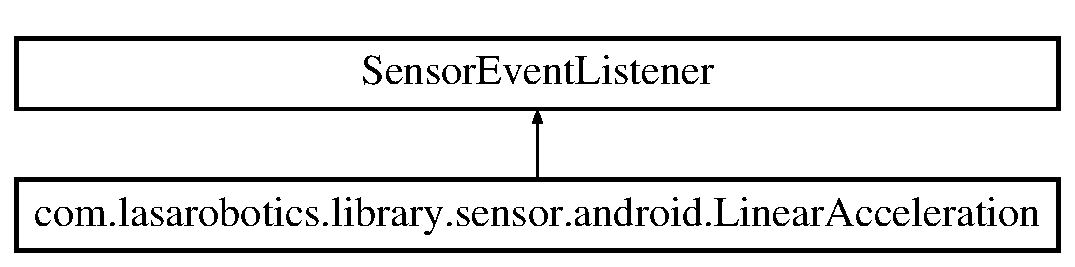
\includegraphics[height=2.000000cm]{classcom_1_1lasarobotics_1_1library_1_1sensor_1_1android_1_1_linear_acceleration}
\end{center}
\end{figure}
\subsection*{Public Member Functions}
\begin{DoxyCompactItemize}
\item 
\hypertarget{classcom_1_1lasarobotics_1_1library_1_1sensor_1_1android_1_1_linear_acceleration_aa5b483fdaba04afd6eea346b788dabfb}{}void {\bfseries on\+Accuracy\+Changed} (Sensor sensor, int i)\label{classcom_1_1lasarobotics_1_1library_1_1sensor_1_1android_1_1_linear_acceleration_aa5b483fdaba04afd6eea346b788dabfb}

\item 
\hypertarget{classcom_1_1lasarobotics_1_1library_1_1sensor_1_1android_1_1_linear_acceleration_a6b5631b1f2884acd718af8385adebff7}{}void {\bfseries on\+Sensor\+Changed} (Sensor\+Event event)\label{classcom_1_1lasarobotics_1_1library_1_1sensor_1_1android_1_1_linear_acceleration_a6b5631b1f2884acd718af8385adebff7}

\item 
\hypertarget{classcom_1_1lasarobotics_1_1library_1_1sensor_1_1android_1_1_linear_acceleration_a19ddb08608afdd29e77360e9a6cd13e5}{}\hyperlink{classcom_1_1lasarobotics_1_1library_1_1util_1_1_vector3}{Vector3}$<$ Float $>$ {\bfseries get\+Acceleration} ()\label{classcom_1_1lasarobotics_1_1library_1_1sensor_1_1android_1_1_linear_acceleration_a19ddb08608afdd29e77360e9a6cd13e5}

\end{DoxyCompactItemize}


\subsection{Detailed Description}
Gets the forces placed upon the object in the x, y, and z directions excluding gravity in m/s$^\wedge$2 

The documentation for this class was generated from the following file\+:\begin{DoxyCompactItemize}
\item 
ftc-\/library/src/main/java/com/lasarobotics/library/sensor/android/Linear\+Acceleration.\+java\end{DoxyCompactItemize}

\hypertarget{classcom_1_1lasarobotics_1_1library_1_1util_1_1_lookup_table}{}\section{com.\+lasarobotics.\+library.\+util.\+Lookup\+Table$<$ T $>$ Class Template Reference}
\label{classcom_1_1lasarobotics_1_1library_1_1util_1_1_lookup_table}\index{com.\+lasarobotics.\+library.\+util.\+Lookup\+Table$<$ T $>$@{com.\+lasarobotics.\+library.\+util.\+Lookup\+Table$<$ T $>$}}
\subsection*{Public Member Functions}
\begin{DoxyCompactItemize}
\item 
\hyperlink{classcom_1_1lasarobotics_1_1library_1_1util_1_1_lookup_table_acc7f40d76adc0c9ef5af49cf44af7929}{Lookup\+Table} ()
\item 
\hyperlink{classcom_1_1lasarobotics_1_1library_1_1util_1_1_lookup_table_af95827a058b619d3f98324fae15cb24c}{Lookup\+Table} (Hashtable$<$ String, T $>$ other)
\item 
\hyperlink{classcom_1_1lasarobotics_1_1library_1_1util_1_1_lookup_table_a01db510c04a8a9c299e5958285f4cac0}{Lookup\+Table} (\hyperlink{classcom_1_1lasarobotics_1_1library_1_1util_1_1_lookup_table}{Lookup\+Table}$<$ T $>$ other)
\item 
void \hyperlink{classcom_1_1lasarobotics_1_1library_1_1util_1_1_lookup_table_a1ace1666dc3340fe969e0161031094db}{set\+Value} (String id, T value)
\item 
T \hyperlink{classcom_1_1lasarobotics_1_1library_1_1util_1_1_lookup_table_a468df4f143f2103485ddda43ecdc98fc}{get\+Value} (String id)
\item 
void \hyperlink{classcom_1_1lasarobotics_1_1library_1_1util_1_1_lookup_table_aa9a47eda22918f48045fd0e9ef49eedb}{delete\+Value} (String id)
\item 
int \hyperlink{classcom_1_1lasarobotics_1_1library_1_1util_1_1_lookup_table_a9be202b6492a8acb988d23d829de76cb}{count} ()
\end{DoxyCompactItemize}
\subsection*{Protected Member Functions}
\begin{DoxyCompactItemize}
\item 
Hashtable$<$ String, T $>$ \hyperlink{classcom_1_1lasarobotics_1_1library_1_1util_1_1_lookup_table_a6355cca75e147643b09a7a3c9898eca7}{get\+Table} ()
\end{DoxyCompactItemize}


\subsection{Detailed Description}
Implements a variable L\+U\+T. 

\subsection{Constructor \& Destructor Documentation}
\hypertarget{classcom_1_1lasarobotics_1_1library_1_1util_1_1_lookup_table_acc7f40d76adc0c9ef5af49cf44af7929}{}\index{com\+::lasarobotics\+::library\+::util\+::\+Lookup\+Table@{com\+::lasarobotics\+::library\+::util\+::\+Lookup\+Table}!Lookup\+Table@{Lookup\+Table}}
\index{Lookup\+Table@{Lookup\+Table}!com\+::lasarobotics\+::library\+::util\+::\+Lookup\+Table@{com\+::lasarobotics\+::library\+::util\+::\+Lookup\+Table}}
\subsubsection[{Lookup\+Table()}]{\setlength{\rightskip}{0pt plus 5cm}{\bf com.\+lasarobotics.\+library.\+util.\+Lookup\+Table}$<$ T $>$.{\bf Lookup\+Table} (
\begin{DoxyParamCaption}
{}
\end{DoxyParamCaption}
)}\label{classcom_1_1lasarobotics_1_1library_1_1util_1_1_lookup_table_acc7f40d76adc0c9ef5af49cf44af7929}
Instantiate a lookup table for variables. \hypertarget{classcom_1_1lasarobotics_1_1library_1_1util_1_1_lookup_table_af95827a058b619d3f98324fae15cb24c}{}\index{com\+::lasarobotics\+::library\+::util\+::\+Lookup\+Table@{com\+::lasarobotics\+::library\+::util\+::\+Lookup\+Table}!Lookup\+Table@{Lookup\+Table}}
\index{Lookup\+Table@{Lookup\+Table}!com\+::lasarobotics\+::library\+::util\+::\+Lookup\+Table@{com\+::lasarobotics\+::library\+::util\+::\+Lookup\+Table}}
\subsubsection[{Lookup\+Table(\+Hashtable$<$ String, T $>$ other)}]{\setlength{\rightskip}{0pt plus 5cm}{\bf com.\+lasarobotics.\+library.\+util.\+Lookup\+Table}$<$ T $>$.{\bf Lookup\+Table} (
\begin{DoxyParamCaption}
\item[{Hashtable$<$ String, T $>$}]{other}
\end{DoxyParamCaption}
)}\label{classcom_1_1lasarobotics_1_1library_1_1util_1_1_lookup_table_af95827a058b619d3f98324fae15cb24c}
Create a clone from another Hashtable. 
\begin{DoxyParams}{Parameters}
{\em other} & Another Hashtable. \\
\hline
\end{DoxyParams}
\hypertarget{classcom_1_1lasarobotics_1_1library_1_1util_1_1_lookup_table_a01db510c04a8a9c299e5958285f4cac0}{}\index{com\+::lasarobotics\+::library\+::util\+::\+Lookup\+Table@{com\+::lasarobotics\+::library\+::util\+::\+Lookup\+Table}!Lookup\+Table@{Lookup\+Table}}
\index{Lookup\+Table@{Lookup\+Table}!com\+::lasarobotics\+::library\+::util\+::\+Lookup\+Table@{com\+::lasarobotics\+::library\+::util\+::\+Lookup\+Table}}
\subsubsection[{Lookup\+Table(\+Lookup\+Table$<$ T $>$ other)}]{\setlength{\rightskip}{0pt plus 5cm}{\bf com.\+lasarobotics.\+library.\+util.\+Lookup\+Table}$<$ T $>$.{\bf Lookup\+Table} (
\begin{DoxyParamCaption}
\item[{{\bf Lookup\+Table}$<$ T $>$}]{other}
\end{DoxyParamCaption}
)}\label{classcom_1_1lasarobotics_1_1library_1_1util_1_1_lookup_table_a01db510c04a8a9c299e5958285f4cac0}
Create a clone based on another \hyperlink{classcom_1_1lasarobotics_1_1library_1_1util_1_1_lookup_table}{Lookup\+Table}. 
\begin{DoxyParams}{Parameters}
{\em other} & Another \hyperlink{classcom_1_1lasarobotics_1_1library_1_1util_1_1_lookup_table}{Lookup\+Table} of the same type. \\
\hline
\end{DoxyParams}


\subsection{Member Function Documentation}
\hypertarget{classcom_1_1lasarobotics_1_1library_1_1util_1_1_lookup_table_a9be202b6492a8acb988d23d829de76cb}{}\index{com\+::lasarobotics\+::library\+::util\+::\+Lookup\+Table@{com\+::lasarobotics\+::library\+::util\+::\+Lookup\+Table}!count@{count}}
\index{count@{count}!com\+::lasarobotics\+::library\+::util\+::\+Lookup\+Table@{com\+::lasarobotics\+::library\+::util\+::\+Lookup\+Table}}
\subsubsection[{count()}]{\setlength{\rightskip}{0pt plus 5cm}int {\bf com.\+lasarobotics.\+library.\+util.\+Lookup\+Table}$<$ T $>$.count (
\begin{DoxyParamCaption}
{}
\end{DoxyParamCaption}
)}\label{classcom_1_1lasarobotics_1_1library_1_1util_1_1_lookup_table_a9be202b6492a8acb988d23d829de76cb}
The count of items in the table. \begin{DoxyReturn}{Returns}
The count of items in the table. 
\end{DoxyReturn}
\hypertarget{classcom_1_1lasarobotics_1_1library_1_1util_1_1_lookup_table_aa9a47eda22918f48045fd0e9ef49eedb}{}\index{com\+::lasarobotics\+::library\+::util\+::\+Lookup\+Table@{com\+::lasarobotics\+::library\+::util\+::\+Lookup\+Table}!delete\+Value@{delete\+Value}}
\index{delete\+Value@{delete\+Value}!com\+::lasarobotics\+::library\+::util\+::\+Lookup\+Table@{com\+::lasarobotics\+::library\+::util\+::\+Lookup\+Table}}
\subsubsection[{delete\+Value(\+String id)}]{\setlength{\rightskip}{0pt plus 5cm}void {\bf com.\+lasarobotics.\+library.\+util.\+Lookup\+Table}$<$ T $>$.delete\+Value (
\begin{DoxyParamCaption}
\item[{String}]{id}
\end{DoxyParamCaption}
)}\label{classcom_1_1lasarobotics_1_1library_1_1util_1_1_lookup_table_aa9a47eda22918f48045fd0e9ef49eedb}
Remove a value from the table at a specific I\+D. 
\begin{DoxyParams}{Parameters}
{\em id} & The I\+D of an item in the table. \\
\hline
\end{DoxyParams}
\hypertarget{classcom_1_1lasarobotics_1_1library_1_1util_1_1_lookup_table_a6355cca75e147643b09a7a3c9898eca7}{}\index{com\+::lasarobotics\+::library\+::util\+::\+Lookup\+Table@{com\+::lasarobotics\+::library\+::util\+::\+Lookup\+Table}!get\+Table@{get\+Table}}
\index{get\+Table@{get\+Table}!com\+::lasarobotics\+::library\+::util\+::\+Lookup\+Table@{com\+::lasarobotics\+::library\+::util\+::\+Lookup\+Table}}
\subsubsection[{get\+Table()}]{\setlength{\rightskip}{0pt plus 5cm}Hashtable$<$String, T$>$ {\bf com.\+lasarobotics.\+library.\+util.\+Lookup\+Table}$<$ T $>$.get\+Table (
\begin{DoxyParamCaption}
{}
\end{DoxyParamCaption}
)\hspace{0.3cm}{\ttfamily [protected]}}\label{classcom_1_1lasarobotics_1_1library_1_1util_1_1_lookup_table_a6355cca75e147643b09a7a3c9898eca7}
Gets the underlying Hashtable instance. \begin{DoxyReturn}{Returns}
The underlying Hashtable. 
\end{DoxyReturn}
\hypertarget{classcom_1_1lasarobotics_1_1library_1_1util_1_1_lookup_table_a468df4f143f2103485ddda43ecdc98fc}{}\index{com\+::lasarobotics\+::library\+::util\+::\+Lookup\+Table@{com\+::lasarobotics\+::library\+::util\+::\+Lookup\+Table}!get\+Value@{get\+Value}}
\index{get\+Value@{get\+Value}!com\+::lasarobotics\+::library\+::util\+::\+Lookup\+Table@{com\+::lasarobotics\+::library\+::util\+::\+Lookup\+Table}}
\subsubsection[{get\+Value(\+String id)}]{\setlength{\rightskip}{0pt plus 5cm}T {\bf com.\+lasarobotics.\+library.\+util.\+Lookup\+Table}$<$ T $>$.get\+Value (
\begin{DoxyParamCaption}
\item[{String}]{id}
\end{DoxyParamCaption}
)}\label{classcom_1_1lasarobotics_1_1library_1_1util_1_1_lookup_table_a468df4f143f2103485ddda43ecdc98fc}
Get the value of an id in the L\+U\+T. 
\begin{DoxyParams}{Parameters}
{\em id} & The I\+D of the item to retrieve. \\
\hline
\end{DoxyParams}
\begin{DoxyReturn}{Returns}
The value of the item at the id. 
\end{DoxyReturn}
\hypertarget{classcom_1_1lasarobotics_1_1library_1_1util_1_1_lookup_table_a1ace1666dc3340fe969e0161031094db}{}\index{com\+::lasarobotics\+::library\+::util\+::\+Lookup\+Table@{com\+::lasarobotics\+::library\+::util\+::\+Lookup\+Table}!set\+Value@{set\+Value}}
\index{set\+Value@{set\+Value}!com\+::lasarobotics\+::library\+::util\+::\+Lookup\+Table@{com\+::lasarobotics\+::library\+::util\+::\+Lookup\+Table}}
\subsubsection[{set\+Value(\+String id, T value)}]{\setlength{\rightskip}{0pt plus 5cm}void {\bf com.\+lasarobotics.\+library.\+util.\+Lookup\+Table}$<$ T $>$.set\+Value (
\begin{DoxyParamCaption}
\item[{String}]{id, }
\item[{T}]{value}
\end{DoxyParamCaption}
)}\label{classcom_1_1lasarobotics_1_1library_1_1util_1_1_lookup_table_a1ace1666dc3340fe969e0161031094db}
Set the value of an item in the table, or create if new. 
\begin{DoxyParams}{Parameters}
{\em id} & The I\+D of the item in the L\+U\+T. \\
\hline
{\em value} & The value to set the id to. \\
\hline
\end{DoxyParams}


The documentation for this class was generated from the following file\+:\begin{DoxyCompactItemize}
\item 
ftc-\/library/src/main/java/com/lasarobotics/library/util/Lookup\+Table.\+java\end{DoxyCompactItemize}

\hypertarget{classcom_1_1lasarobotics_1_1library_1_1util_1_1_math_util}{}\section{com.\+lasarobotics.\+library.\+util.\+Math\+Util Class Reference}
\label{classcom_1_1lasarobotics_1_1library_1_1util_1_1_math_util}\index{com.\+lasarobotics.\+library.\+util.\+Math\+Util@{com.\+lasarobotics.\+library.\+util.\+Math\+Util}}
\subsection*{Static Public Member Functions}
\begin{DoxyCompactItemize}
\item 
static double \hyperlink{classcom_1_1lasarobotics_1_1library_1_1util_1_1_math_util_a4669403ad7a53281e54642b19c854969}{deadband} (double deadband, double value)
\item 
static Boolean \hyperlink{classcom_1_1lasarobotics_1_1library_1_1util_1_1_math_util_a237a2132ae1166ad3860162c43772c8d}{equal} (double a, double b)
\item 
static Boolean \hyperlink{classcom_1_1lasarobotics_1_1library_1_1util_1_1_math_util_a4a0d5166631ce63f29831cddcc93606c}{equal} (double a, double b, double distance)
\item 
static double \hyperlink{classcom_1_1lasarobotics_1_1library_1_1util_1_1_math_util_ad4f61bfb6db04221bfa2ae604294212b}{filter} (double value, double lastvalue, double fail)
\item 
static double \hyperlink{classcom_1_1lasarobotics_1_1library_1_1util_1_1_math_util_ad104d4e18dfb7085f1df06cc06e1181d}{coerce} (double min, double max, double value)
\item 
static boolean \hyperlink{classcom_1_1lasarobotics_1_1library_1_1util_1_1_math_util_abf940081e2bc48457b82db587b9e19cd}{in\+Bounds} (double min, double max, double value)
\end{DoxyCompactItemize}


\subsection{Detailed Description}
Mathematical and Precision Utilities 

\subsection{Member Function Documentation}
\hypertarget{classcom_1_1lasarobotics_1_1library_1_1util_1_1_math_util_ad104d4e18dfb7085f1df06cc06e1181d}{}\index{com\+::lasarobotics\+::library\+::util\+::\+Math\+Util@{com\+::lasarobotics\+::library\+::util\+::\+Math\+Util}!coerce@{coerce}}
\index{coerce@{coerce}!com\+::lasarobotics\+::library\+::util\+::\+Math\+Util@{com\+::lasarobotics\+::library\+::util\+::\+Math\+Util}}
\subsubsection[{coerce(double min, double max, double value)}]{\setlength{\rightskip}{0pt plus 5cm}static double com.\+lasarobotics.\+library.\+util.\+Math\+Util.\+coerce (
\begin{DoxyParamCaption}
\item[{double}]{min, }
\item[{double}]{max, }
\item[{double}]{value}
\end{DoxyParamCaption}
)\hspace{0.3cm}{\ttfamily [static]}}\label{classcom_1_1lasarobotics_1_1library_1_1util_1_1_math_util_ad104d4e18dfb7085f1df06cc06e1181d}
Forces a numerical value to be between a min and a max


\begin{DoxyParams}{Parameters}
{\em min} & If less than min, returns min \\
\hline
{\em max} & If greater than max, returns max \\
\hline
{\em value} & Value to test \\
\hline
\end{DoxyParams}
\begin{DoxyReturn}{Returns}
Coerced value 
\end{DoxyReturn}
\hypertarget{classcom_1_1lasarobotics_1_1library_1_1util_1_1_math_util_a4669403ad7a53281e54642b19c854969}{}\index{com\+::lasarobotics\+::library\+::util\+::\+Math\+Util@{com\+::lasarobotics\+::library\+::util\+::\+Math\+Util}!deadband@{deadband}}
\index{deadband@{deadband}!com\+::lasarobotics\+::library\+::util\+::\+Math\+Util@{com\+::lasarobotics\+::library\+::util\+::\+Math\+Util}}
\subsubsection[{deadband(double deadband, double value)}]{\setlength{\rightskip}{0pt plus 5cm}static double com.\+lasarobotics.\+library.\+util.\+Math\+Util.\+deadband (
\begin{DoxyParamCaption}
\item[{double}]{deadband, }
\item[{double}]{value}
\end{DoxyParamCaption}
)\hspace{0.3cm}{\ttfamily [static]}}\label{classcom_1_1lasarobotics_1_1library_1_1util_1_1_math_util_a4669403ad7a53281e54642b19c854969}
Gives a \char`\"{}deadzone\char`\"{} where any value less than this would return zero.


\begin{DoxyParams}{Parameters}
{\em deadband} & Maximum value that returns zero \\
\hline
{\em value} & Value to test \\
\hline
\end{DoxyParams}
\begin{DoxyReturn}{Returns}
Deadbanded value 
\end{DoxyReturn}
\hypertarget{classcom_1_1lasarobotics_1_1library_1_1util_1_1_math_util_a237a2132ae1166ad3860162c43772c8d}{}\index{com\+::lasarobotics\+::library\+::util\+::\+Math\+Util@{com\+::lasarobotics\+::library\+::util\+::\+Math\+Util}!equal@{equal}}
\index{equal@{equal}!com\+::lasarobotics\+::library\+::util\+::\+Math\+Util@{com\+::lasarobotics\+::library\+::util\+::\+Math\+Util}}
\subsubsection[{equal(double a, double b)}]{\setlength{\rightskip}{0pt plus 5cm}static Boolean com.\+lasarobotics.\+library.\+util.\+Math\+Util.\+equal (
\begin{DoxyParamCaption}
\item[{double}]{a, }
\item[{double}]{b}
\end{DoxyParamCaption}
)\hspace{0.3cm}{\ttfamily [static]}}\label{classcom_1_1lasarobotics_1_1library_1_1util_1_1_math_util_a237a2132ae1166ad3860162c43772c8d}
Returns if two double values are equal to within epsilon. 
\begin{DoxyParams}{Parameters}
{\em a} & First value \\
\hline
{\em b} & Second value \\
\hline
\end{DoxyParams}
\begin{DoxyReturn}{Returns}
True if the values are equal, false otherwise 
\end{DoxyReturn}
\hypertarget{classcom_1_1lasarobotics_1_1library_1_1util_1_1_math_util_a4a0d5166631ce63f29831cddcc93606c}{}\index{com\+::lasarobotics\+::library\+::util\+::\+Math\+Util@{com\+::lasarobotics\+::library\+::util\+::\+Math\+Util}!equal@{equal}}
\index{equal@{equal}!com\+::lasarobotics\+::library\+::util\+::\+Math\+Util@{com\+::lasarobotics\+::library\+::util\+::\+Math\+Util}}
\subsubsection[{equal(double a, double b, double distance)}]{\setlength{\rightskip}{0pt plus 5cm}static Boolean com.\+lasarobotics.\+library.\+util.\+Math\+Util.\+equal (
\begin{DoxyParamCaption}
\item[{double}]{a, }
\item[{double}]{b, }
\item[{double}]{distance}
\end{DoxyParamCaption}
)\hspace{0.3cm}{\ttfamily [static]}}\label{classcom_1_1lasarobotics_1_1library_1_1util_1_1_math_util_a4a0d5166631ce63f29831cddcc93606c}
Returns if two double values are equal to within a distance. 
\begin{DoxyParams}{Parameters}
{\em a} & First value \\
\hline
{\em b} & Second value \\
\hline
{\em distance} & Maximum distance between a and b \\
\hline
\end{DoxyParams}
\begin{DoxyReturn}{Returns}
True if the values are equal ot within distance, false otherwise 
\end{DoxyReturn}
\hypertarget{classcom_1_1lasarobotics_1_1library_1_1util_1_1_math_util_ad4f61bfb6db04221bfa2ae604294212b}{}\index{com\+::lasarobotics\+::library\+::util\+::\+Math\+Util@{com\+::lasarobotics\+::library\+::util\+::\+Math\+Util}!filter@{filter}}
\index{filter@{filter}!com\+::lasarobotics\+::library\+::util\+::\+Math\+Util@{com\+::lasarobotics\+::library\+::util\+::\+Math\+Util}}
\subsubsection[{filter(double value, double lastvalue, double fail)}]{\setlength{\rightskip}{0pt plus 5cm}static double com.\+lasarobotics.\+library.\+util.\+Math\+Util.\+filter (
\begin{DoxyParamCaption}
\item[{double}]{value, }
\item[{double}]{lastvalue, }
\item[{double}]{fail}
\end{DoxyParamCaption}
)\hspace{0.3cm}{\ttfamily [static]}}\label{classcom_1_1lasarobotics_1_1library_1_1util_1_1_math_util_ad4f61bfb6db04221bfa2ae604294212b}
Ignores values equal to the fail value (normally zero). 
\begin{DoxyParams}{Parameters}
{\em value} & Current value \\
\hline
{\em lastvalue} & Previous value \\
\hline
{\em fail} & Filter this value, normally zero \\
\hline
\end{DoxyParams}
\begin{DoxyReturn}{Returns}
Filtered value 
\end{DoxyReturn}
\hypertarget{classcom_1_1lasarobotics_1_1library_1_1util_1_1_math_util_abf940081e2bc48457b82db587b9e19cd}{}\index{com\+::lasarobotics\+::library\+::util\+::\+Math\+Util@{com\+::lasarobotics\+::library\+::util\+::\+Math\+Util}!in\+Bounds@{in\+Bounds}}
\index{in\+Bounds@{in\+Bounds}!com\+::lasarobotics\+::library\+::util\+::\+Math\+Util@{com\+::lasarobotics\+::library\+::util\+::\+Math\+Util}}
\subsubsection[{in\+Bounds(double min, double max, double value)}]{\setlength{\rightskip}{0pt plus 5cm}static boolean com.\+lasarobotics.\+library.\+util.\+Math\+Util.\+in\+Bounds (
\begin{DoxyParamCaption}
\item[{double}]{min, }
\item[{double}]{max, }
\item[{double}]{value}
\end{DoxyParamCaption}
)\hspace{0.3cm}{\ttfamily [static]}}\label{classcom_1_1lasarobotics_1_1library_1_1util_1_1_math_util_abf940081e2bc48457b82db587b9e19cd}
Tests if a number is between the bounds, inclusive.


\begin{DoxyParams}{Parameters}
{\em min} & If less than min, returns false \\
\hline
{\em max} & If greater than max, returns false \\
\hline
{\em value} & Value to test \\
\hline
\end{DoxyParams}
\begin{DoxyReturn}{Returns}
Returns true if value is between (inclusive) min and max, false otherwise. 
\end{DoxyReturn}


The documentation for this class was generated from the following file\+:\begin{DoxyCompactItemize}
\item 
ftc-\/library/src/main/java/com/lasarobotics/library/util/Math\+Util.\+java\end{DoxyCompactItemize}

\hypertarget{classcom_1_1lasarobotics_1_1library_1_1drive_1_1_mecanum}{}\section{com.\+lasarobotics.\+library.\+drive.\+Mecanum Class Reference}
\label{classcom_1_1lasarobotics_1_1library_1_1drive_1_1_mecanum}\index{com.\+lasarobotics.\+library.\+drive.\+Mecanum@{com.\+lasarobotics.\+library.\+drive.\+Mecanum}}
\subsection*{Static Public Member Functions}
\begin{DoxyCompactItemize}
\item 
static void \hyperlink{classcom_1_1lasarobotics_1_1library_1_1drive_1_1_mecanum_a8ab2eabd44ba148744ca3480484e731b}{Arcade} (double y, double x, double c, Dc\+Motor left\+Front, Dc\+Motor right\+Front, Dc\+Motor left\+Back, Dc\+Motor right\+Back)
\item 
static void \hyperlink{classcom_1_1lasarobotics_1_1library_1_1drive_1_1_mecanum_a2a6039a767b1a6aa175f5c28ef8f33bd}{Arcade\+\_\+\+Field\+Oriented} (double y, double x, double c, double gyroheading, Dc\+Motor left\+Front, Dc\+Motor right\+Front, Dc\+Motor left\+Back, Dc\+Motor right\+Back)
\end{DoxyCompactItemize}


\subsection{Detailed Description}
Methods for the \hyperlink{classcom_1_1lasarobotics_1_1library_1_1drive_1_1_mecanum}{Mecanum} multi-\/directional drive train 

\subsection{Member Function Documentation}
\hypertarget{classcom_1_1lasarobotics_1_1library_1_1drive_1_1_mecanum_a8ab2eabd44ba148744ca3480484e731b}{}\index{com\+::lasarobotics\+::library\+::drive\+::\+Mecanum@{com\+::lasarobotics\+::library\+::drive\+::\+Mecanum}!Arcade@{Arcade}}
\index{Arcade@{Arcade}!com\+::lasarobotics\+::library\+::drive\+::\+Mecanum@{com\+::lasarobotics\+::library\+::drive\+::\+Mecanum}}
\subsubsection[{Arcade(double y, double x, double c, Dc\+Motor left\+Front, Dc\+Motor right\+Front, Dc\+Motor left\+Back, Dc\+Motor right\+Back)}]{\setlength{\rightskip}{0pt plus 5cm}static void com.\+lasarobotics.\+library.\+drive.\+Mecanum.\+Arcade (
\begin{DoxyParamCaption}
\item[{double}]{y, }
\item[{double}]{x, }
\item[{double}]{c, }
\item[{Dc\+Motor}]{left\+Front, }
\item[{Dc\+Motor}]{right\+Front, }
\item[{Dc\+Motor}]{left\+Back, }
\item[{Dc\+Motor}]{right\+Back}
\end{DoxyParamCaption}
)\hspace{0.3cm}{\ttfamily [static]}}\label{classcom_1_1lasarobotics_1_1library_1_1drive_1_1_mecanum_a8ab2eabd44ba148744ca3480484e731b}
Implements the Arcade drive train with three axis and four motors. 
\begin{DoxyParams}{Parameters}
{\em y} & The y-\/axis of the controller, forward/rev \\
\hline
{\em x} & The x-\/axis of the controller, strafe \\
\hline
{\em c} & The spin axis of the controller \\
\hline
{\em left\+Front} & The motor on the front left \\
\hline
{\em right\+Front} & The motor on the front right \\
\hline
{\em left\+Back} & The motor on the back left \\
\hline
{\em right\+Back} & The motor on the back right \\
\hline
\end{DoxyParams}
\hypertarget{classcom_1_1lasarobotics_1_1library_1_1drive_1_1_mecanum_a2a6039a767b1a6aa175f5c28ef8f33bd}{}\index{com\+::lasarobotics\+::library\+::drive\+::\+Mecanum@{com\+::lasarobotics\+::library\+::drive\+::\+Mecanum}!Arcade\+\_\+\+Field\+Oriented@{Arcade\+\_\+\+Field\+Oriented}}
\index{Arcade\+\_\+\+Field\+Oriented@{Arcade\+\_\+\+Field\+Oriented}!com\+::lasarobotics\+::library\+::drive\+::\+Mecanum@{com\+::lasarobotics\+::library\+::drive\+::\+Mecanum}}
\subsubsection[{Arcade\+\_\+\+Field\+Oriented(double y, double x, double c, double gyroheading, Dc\+Motor left\+Front, Dc\+Motor right\+Front, Dc\+Motor left\+Back, Dc\+Motor right\+Back)}]{\setlength{\rightskip}{0pt plus 5cm}static void com.\+lasarobotics.\+library.\+drive.\+Mecanum.\+Arcade\+\_\+\+Field\+Oriented (
\begin{DoxyParamCaption}
\item[{double}]{y, }
\item[{double}]{x, }
\item[{double}]{c, }
\item[{double}]{gyroheading, }
\item[{Dc\+Motor}]{left\+Front, }
\item[{Dc\+Motor}]{right\+Front, }
\item[{Dc\+Motor}]{left\+Back, }
\item[{Dc\+Motor}]{right\+Back}
\end{DoxyParamCaption}
)\hspace{0.3cm}{\ttfamily [static]}}\label{classcom_1_1lasarobotics_1_1library_1_1drive_1_1_mecanum_a2a6039a767b1a6aa175f5c28ef8f33bd}
Implements the Arcade drive train with field orientation based on Gyro input 
\begin{DoxyParams}{Parameters}
{\em y} & The y-\/axis of the controller, forward/rev \\
\hline
{\em x} & The x-\/axis of the controller, strafe \\
\hline
{\em c} & The spin axis of the controller \\
\hline
{\em gyroheading} & The current normalized gyro heading (between 0 and 360) \\
\hline
{\em left\+Front} & The motor on the front left \\
\hline
{\em right\+Front} & The motor on the front right \\
\hline
{\em left\+Back} & The motor on the back left \\
\hline
{\em right\+Back} & The motor on the back right \\
\hline
\end{DoxyParams}


The documentation for this class was generated from the following file\+:\begin{DoxyCompactItemize}
\item 
ftc-\/library/src/main/java/com/lasarobotics/library/drive/Mecanum.\+java\end{DoxyCompactItemize}

\hypertarget{classcom_1_1lasarobotics_1_1library_1_1monkeyc_1_1_monkey_c}{}\section{com.\+lasarobotics.\+library.\+monkeyc.\+Monkey\+C Class Reference}
\label{classcom_1_1lasarobotics_1_1library_1_1monkeyc_1_1_monkey_c}\index{com.\+lasarobotics.\+library.\+monkeyc.\+Monkey\+C@{com.\+lasarobotics.\+library.\+monkeyc.\+Monkey\+C}}
\subsection*{Public Member Functions}
\begin{DoxyCompactItemize}
\item 
\hypertarget{classcom_1_1lasarobotics_1_1library_1_1monkeyc_1_1_monkey_c_a2bc7a1f53adfbfe2cdbb19c456c7b226}{}void {\bfseries add} (\hyperlink{classcom_1_1lasarobotics_1_1library_1_1controller_1_1_controller}{Controller} c1, \hyperlink{classcom_1_1lasarobotics_1_1library_1_1controller_1_1_controller}{Controller} c2)\label{classcom_1_1lasarobotics_1_1library_1_1monkeyc_1_1_monkey_c_a2bc7a1f53adfbfe2cdbb19c456c7b226}

\item 
\hypertarget{classcom_1_1lasarobotics_1_1library_1_1monkeyc_1_1_monkey_c_afceca05780b824278b087f622272e687}{}void {\bfseries add} (Gamepad instruction, Gamepad instruction2)\label{classcom_1_1lasarobotics_1_1library_1_1monkeyc_1_1_monkey_c_afceca05780b824278b087f622272e687}

\item 
\hypertarget{classcom_1_1lasarobotics_1_1library_1_1monkeyc_1_1_monkey_c_a7ac34bb6c6f82809cb68883a127f597e}{}void {\bfseries clear} ()\label{classcom_1_1lasarobotics_1_1library_1_1monkeyc_1_1_monkey_c_a7ac34bb6c6f82809cb68883a127f597e}

\item 
\hypertarget{classcom_1_1lasarobotics_1_1library_1_1monkeyc_1_1_monkey_c_a4c81116b676a38f6f89d486f2828575f}{}void {\bfseries write} (String filename, Context context)\label{classcom_1_1lasarobotics_1_1library_1_1monkeyc_1_1_monkey_c_a4c81116b676a38f6f89d486f2828575f}

\item 
\hypertarget{classcom_1_1lasarobotics_1_1library_1_1monkeyc_1_1_monkey_c_ad5fbc45ad3969c57a36477434b01bb95}{}int {\bfseries size} ()\label{classcom_1_1lasarobotics_1_1library_1_1monkeyc_1_1_monkey_c_ad5fbc45ad3969c57a36477434b01bb95}

\end{DoxyCompactItemize}


\subsection{Detailed Description}
The \hyperlink{classcom_1_1lasarobotics_1_1library_1_1monkeyc_1_1_monkey_c}{Monkey\+C} (Monkey\+See) library that handles recording and storing driver controls These controls can be inserted during runtime (when the robot is moving) or can be created prior to a match. \hyperlink{classcom_1_1lasarobotics_1_1library_1_1monkeyc_1_1_monkey_do}{Monkey\+Do} can then execute these commands. 

The documentation for this class was generated from the following file\+:\begin{DoxyCompactItemize}
\item 
ftc-\/library/src/main/java/com/lasarobotics/library/monkeyc/Monkey\+C.\+java\end{DoxyCompactItemize}

\hypertarget{classcom_1_1lasarobotics_1_1library_1_1monkeyc_1_1_monkey_data}{}\section{com.\+lasarobotics.\+library.\+monkeyc.\+Monkey\+Data Class Reference}
\label{classcom_1_1lasarobotics_1_1library_1_1monkeyc_1_1_monkey_data}\index{com.\+lasarobotics.\+library.\+monkeyc.\+Monkey\+Data@{com.\+lasarobotics.\+library.\+monkeyc.\+Monkey\+Data}}
\subsection*{Public Member Functions}
\begin{DoxyCompactItemize}
\item 
\hypertarget{classcom_1_1lasarobotics_1_1library_1_1monkeyc_1_1_monkey_data_a2fddb34ead2cec3619adeef4988bfb69}{}\hyperlink{classcom_1_1lasarobotics_1_1library_1_1controller_1_1_controller}{Controller} {\bfseries update\+Controller\+One} (\hyperlink{classcom_1_1lasarobotics_1_1library_1_1controller_1_1_controller}{Controller} previous)\label{classcom_1_1lasarobotics_1_1library_1_1monkeyc_1_1_monkey_data_a2fddb34ead2cec3619adeef4988bfb69}

\item 
\hypertarget{classcom_1_1lasarobotics_1_1library_1_1monkeyc_1_1_monkey_data_a3743b8283c0721a212f48c2d3b011e3f}{}\hyperlink{classcom_1_1lasarobotics_1_1library_1_1controller_1_1_controller}{Controller} {\bfseries update\+Controller\+Two} (\hyperlink{classcom_1_1lasarobotics_1_1library_1_1controller_1_1_controller}{Controller} previous)\label{classcom_1_1lasarobotics_1_1library_1_1monkeyc_1_1_monkey_data_a3743b8283c0721a212f48c2d3b011e3f}

\item 
\hypertarget{classcom_1_1lasarobotics_1_1library_1_1monkeyc_1_1_monkey_data_a3552a7d169f51d3e24921a2372ae17ce}{}boolean {\bfseries has\+Update} ()\label{classcom_1_1lasarobotics_1_1library_1_1monkeyc_1_1_monkey_data_a3552a7d169f51d3e24921a2372ae17ce}

\item 
\hypertarget{classcom_1_1lasarobotics_1_1library_1_1monkeyc_1_1_monkey_data_ae802fc3183552c0c4ba86f7f34744929}{}Json\+Object {\bfseries get\+Deltas\+Gamepad1} ()\label{classcom_1_1lasarobotics_1_1library_1_1monkeyc_1_1_monkey_data_ae802fc3183552c0c4ba86f7f34744929}

\item 
\hypertarget{classcom_1_1lasarobotics_1_1library_1_1monkeyc_1_1_monkey_data_a727455c2818da90dea05a74193976808}{}void {\bfseries set\+Deltas\+Gamepad1} (Json\+Object deltas\+Gamepad1)\label{classcom_1_1lasarobotics_1_1library_1_1monkeyc_1_1_monkey_data_a727455c2818da90dea05a74193976808}

\item 
\hypertarget{classcom_1_1lasarobotics_1_1library_1_1monkeyc_1_1_monkey_data_aca1aba18ede7b1a10fb8ec65bb99ba95}{}Json\+Object {\bfseries get\+Deltas\+Gamepad2} ()\label{classcom_1_1lasarobotics_1_1library_1_1monkeyc_1_1_monkey_data_aca1aba18ede7b1a10fb8ec65bb99ba95}

\item 
\hypertarget{classcom_1_1lasarobotics_1_1library_1_1monkeyc_1_1_monkey_data_afc0d5a15c6cbc2bc55d2d8f2f00418f7}{}void {\bfseries set\+Deltas\+Gamepad2} (Json\+Object deltas\+Gamepad2)\label{classcom_1_1lasarobotics_1_1library_1_1monkeyc_1_1_monkey_data_afc0d5a15c6cbc2bc55d2d8f2f00418f7}

\item 
\hypertarget{classcom_1_1lasarobotics_1_1library_1_1monkeyc_1_1_monkey_data_ab5dd5e5be346d334900459e3481d9347}{}void {\bfseries set\+Time} (long time)\label{classcom_1_1lasarobotics_1_1library_1_1monkeyc_1_1_monkey_data_ab5dd5e5be346d334900459e3481d9347}

\item 
\hypertarget{classcom_1_1lasarobotics_1_1library_1_1monkeyc_1_1_monkey_data_a5a29849d0d744c500771bd5788f2857e}{}long {\bfseries get\+Time} ()\label{classcom_1_1lasarobotics_1_1library_1_1monkeyc_1_1_monkey_data_a5a29849d0d744c500771bd5788f2857e}

\end{DoxyCompactItemize}


\subsection{Detailed Description}
Contains a single time-\/stamped patched state of one Controller 

The documentation for this class was generated from the following file\+:\begin{DoxyCompactItemize}
\item 
ftc-\/library/src/main/java/com/lasarobotics/library/monkeyc/Monkey\+Data.\+java\end{DoxyCompactItemize}

\hypertarget{classcom_1_1lasarobotics_1_1library_1_1monkeyc_1_1_monkey_do}{}\section{com.\+lasarobotics.\+library.\+monkeyc.\+Monkey\+Do Class Reference}
\label{classcom_1_1lasarobotics_1_1library_1_1monkeyc_1_1_monkey_do}\index{com.\+lasarobotics.\+library.\+monkeyc.\+Monkey\+Do@{com.\+lasarobotics.\+library.\+monkeyc.\+Monkey\+Do}}
\subsection*{Public Member Functions}
\begin{DoxyCompactItemize}
\item 
\hypertarget{classcom_1_1lasarobotics_1_1library_1_1monkeyc_1_1_monkey_do_a66c4ab0129f080ad2c9521dc4d9948bd}{}{\bfseries Monkey\+Do} (String filename, Context context)\label{classcom_1_1lasarobotics_1_1library_1_1monkeyc_1_1_monkey_do_a66c4ab0129f080ad2c9521dc4d9948bd}

\item 
\hypertarget{classcom_1_1lasarobotics_1_1library_1_1monkeyc_1_1_monkey_do_ab4fabec0eb0155486246174f5bb59fcf}{}\hyperlink{classcom_1_1lasarobotics_1_1library_1_1monkeyc_1_1_monkey_data}{Monkey\+Data} {\bfseries get\+Next\+Command} ()\label{classcom_1_1lasarobotics_1_1library_1_1monkeyc_1_1_monkey_do_ab4fabec0eb0155486246174f5bb59fcf}

\item 
\hypertarget{classcom_1_1lasarobotics_1_1library_1_1monkeyc_1_1_monkey_do_a5129f21484decf70a61ff92881b975bf}{}String {\bfseries get\+Filename} ()\label{classcom_1_1lasarobotics_1_1library_1_1monkeyc_1_1_monkey_do_a5129f21484decf70a61ff92881b975bf}

\item 
\hypertarget{classcom_1_1lasarobotics_1_1library_1_1monkeyc_1_1_monkey_do_a60cdcde0db055c683338a0a6523586fb}{}void {\bfseries set\+Filename} (String filename)\label{classcom_1_1lasarobotics_1_1library_1_1monkeyc_1_1_monkey_do_a60cdcde0db055c683338a0a6523586fb}

\item 
\hypertarget{classcom_1_1lasarobotics_1_1library_1_1monkeyc_1_1_monkey_do_aea7beeeb5cdd018aa05e49b030eb9b9b}{}void {\bfseries on\+Start} ()\label{classcom_1_1lasarobotics_1_1library_1_1monkeyc_1_1_monkey_do_aea7beeeb5cdd018aa05e49b030eb9b9b}

\end{DoxyCompactItemize}


\subsection{Detailed Description}
The \hyperlink{classcom_1_1lasarobotics_1_1library_1_1monkeyc_1_1_monkey_do}{Monkey\+Do} library handles executing commands generated by \hyperlink{classcom_1_1lasarobotics_1_1library_1_1monkeyc_1_1_monkey_c}{Monkey\+C}. 

The documentation for this class was generated from the following file\+:\begin{DoxyCompactItemize}
\item 
ftc-\/library/src/main/java/com/lasarobotics/library/monkeyc/Monkey\+Do.\+java\end{DoxyCompactItemize}

\hypertarget{classcom_1_1lasarobotics_1_1library_1_1monkeyc_1_1_monkey_util}{}\section{com.\+lasarobotics.\+library.\+monkeyc.\+Monkey\+Util Class Reference}
\label{classcom_1_1lasarobotics_1_1library_1_1monkeyc_1_1_monkey_util}\index{com.\+lasarobotics.\+library.\+monkeyc.\+Monkey\+Util@{com.\+lasarobotics.\+library.\+monkeyc.\+Monkey\+Util}}
\subsection*{Static Public Member Functions}
\begin{DoxyCompactItemize}
\item 
\hypertarget{classcom_1_1lasarobotics_1_1library_1_1monkeyc_1_1_monkey_util_ad53a6656de74281de2c0e32b0a7a04f5}{}static \hyperlink{classcom_1_1lasarobotics_1_1library_1_1monkeyc_1_1_monkey_data}{Monkey\+Data} {\bfseries create\+Deltas} (\hyperlink{classcom_1_1lasarobotics_1_1library_1_1controller_1_1_controller}{Controller} current1, \hyperlink{classcom_1_1lasarobotics_1_1library_1_1controller_1_1_controller}{Controller} previous1, \hyperlink{classcom_1_1lasarobotics_1_1library_1_1controller_1_1_controller}{Controller} current2, \hyperlink{classcom_1_1lasarobotics_1_1library_1_1controller_1_1_controller}{Controller} previous2, long time)\label{classcom_1_1lasarobotics_1_1library_1_1monkeyc_1_1_monkey_util_ad53a6656de74281de2c0e32b0a7a04f5}

\item 
\hypertarget{classcom_1_1lasarobotics_1_1library_1_1monkeyc_1_1_monkey_util_a110938b02fc52187735d141c7099b9ec}{}static void {\bfseries write\+File} (String filename, Array\+List$<$ \hyperlink{classcom_1_1lasarobotics_1_1library_1_1monkeyc_1_1_monkey_data}{Monkey\+Data} $>$ commands, Context context)\label{classcom_1_1lasarobotics_1_1library_1_1monkeyc_1_1_monkey_util_a110938b02fc52187735d141c7099b9ec}

\item 
\hypertarget{classcom_1_1lasarobotics_1_1library_1_1monkeyc_1_1_monkey_util_a957c31e9a0f2a187d1e87540b94a88d9}{}static Array\+List$<$ \hyperlink{classcom_1_1lasarobotics_1_1library_1_1monkeyc_1_1_monkey_data}{Monkey\+Data} $>$ {\bfseries read\+File} (String filename, Context context)\label{classcom_1_1lasarobotics_1_1library_1_1monkeyc_1_1_monkey_util_a957c31e9a0f2a187d1e87540b94a88d9}

\end{DoxyCompactItemize}
\subsection*{Static Public Attributes}
\begin{DoxyCompactItemize}
\item 
\hypertarget{classcom_1_1lasarobotics_1_1library_1_1monkeyc_1_1_monkey_util_a1da99dbc3d38e23e17ac51a39ea1a18b}{}static final String {\bfseries F\+I\+L\+E\+\_\+\+D\+I\+R} = Environment.\+get\+External\+Storage\+Directory() + \char`\"{}/Monkey\+C/\char`\"{}\label{classcom_1_1lasarobotics_1_1library_1_1monkeyc_1_1_monkey_util_a1da99dbc3d38e23e17ac51a39ea1a18b}

\end{DoxyCompactItemize}


\subsection{Detailed Description}
\hyperlink{classcom_1_1lasarobotics_1_1library_1_1monkeyc_1_1_monkey_util}{Monkey\+Util} handles reading and writing text files with instructions created by \hyperlink{classcom_1_1lasarobotics_1_1library_1_1monkeyc_1_1_monkey_c}{Monkey\+C} 

The documentation for this class was generated from the following file\+:\begin{DoxyCompactItemize}
\item 
ftc-\/library/src/main/java/com/lasarobotics/library/monkeyc/Monkey\+Util.\+java\end{DoxyCompactItemize}

\hypertarget{classcom_1_1lasarobotics_1_1library_1_1doodle_1_1actions_1_1sensors_1_1_motor_encoder_reset}{}\section{com.\+lasarobotics.\+library.\+doodle.\+actions.\+sensors.\+Motor\+Encoder\+Reset Class Reference}
\label{classcom_1_1lasarobotics_1_1library_1_1doodle_1_1actions_1_1sensors_1_1_motor_encoder_reset}\index{com.\+lasarobotics.\+library.\+doodle.\+actions.\+sensors.\+Motor\+Encoder\+Reset@{com.\+lasarobotics.\+library.\+doodle.\+actions.\+sensors.\+Motor\+Encoder\+Reset}}


\subsection{Detailed Description}
Reset a motor encoder 

The documentation for this class was generated from the following file\+:\begin{DoxyCompactItemize}
\item 
ftc-\/library/src/main/java/com/lasarobotics/library/doodle/actions/sensors/Motor\+Encoder\+Reset.\+java\end{DoxyCompactItemize}

\hypertarget{enumcom_1_1lasarobotics_1_1library_1_1doodle_1_1_doodle_map_1_1_motor_flags}{}\section{com.\+lasarobotics.\+library.\+doodle.\+Doodle\+Map.\+Motor\+Flags Enum Reference}
\label{enumcom_1_1lasarobotics_1_1library_1_1doodle_1_1_doodle_map_1_1_motor_flags}\index{com.\+lasarobotics.\+library.\+doodle.\+Doodle\+Map.\+Motor\+Flags@{com.\+lasarobotics.\+library.\+doodle.\+Doodle\+Map.\+Motor\+Flags}}
\subsection*{Public Member Functions}
\begin{DoxyCompactItemize}
\item 
\hypertarget{enumcom_1_1lasarobotics_1_1library_1_1doodle_1_1_doodle_map_1_1_motor_flags_a243536cd556b4e7a3715ed5f9cade27b}{}{\bfseries Motor\+Flags} (int flag)\label{enumcom_1_1lasarobotics_1_1library_1_1doodle_1_1_doodle_map_1_1_motor_flags_a243536cd556b4e7a3715ed5f9cade27b}

\end{DoxyCompactItemize}
\subsection*{Public Attributes}
\begin{DoxyCompactItemize}
\item 
\hypertarget{enumcom_1_1lasarobotics_1_1library_1_1doodle_1_1_doodle_map_1_1_motor_flags_ae54de92decae212c1c8140b530b9642f}{}{\bfseries M\+O\+V\+E\+M\+E\+N\+T} =(1)\label{enumcom_1_1lasarobotics_1_1library_1_1doodle_1_1_doodle_map_1_1_motor_flags_ae54de92decae212c1c8140b530b9642f}

\item 
\hypertarget{enumcom_1_1lasarobotics_1_1library_1_1doodle_1_1_doodle_map_1_1_motor_flags_ae53082a81343fc33d7be5d99c06431f4}{}int {\bfseries flag}\label{enumcom_1_1lasarobotics_1_1library_1_1doodle_1_1_doodle_map_1_1_motor_flags_ae53082a81343fc33d7be5d99c06431f4}

\end{DoxyCompactItemize}


The documentation for this enum was generated from the following file\+:\begin{DoxyCompactItemize}
\item 
ftc-\/library/src/main/java/com/lasarobotics/library/doodle/Doodle\+Map.\+java\end{DoxyCompactItemize}

\hypertarget{classcom_1_1lasarobotics_1_1library_1_1doodle_1_1actions_1_1_motor_move}{}\section{com.\+lasarobotics.\+library.\+doodle.\+actions.\+Motor\+Move Class Reference}
\label{classcom_1_1lasarobotics_1_1library_1_1doodle_1_1actions_1_1_motor_move}\index{com.\+lasarobotics.\+library.\+doodle.\+actions.\+Motor\+Move@{com.\+lasarobotics.\+library.\+doodle.\+actions.\+Motor\+Move}}
Inheritance diagram for com.\+lasarobotics.\+library.\+doodle.\+actions.\+Motor\+Move\+:\begin{figure}[H]
\begin{center}
\leavevmode
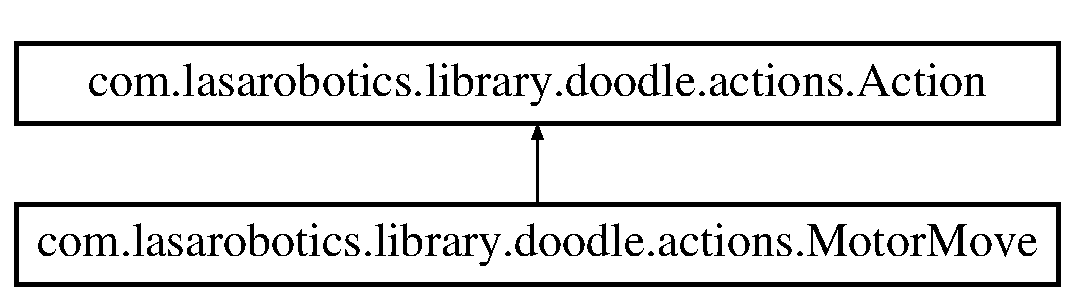
\includegraphics[height=2.000000cm]{classcom_1_1lasarobotics_1_1library_1_1doodle_1_1actions_1_1_motor_move}
\end{center}
\end{figure}
\subsection*{Public Member Functions}
\begin{DoxyCompactItemize}
\item 
\hypertarget{classcom_1_1lasarobotics_1_1library_1_1doodle_1_1actions_1_1_motor_move_aefc719748a420421f891ee0f3e9e97e4}{}{\bfseries Motor\+Move} (float power, String motor)\label{classcom_1_1lasarobotics_1_1library_1_1doodle_1_1actions_1_1_motor_move_aefc719748a420421f891ee0f3e9e97e4}

\item 
\hypertarget{classcom_1_1lasarobotics_1_1library_1_1doodle_1_1actions_1_1_motor_move_a23193548b85fb1628f6a5ea8b1431181}{}void {\bfseries run} (\hyperlink{classcom_1_1lasarobotics_1_1library_1_1doodle_1_1_doodle_run_data}{Doodle\+Run\+Data} data)\label{classcom_1_1lasarobotics_1_1library_1_1doodle_1_1actions_1_1_motor_move_a23193548b85fb1628f6a5ea8b1431181}

\item 
\hypertarget{classcom_1_1lasarobotics_1_1library_1_1doodle_1_1actions_1_1_motor_move_a34d90b5f9de699addd60a63eef16175b}{}String {\bfseries to\+String} ()\label{classcom_1_1lasarobotics_1_1library_1_1doodle_1_1actions_1_1_motor_move_a34d90b5f9de699addd60a63eef16175b}

\end{DoxyCompactItemize}
\subsection*{Additional Inherited Members}


\subsection{Detailed Description}
Move a motor at a specified power 

The documentation for this class was generated from the following file\+:\begin{DoxyCompactItemize}
\item 
ftc-\/library/src/main/java/com/lasarobotics/library/doodle/actions/Motor\+Move.\+java\end{DoxyCompactItemize}

\hypertarget{classcom_1_1lasarobotics_1_1library_1_1doodle_1_1actions_1_1_no_operation}{}\section{com.\+lasarobotics.\+library.\+doodle.\+actions.\+No\+Operation Class Reference}
\label{classcom_1_1lasarobotics_1_1library_1_1doodle_1_1actions_1_1_no_operation}\index{com.\+lasarobotics.\+library.\+doodle.\+actions.\+No\+Operation@{com.\+lasarobotics.\+library.\+doodle.\+actions.\+No\+Operation}}
Inheritance diagram for com.\+lasarobotics.\+library.\+doodle.\+actions.\+No\+Operation\+:\begin{figure}[H]
\begin{center}
\leavevmode
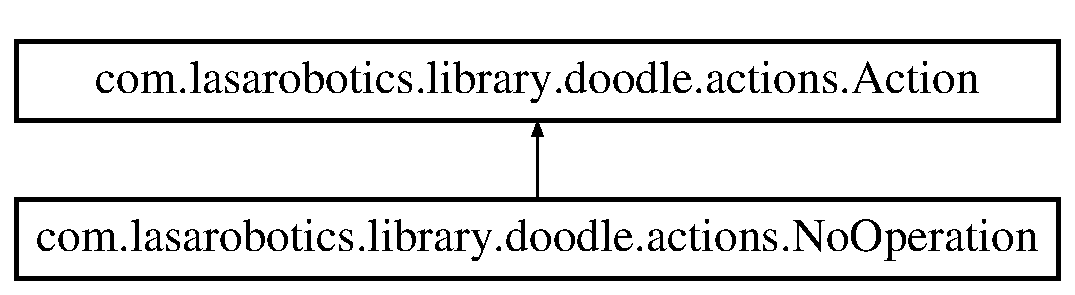
\includegraphics[height=2.000000cm]{classcom_1_1lasarobotics_1_1library_1_1doodle_1_1actions_1_1_no_operation}
\end{center}
\end{figure}
\subsection*{Public Member Functions}
\begin{DoxyCompactItemize}
\item 
\hypertarget{classcom_1_1lasarobotics_1_1library_1_1doodle_1_1actions_1_1_no_operation_a3c33ee348e3e3409d973daf966233a0a}{}void {\bfseries run} (\hyperlink{classcom_1_1lasarobotics_1_1library_1_1doodle_1_1_doodle_run_data}{Doodle\+Run\+Data} data)\label{classcom_1_1lasarobotics_1_1library_1_1doodle_1_1actions_1_1_no_operation_a3c33ee348e3e3409d973daf966233a0a}

\item 
\hypertarget{classcom_1_1lasarobotics_1_1library_1_1doodle_1_1actions_1_1_no_operation_a930ef51adf54ddd588715e30e14a06e9}{}String {\bfseries to\+String} ()\label{classcom_1_1lasarobotics_1_1library_1_1doodle_1_1actions_1_1_no_operation_a930ef51adf54ddd588715e30e14a06e9}

\end{DoxyCompactItemize}
\subsection*{Additional Inherited Members}


\subsection{Detailed Description}
Dummy action that does absolutely nothing but waste precious disk space. It\textquotesingle{}s a great starting template though. 

The documentation for this class was generated from the following file\+:\begin{DoxyCompactItemize}
\item 
ftc-\/library/src/main/java/com/lasarobotics/library/doodle/actions/No\+Operation.\+java\end{DoxyCompactItemize}

\hypertarget{classcom_1_1lasarobotics_1_1library_1_1sensor_1_1modernrobotics_1_1_optical_distance}{}\section{com.\+lasarobotics.\+library.\+sensor.\+modernrobotics.\+Optical\+Distance Class Reference}
\label{classcom_1_1lasarobotics_1_1library_1_1sensor_1_1modernrobotics_1_1_optical_distance}\index{com.\+lasarobotics.\+library.\+sensor.\+modernrobotics.\+Optical\+Distance@{com.\+lasarobotics.\+library.\+sensor.\+modernrobotics.\+Optical\+Distance}}
\subsection*{Public Member Functions}
\begin{DoxyCompactItemize}
\item 
\hypertarget{classcom_1_1lasarobotics_1_1library_1_1sensor_1_1modernrobotics_1_1_optical_distance_ad4009ff3381a553cc78787dc3932c7ac}{}{\bfseries Optical\+Distance} (Optical\+Distance\+Sensor sensor)\label{classcom_1_1lasarobotics_1_1library_1_1sensor_1_1modernrobotics_1_1_optical_distance_ad4009ff3381a553cc78787dc3932c7ac}

\item 
\hypertarget{classcom_1_1lasarobotics_1_1library_1_1sensor_1_1modernrobotics_1_1_optical_distance_ae58a79f371560087ea2d9ab2ec3f61b8}{}void {\bfseries update} (Optical\+Distance\+Sensor sensor)\label{classcom_1_1lasarobotics_1_1library_1_1sensor_1_1modernrobotics_1_1_optical_distance_ae58a79f371560087ea2d9ab2ec3f61b8}

\item 
double \hyperlink{classcom_1_1lasarobotics_1_1library_1_1sensor_1_1modernrobotics_1_1_optical_distance_a0694b6194e93fb22bcebeb0aff66486b}{get\+Light\+Detected} ()
\item 
Boolean \hyperlink{classcom_1_1lasarobotics_1_1library_1_1sensor_1_1modernrobotics_1_1_optical_distance_a366a12fd4ccfb876a22464b4c6096899}{object\+Detected} ()
\item 
Boolean \hyperlink{classcom_1_1lasarobotics_1_1library_1_1sensor_1_1modernrobotics_1_1_optical_distance_ab77075ad6e8a0523a6f77b7fbc54a2da}{object\+Near} ()
\item 
Boolean \hyperlink{classcom_1_1lasarobotics_1_1library_1_1sensor_1_1modernrobotics_1_1_optical_distance_ac3d175c6bfb8bbcb8abb50e2febbe6fc}{object\+Close} ()
\item 
double \hyperlink{classcom_1_1lasarobotics_1_1library_1_1sensor_1_1modernrobotics_1_1_optical_distance_afc702503dd61db5ae033af322a474cf9}{get\+Distance} ()
\end{DoxyCompactItemize}


\subsection{Detailed Description}
Implements the Core Optical \hyperlink{classcom_1_1lasarobotics_1_1library_1_1sensor_1_1modernrobotics_1_1_optical_distance}{Optical\+Distance} Sensor with advanced methods

This sensor is only fully accurate U\+P T\+O 5 C\+M Different lighting conditions greatly affect distance read after 5 cm away from the object 

\subsection{Member Function Documentation}
\hypertarget{classcom_1_1lasarobotics_1_1library_1_1sensor_1_1modernrobotics_1_1_optical_distance_afc702503dd61db5ae033af322a474cf9}{}\index{com\+::lasarobotics\+::library\+::sensor\+::modernrobotics\+::\+Optical\+Distance@{com\+::lasarobotics\+::library\+::sensor\+::modernrobotics\+::\+Optical\+Distance}!get\+Distance@{get\+Distance}}
\index{get\+Distance@{get\+Distance}!com\+::lasarobotics\+::library\+::sensor\+::modernrobotics\+::\+Optical\+Distance@{com\+::lasarobotics\+::library\+::sensor\+::modernrobotics\+::\+Optical\+Distance}}
\subsubsection[{get\+Distance()}]{\setlength{\rightskip}{0pt plus 5cm}double com.\+lasarobotics.\+library.\+sensor.\+modernrobotics.\+Optical\+Distance.\+get\+Distance (
\begin{DoxyParamCaption}
{}
\end{DoxyParamCaption}
)}\label{classcom_1_1lasarobotics_1_1library_1_1sensor_1_1modernrobotics_1_1_optical_distance_afc702503dd61db5ae033af322a474cf9}
Gets an approximate distance from the object in centimeters Formula based on empirical measurements in 2700\+K lighting at room temperature with a white semi-\/reflective object perpendicular to the beam

Please note that these values are only S\+O\+M\+E\+W\+H\+A\+T A\+C\+C\+U\+R\+A\+T\+E between 0.\+5 and 5 cm! \begin{DoxyReturn}{Returns}
An approximate distance in centimeters 
\end{DoxyReturn}
\hypertarget{classcom_1_1lasarobotics_1_1library_1_1sensor_1_1modernrobotics_1_1_optical_distance_a0694b6194e93fb22bcebeb0aff66486b}{}\index{com\+::lasarobotics\+::library\+::sensor\+::modernrobotics\+::\+Optical\+Distance@{com\+::lasarobotics\+::library\+::sensor\+::modernrobotics\+::\+Optical\+Distance}!get\+Light\+Detected@{get\+Light\+Detected}}
\index{get\+Light\+Detected@{get\+Light\+Detected}!com\+::lasarobotics\+::library\+::sensor\+::modernrobotics\+::\+Optical\+Distance@{com\+::lasarobotics\+::library\+::sensor\+::modernrobotics\+::\+Optical\+Distance}}
\subsubsection[{get\+Light\+Detected()}]{\setlength{\rightskip}{0pt plus 5cm}double com.\+lasarobotics.\+library.\+sensor.\+modernrobotics.\+Optical\+Distance.\+get\+Light\+Detected (
\begin{DoxyParamCaption}
{}
\end{DoxyParamCaption}
)}\label{classcom_1_1lasarobotics_1_1library_1_1sensor_1_1modernrobotics_1_1_optical_distance_a0694b6194e93fb22bcebeb0aff66486b}
Gets the raw light reflected as a decimal \begin{DoxyReturn}{Returns}
The raw light reflected as a decimal 
\end{DoxyReturn}
\hypertarget{classcom_1_1lasarobotics_1_1library_1_1sensor_1_1modernrobotics_1_1_optical_distance_ac3d175c6bfb8bbcb8abb50e2febbe6fc}{}\index{com\+::lasarobotics\+::library\+::sensor\+::modernrobotics\+::\+Optical\+Distance@{com\+::lasarobotics\+::library\+::sensor\+::modernrobotics\+::\+Optical\+Distance}!object\+Close@{object\+Close}}
\index{object\+Close@{object\+Close}!com\+::lasarobotics\+::library\+::sensor\+::modernrobotics\+::\+Optical\+Distance@{com\+::lasarobotics\+::library\+::sensor\+::modernrobotics\+::\+Optical\+Distance}}
\subsubsection[{object\+Close()}]{\setlength{\rightskip}{0pt plus 5cm}Boolean com.\+lasarobotics.\+library.\+sensor.\+modernrobotics.\+Optical\+Distance.\+object\+Close (
\begin{DoxyParamCaption}
{}
\end{DoxyParamCaption}
)}\label{classcom_1_1lasarobotics_1_1library_1_1sensor_1_1modernrobotics_1_1_optical_distance_ac3d175c6bfb8bbcb8abb50e2febbe6fc}
Returns true if an object is close enough to get an accurate distance measurement of +-\/ 1 cm, assuming light object \begin{DoxyReturn}{Returns}
True if an object is close enough to get an accurate distance measurement 
\end{DoxyReturn}
\hypertarget{classcom_1_1lasarobotics_1_1library_1_1sensor_1_1modernrobotics_1_1_optical_distance_a366a12fd4ccfb876a22464b4c6096899}{}\index{com\+::lasarobotics\+::library\+::sensor\+::modernrobotics\+::\+Optical\+Distance@{com\+::lasarobotics\+::library\+::sensor\+::modernrobotics\+::\+Optical\+Distance}!object\+Detected@{object\+Detected}}
\index{object\+Detected@{object\+Detected}!com\+::lasarobotics\+::library\+::sensor\+::modernrobotics\+::\+Optical\+Distance@{com\+::lasarobotics\+::library\+::sensor\+::modernrobotics\+::\+Optical\+Distance}}
\subsubsection[{object\+Detected()}]{\setlength{\rightskip}{0pt plus 5cm}Boolean com.\+lasarobotics.\+library.\+sensor.\+modernrobotics.\+Optical\+Distance.\+object\+Detected (
\begin{DoxyParamCaption}
{}
\end{DoxyParamCaption}
)}\label{classcom_1_1lasarobotics_1_1library_1_1sensor_1_1modernrobotics_1_1_optical_distance_a366a12fd4ccfb876a22464b4c6096899}
Returns true if an object is detected within the sensor\textquotesingle{}s absolute maximum range (25 cm) \begin{DoxyReturn}{Returns}
True if an object is detected 
\end{DoxyReturn}
\hypertarget{classcom_1_1lasarobotics_1_1library_1_1sensor_1_1modernrobotics_1_1_optical_distance_ab77075ad6e8a0523a6f77b7fbc54a2da}{}\index{com\+::lasarobotics\+::library\+::sensor\+::modernrobotics\+::\+Optical\+Distance@{com\+::lasarobotics\+::library\+::sensor\+::modernrobotics\+::\+Optical\+Distance}!object\+Near@{object\+Near}}
\index{object\+Near@{object\+Near}!com\+::lasarobotics\+::library\+::sensor\+::modernrobotics\+::\+Optical\+Distance@{com\+::lasarobotics\+::library\+::sensor\+::modernrobotics\+::\+Optical\+Distance}}
\subsubsection[{object\+Near()}]{\setlength{\rightskip}{0pt plus 5cm}Boolean com.\+lasarobotics.\+library.\+sensor.\+modernrobotics.\+Optical\+Distance.\+object\+Near (
\begin{DoxyParamCaption}
{}
\end{DoxyParamCaption}
)}\label{classcom_1_1lasarobotics_1_1library_1_1sensor_1_1modernrobotics_1_1_optical_distance_ab77075ad6e8a0523a6f77b7fbc54a2da}
Returns true if an object is near the sensor (within 5-\/10 cm) \begin{DoxyReturn}{Returns}
True if an object is near the sensor 
\end{DoxyReturn}


The documentation for this class was generated from the following file\+:\begin{DoxyCompactItemize}
\item 
ftc-\/library/src/main/java/com/lasarobotics/library/sensor/modernrobotics/Optical\+Distance.\+java\end{DoxyCompactItemize}

\hypertarget{enumcom_1_1lasarobotics_1_1library_1_1doodle_1_1maps_1_1_doodle_map_1_1_range_of_motion}{}\section{com.\+lasarobotics.\+library.\+doodle.\+maps.\+Doodle\+Map.\+Range\+Of\+Motion Enum Reference}
\label{enumcom_1_1lasarobotics_1_1library_1_1doodle_1_1maps_1_1_doodle_map_1_1_range_of_motion}\index{com.\+lasarobotics.\+library.\+doodle.\+maps.\+Doodle\+Map.\+Range\+Of\+Motion@{com.\+lasarobotics.\+library.\+doodle.\+maps.\+Doodle\+Map.\+Range\+Of\+Motion}}
\subsection*{Public Attributes}
\begin{DoxyCompactItemize}
\item 
\hypertarget{enumcom_1_1lasarobotics_1_1library_1_1doodle_1_1maps_1_1_doodle_map_1_1_range_of_motion_a1601259e5d1d3ba6b589fa7047b5f1db}{}{\bfseries D\+R\+I\+V\+E\+\_\+\+A\+M\+P\+L\+I\+T\+U\+D\+E\+\_\+\+O\+N\+L\+Y}\label{enumcom_1_1lasarobotics_1_1library_1_1doodle_1_1maps_1_1_doodle_map_1_1_range_of_motion_a1601259e5d1d3ba6b589fa7047b5f1db}

\item 
\hypertarget{enumcom_1_1lasarobotics_1_1library_1_1doodle_1_1maps_1_1_doodle_map_1_1_range_of_motion_a4fdbab7e6d4c4b0a7527668096bc23e0}{}{\bfseries D\+R\+I\+V\+E\+\_\+\+A\+M\+P\+L\+I\+T\+U\+D\+E\+\_\+\+R\+O\+T\+A\+T\+I\+O\+N}\label{enumcom_1_1lasarobotics_1_1library_1_1doodle_1_1maps_1_1_doodle_map_1_1_range_of_motion_a4fdbab7e6d4c4b0a7527668096bc23e0}

\end{DoxyCompactItemize}


The documentation for this enum was generated from the following file\+:\begin{DoxyCompactItemize}
\item 
ftc-\/library/src/main/java/com/lasarobotics/library/doodle/maps/Doodle\+Map.\+java\end{DoxyCompactItemize}

\hypertarget{classcom_1_1lasarobotics_1_1library_1_1util_1_1_rolling_average}{}\section{com.\+lasarobotics.\+library.\+util.\+Rolling\+Average$<$ T extends Number $>$ Class Template Reference}
\label{classcom_1_1lasarobotics_1_1library_1_1util_1_1_rolling_average}\index{com.\+lasarobotics.\+library.\+util.\+Rolling\+Average$<$ T extends Number $>$@{com.\+lasarobotics.\+library.\+util.\+Rolling\+Average$<$ T extends Number $>$}}
\subsection*{Public Member Functions}
\begin{DoxyCompactItemize}
\item 
\hypertarget{classcom_1_1lasarobotics_1_1library_1_1util_1_1_rolling_average_ae431f75889ba3375b3a852be00e5b007}{}{\bfseries Rolling\+Average} (int capacity)\label{classcom_1_1lasarobotics_1_1library_1_1util_1_1_rolling_average_ae431f75889ba3375b3a852be00e5b007}

\item 
\hypertarget{classcom_1_1lasarobotics_1_1library_1_1util_1_1_rolling_average_a3cae7fa9489d73c1c1f981ad4008ea22}{}void {\bfseries add\+Value} (T value)\label{classcom_1_1lasarobotics_1_1library_1_1util_1_1_rolling_average_a3cae7fa9489d73c1c1f981ad4008ea22}

\item 
\hypertarget{classcom_1_1lasarobotics_1_1library_1_1util_1_1_rolling_average_af8ddaee994f8a4ef950d3ae346d577db}{}int {\bfseries get\+Capacity} ()\label{classcom_1_1lasarobotics_1_1library_1_1util_1_1_rolling_average_af8ddaee994f8a4ef950d3ae346d577db}

\item 
\hypertarget{classcom_1_1lasarobotics_1_1library_1_1util_1_1_rolling_average_afa65f13150c305f83f5b66b34ba073a4}{}void {\bfseries set\+Capacity} (int capacity)\label{classcom_1_1lasarobotics_1_1library_1_1util_1_1_rolling_average_afa65f13150c305f83f5b66b34ba073a4}

\item 
\hypertarget{classcom_1_1lasarobotics_1_1library_1_1util_1_1_rolling_average_abe3e09c5a64f209c350b0ee755208ac1}{}void {\bfseries clear} ()\label{classcom_1_1lasarobotics_1_1library_1_1util_1_1_rolling_average_abe3e09c5a64f209c350b0ee755208ac1}

\item 
\hypertarget{classcom_1_1lasarobotics_1_1library_1_1util_1_1_rolling_average_a20361639d89c2447bd3eeee92035a9b3}{}int {\bfseries get\+Size} ()\label{classcom_1_1lasarobotics_1_1library_1_1util_1_1_rolling_average_a20361639d89c2447bd3eeee92035a9b3}

\item 
\hypertarget{classcom_1_1lasarobotics_1_1library_1_1util_1_1_rolling_average_a227073b1b13ce0a4835623ebebfa4438}{}double {\bfseries get\+Average} ()\label{classcom_1_1lasarobotics_1_1library_1_1util_1_1_rolling_average_a227073b1b13ce0a4835623ebebfa4438}

\item 
\hypertarget{classcom_1_1lasarobotics_1_1library_1_1util_1_1_rolling_average_a0402a4b403f9f8af9781115568c12813}{}double {\bfseries get\+Total} ()\label{classcom_1_1lasarobotics_1_1library_1_1util_1_1_rolling_average_a0402a4b403f9f8af9781115568c12813}

\end{DoxyCompactItemize}


\subsection{Detailed Description}
Structure that performs a continuous rolling average on values Uses doubles as internal structures 

The documentation for this class was generated from the following file\+:\begin{DoxyCompactItemize}
\item 
ftc-\/library/src/main/java/com/lasarobotics/library/util/Rolling\+Average.\+java\end{DoxyCompactItemize}

\hypertarget{classcom_1_1lasarobotics_1_1library_1_1sensor_1_1android_1_1_sensors}{}\section{com.\+lasarobotics.\+library.\+sensor.\+android.\+Sensors Class Reference}
\label{classcom_1_1lasarobotics_1_1library_1_1sensor_1_1android_1_1_sensors}\index{com.\+lasarobotics.\+library.\+sensor.\+android.\+Sensors@{com.\+lasarobotics.\+library.\+sensor.\+android.\+Sensors}}
\subsection*{Static Public Member Functions}
\begin{DoxyCompactItemize}
\item 
\hypertarget{classcom_1_1lasarobotics_1_1library_1_1sensor_1_1android_1_1_sensors_a632da87e087bc969fd237ffebea49ff4}{}static List$<$ Sensor $>$ {\bfseries get\+All\+Sensors} ()\label{classcom_1_1lasarobotics_1_1library_1_1sensor_1_1android_1_1_sensors_a632da87e087bc969fd237ffebea49ff4}

\item 
\hypertarget{classcom_1_1lasarobotics_1_1library_1_1sensor_1_1android_1_1_sensors_abf64e300cb51466da078c1c952a8c818}{}static Sensor {\bfseries get\+Sensor} (int type)\label{classcom_1_1lasarobotics_1_1library_1_1sensor_1_1android_1_1_sensors_abf64e300cb51466da078c1c952a8c818}

\item 
\hypertarget{classcom_1_1lasarobotics_1_1library_1_1sensor_1_1android_1_1_sensors_a9e9eccb5e01be00865871b97fb899cd3}{}static Boolean {\bfseries has\+Sensor} (int type)\label{classcom_1_1lasarobotics_1_1library_1_1sensor_1_1android_1_1_sensors_a9e9eccb5e01be00865871b97fb899cd3}

\end{DoxyCompactItemize}


\subsection{Detailed Description}
Lists Android manager, converts manager to this library\textquotesingle{}s format, and tests if certain sensor is present

Use for any Android internal device sensor implemented in hardware O\+R software 

The documentation for this class was generated from the following file\+:\begin{DoxyCompactItemize}
\item 
ftc-\/library/src/main/java/com/lasarobotics/library/sensor/android/Sensors.\+java\end{DoxyCompactItemize}

\hypertarget{classcom_1_1lasarobotics_1_1library_1_1drive_1_1_swerve}{}\section{com.\+lasarobotics.\+library.\+drive.\+Swerve Class Reference}
\label{classcom_1_1lasarobotics_1_1library_1_1drive_1_1_swerve}\index{com.\+lasarobotics.\+library.\+drive.\+Swerve@{com.\+lasarobotics.\+library.\+drive.\+Swerve}}
\subsection*{Static Public Member Functions}
\begin{DoxyCompactItemize}
\item 
static void \hyperlink{classcom_1_1lasarobotics_1_1library_1_1drive_1_1_swerve_a5fb0f43c7fbdfc9fef6a1f5af9848e0a}{Standard} (double y, double x, double rot, double gyroheading, Dc\+Motor left\+Front, Dc\+Motor right\+Front, Dc\+Motor left\+Back, Dc\+Motor right\+Back, Servo lf, Servo rf, Servo lb, Servo rb)
\end{DoxyCompactItemize}


\subsection{Detailed Description}
Methods for the \hyperlink{classcom_1_1lasarobotics_1_1library_1_1drive_1_1_swerve}{Swerve} drive train 

\subsection{Member Function Documentation}
\hypertarget{classcom_1_1lasarobotics_1_1library_1_1drive_1_1_swerve_a5fb0f43c7fbdfc9fef6a1f5af9848e0a}{}\index{com\+::lasarobotics\+::library\+::drive\+::\+Swerve@{com\+::lasarobotics\+::library\+::drive\+::\+Swerve}!Standard@{Standard}}
\index{Standard@{Standard}!com\+::lasarobotics\+::library\+::drive\+::\+Swerve@{com\+::lasarobotics\+::library\+::drive\+::\+Swerve}}
\subsubsection[{Standard(double y, double x, double rot, double gyroheading, Dc\+Motor left\+Front, Dc\+Motor right\+Front, Dc\+Motor left\+Back, Dc\+Motor right\+Back, Servo lf, Servo rf, Servo lb, Servo rb)}]{\setlength{\rightskip}{0pt plus 5cm}static void com.\+lasarobotics.\+library.\+drive.\+Swerve.\+Standard (
\begin{DoxyParamCaption}
\item[{double}]{y, }
\item[{double}]{x, }
\item[{double}]{rot, }
\item[{double}]{gyroheading, }
\item[{Dc\+Motor}]{left\+Front, }
\item[{Dc\+Motor}]{right\+Front, }
\item[{Dc\+Motor}]{left\+Back, }
\item[{Dc\+Motor}]{right\+Back, }
\item[{Servo}]{lf, }
\item[{Servo}]{rf, }
\item[{Servo}]{lb, }
\item[{Servo}]{rb}
\end{DoxyParamCaption}
)\hspace{0.3cm}{\ttfamily [static]}}\label{classcom_1_1lasarobotics_1_1library_1_1drive_1_1_swerve_a5fb0f43c7fbdfc9fef6a1f5af9848e0a}
Implements the \hyperlink{classcom_1_1lasarobotics_1_1library_1_1drive_1_1_swerve}{Swerve} drive train with four motors and four lifting servos Requires gyro input


\begin{DoxyParams}{Parameters}
{\em y} & The y-\/axis of the controller, forward/rev \\
\hline
{\em x} & The x-\/axis of the controller, strafe \\
\hline
{\em rot} & The spin axis of the controller \\
\hline
{\em gyroheading} & The current normalized gyro heading (between 0 and 360) \\
\hline
{\em left\+Front} & The motor on the front left \\
\hline
{\em right\+Front} & The motor on the front right \\
\hline
{\em left\+Back} & The motor on the back left \\
\hline
{\em right\+Back} & The motor on the back right \\
\hline
{\em lf} & The servo on the front left \\
\hline
{\em rf} & The servo on the front right \\
\hline
{\em lb} & The servo on the back left \\
\hline
{\em rb} & The servo on the back right \\
\hline
\end{DoxyParams}


The documentation for this class was generated from the following file\+:\begin{DoxyCompactItemize}
\item 
ftc-\/library/src/main/java/com/lasarobotics/library/drive/Swerve.\+java\end{DoxyCompactItemize}

\hypertarget{classcom_1_1lasarobotics_1_1library_1_1drive_1_1_tank}{}\section{com.\+lasarobotics.\+library.\+drive.\+Tank Class Reference}
\label{classcom_1_1lasarobotics_1_1library_1_1drive_1_1_tank}\index{com.\+lasarobotics.\+library.\+drive.\+Tank@{com.\+lasarobotics.\+library.\+drive.\+Tank}}
\subsection*{Static Public Member Functions}
\begin{DoxyCompactItemize}
\item 
static void \hyperlink{classcom_1_1lasarobotics_1_1library_1_1drive_1_1_tank_ad00f8c122db08fdf3399e10a50dabede}{Motor2} (Dc\+Motor left, Dc\+Motor right, double left\+Value, double right\+Value)
\item 
static void \hyperlink{classcom_1_1lasarobotics_1_1library_1_1drive_1_1_tank_a49450548769799647ee538ea4e8a7d01}{Motor4} (Dc\+Motor left\+Front, Dc\+Motor right\+Front, Dc\+Motor left\+Back, Dc\+Motor right\+Back, double left\+Value, double right\+Value)
\end{DoxyCompactItemize}


\subsection{Detailed Description}
Methods for the \hyperlink{classcom_1_1lasarobotics_1_1library_1_1drive_1_1_tank}{Tank} drive train. 

\subsection{Member Function Documentation}
\hypertarget{classcom_1_1lasarobotics_1_1library_1_1drive_1_1_tank_ad00f8c122db08fdf3399e10a50dabede}{}\index{com\+::lasarobotics\+::library\+::drive\+::\+Tank@{com\+::lasarobotics\+::library\+::drive\+::\+Tank}!Motor2@{Motor2}}
\index{Motor2@{Motor2}!com\+::lasarobotics\+::library\+::drive\+::\+Tank@{com\+::lasarobotics\+::library\+::drive\+::\+Tank}}
\subsubsection[{Motor2(\+Dc\+Motor left, Dc\+Motor right, double left\+Value, double right\+Value)}]{\setlength{\rightskip}{0pt plus 5cm}static void com.\+lasarobotics.\+library.\+drive.\+Tank.\+Motor2 (
\begin{DoxyParamCaption}
\item[{Dc\+Motor}]{left, }
\item[{Dc\+Motor}]{right, }
\item[{double}]{left\+Value, }
\item[{double}]{right\+Value}
\end{DoxyParamCaption}
)\hspace{0.3cm}{\ttfamily [static]}}\label{classcom_1_1lasarobotics_1_1library_1_1drive_1_1_tank_ad00f8c122db08fdf3399e10a50dabede}
Implements the \hyperlink{classcom_1_1lasarobotics_1_1library_1_1drive_1_1_tank}{Tank} drive train with two motors 
\begin{DoxyParams}{Parameters}
{\em left} & Left motor \\
\hline
{\em right} & Right motor \\
\hline
{\em left\+Value} & Left motor target value \\
\hline
{\em right\+Value} & Right motor target value \\
\hline
\end{DoxyParams}
\hypertarget{classcom_1_1lasarobotics_1_1library_1_1drive_1_1_tank_a49450548769799647ee538ea4e8a7d01}{}\index{com\+::lasarobotics\+::library\+::drive\+::\+Tank@{com\+::lasarobotics\+::library\+::drive\+::\+Tank}!Motor4@{Motor4}}
\index{Motor4@{Motor4}!com\+::lasarobotics\+::library\+::drive\+::\+Tank@{com\+::lasarobotics\+::library\+::drive\+::\+Tank}}
\subsubsection[{Motor4(\+Dc\+Motor left\+Front, Dc\+Motor right\+Front, Dc\+Motor left\+Back, Dc\+Motor right\+Back, double left\+Value, double right\+Value)}]{\setlength{\rightskip}{0pt plus 5cm}static void com.\+lasarobotics.\+library.\+drive.\+Tank.\+Motor4 (
\begin{DoxyParamCaption}
\item[{Dc\+Motor}]{left\+Front, }
\item[{Dc\+Motor}]{right\+Front, }
\item[{Dc\+Motor}]{left\+Back, }
\item[{Dc\+Motor}]{right\+Back, }
\item[{double}]{left\+Value, }
\item[{double}]{right\+Value}
\end{DoxyParamCaption}
)\hspace{0.3cm}{\ttfamily [static]}}\label{classcom_1_1lasarobotics_1_1library_1_1drive_1_1_tank_a49450548769799647ee538ea4e8a7d01}
Implements the \hyperlink{classcom_1_1lasarobotics_1_1library_1_1drive_1_1_tank}{Tank} drive train with four motors 
\begin{DoxyParams}{Parameters}
{\em left\+Front} & The motor on the front left \\
\hline
{\em right\+Front} & The motor on the front right \\
\hline
{\em left\+Back} & The motor on the back left \\
\hline
{\em right\+Back} & The motor on the back right \\
\hline
{\em left\+Value} & Left motors target value \\
\hline
{\em right\+Value} & Right motors target value \\
\hline
\end{DoxyParams}


The documentation for this class was generated from the following file\+:\begin{DoxyCompactItemize}
\item 
ftc-\/library/src/main/java/com/lasarobotics/library/drive/Tank.\+java\end{DoxyCompactItemize}

\hypertarget{classcom_1_1lasarobotics_1_1library_1_1util_1_1_timers}{}\section{com.\+lasarobotics.\+library.\+util.\+Timers Class Reference}
\label{classcom_1_1lasarobotics_1_1library_1_1util_1_1_timers}\index{com.\+lasarobotics.\+library.\+util.\+Timers@{com.\+lasarobotics.\+library.\+util.\+Timers}}
\subsection*{Public Member Functions}
\begin{DoxyCompactItemize}
\item 
\hyperlink{classcom_1_1lasarobotics_1_1library_1_1util_1_1_timers_a05e3526671638c8a7989faa021972a5a}{Timers} ()
\item 
\hyperlink{classcom_1_1lasarobotics_1_1library_1_1util_1_1_timers_a85a3d0fdaaf25c38a0f0cf8f8a3270ae}{Timers} (int precision)
\item 
void \hyperlink{classcom_1_1lasarobotics_1_1library_1_1util_1_1_timers_a0baeaa0b504aae6298341e4e4258f41c}{start\+Clock} (String name)
\item 
void \hyperlink{classcom_1_1lasarobotics_1_1library_1_1util_1_1_timers_adfd15587ecf606bc5edd2484be56047a}{reset\+Clock} (String name)
\item 
long \hyperlink{classcom_1_1lasarobotics_1_1library_1_1util_1_1_timers_a7e981eca3d9a4ae24e08a56f375a74cc}{get\+Clock\+Value} (String name)
\item 
long \hyperlink{classcom_1_1lasarobotics_1_1library_1_1util_1_1_timers_afc579ae87fe551fbf34b35bc0ffd0ba6}{get\+Clock\+Value} (String name, Time\+Unit time\+Unit)
\item 
boolean \hyperlink{classcom_1_1lasarobotics_1_1library_1_1util_1_1_timers_a18f1e196191869904f1bf68158929dcf}{is\+At\+Target\+Millis} (String name, long target)
\item 
boolean \hyperlink{classcom_1_1lasarobotics_1_1library_1_1util_1_1_timers_a5cd21a3b007ee957507830fabb952dfd}{is\+At\+Target\+Millis} (String name, long target, long precision)
\item 
long \hyperlink{classcom_1_1lasarobotics_1_1library_1_1util_1_1_timers_a6c7fcedc038f1e8b9f8e0cd6bfdce308}{get\+Precision} ()
\item 
void \hyperlink{classcom_1_1lasarobotics_1_1library_1_1util_1_1_timers_a9bc557ec5fbf399594df81d132e3b46f}{set\+Precision} (int precision)
\end{DoxyCompactItemize}


\subsection{Detailed Description}
Implements advanced timers with events and precision manipulation. 

\subsection{Constructor \& Destructor Documentation}
\hypertarget{classcom_1_1lasarobotics_1_1library_1_1util_1_1_timers_a05e3526671638c8a7989faa021972a5a}{}\index{com\+::lasarobotics\+::library\+::util\+::\+Timers@{com\+::lasarobotics\+::library\+::util\+::\+Timers}!Timers@{Timers}}
\index{Timers@{Timers}!com\+::lasarobotics\+::library\+::util\+::\+Timers@{com\+::lasarobotics\+::library\+::util\+::\+Timers}}
\subsubsection[{Timers()}]{\setlength{\rightskip}{0pt plus 5cm}com.\+lasarobotics.\+library.\+util.\+Timers.\+Timers (
\begin{DoxyParamCaption}
{}
\end{DoxyParamCaption}
)}\label{classcom_1_1lasarobotics_1_1library_1_1util_1_1_timers_a05e3526671638c8a7989faa021972a5a}
Instantiates the timer class with the default millisecond precision. \hypertarget{classcom_1_1lasarobotics_1_1library_1_1util_1_1_timers_a85a3d0fdaaf25c38a0f0cf8f8a3270ae}{}\index{com\+::lasarobotics\+::library\+::util\+::\+Timers@{com\+::lasarobotics\+::library\+::util\+::\+Timers}!Timers@{Timers}}
\index{Timers@{Timers}!com\+::lasarobotics\+::library\+::util\+::\+Timers@{com\+::lasarobotics\+::library\+::util\+::\+Timers}}
\subsubsection[{Timers(int precision)}]{\setlength{\rightskip}{0pt plus 5cm}com.\+lasarobotics.\+library.\+util.\+Timers.\+Timers (
\begin{DoxyParamCaption}
\item[{int}]{precision}
\end{DoxyParamCaption}
)}\label{classcom_1_1lasarobotics_1_1library_1_1util_1_1_timers_a85a3d0fdaaf25c38a0f0cf8f8a3270ae}
Instantiates the timer class with an arbitrary precision in milliseconds. 
\begin{DoxyParams}{Parameters}
{\em precision} & Precision of the clock, in milliseconds. \\
\hline
\end{DoxyParams}


\subsection{Member Function Documentation}
\hypertarget{classcom_1_1lasarobotics_1_1library_1_1util_1_1_timers_a7e981eca3d9a4ae24e08a56f375a74cc}{}\index{com\+::lasarobotics\+::library\+::util\+::\+Timers@{com\+::lasarobotics\+::library\+::util\+::\+Timers}!get\+Clock\+Value@{get\+Clock\+Value}}
\index{get\+Clock\+Value@{get\+Clock\+Value}!com\+::lasarobotics\+::library\+::util\+::\+Timers@{com\+::lasarobotics\+::library\+::util\+::\+Timers}}
\subsubsection[{get\+Clock\+Value(\+String name)}]{\setlength{\rightskip}{0pt plus 5cm}long com.\+lasarobotics.\+library.\+util.\+Timers.\+get\+Clock\+Value (
\begin{DoxyParamCaption}
\item[{String}]{name}
\end{DoxyParamCaption}
)}\label{classcom_1_1lasarobotics_1_1library_1_1util_1_1_timers_a7e981eca3d9a4ae24e08a56f375a74cc}
Get clock value. Defaults to millisecond precision. 
\begin{DoxyParams}{Parameters}
{\em name} & Name of the clock \\
\hline
\end{DoxyParams}
\begin{DoxyReturn}{Returns}
Value of clock in milliseconds 
\end{DoxyReturn}
\hypertarget{classcom_1_1lasarobotics_1_1library_1_1util_1_1_timers_afc579ae87fe551fbf34b35bc0ffd0ba6}{}\index{com\+::lasarobotics\+::library\+::util\+::\+Timers@{com\+::lasarobotics\+::library\+::util\+::\+Timers}!get\+Clock\+Value@{get\+Clock\+Value}}
\index{get\+Clock\+Value@{get\+Clock\+Value}!com\+::lasarobotics\+::library\+::util\+::\+Timers@{com\+::lasarobotics\+::library\+::util\+::\+Timers}}
\subsubsection[{get\+Clock\+Value(\+String name, Time\+Unit time\+Unit)}]{\setlength{\rightskip}{0pt plus 5cm}long com.\+lasarobotics.\+library.\+util.\+Timers.\+get\+Clock\+Value (
\begin{DoxyParamCaption}
\item[{String}]{name, }
\item[{Time\+Unit}]{time\+Unit}
\end{DoxyParamCaption}
)}\label{classcom_1_1lasarobotics_1_1library_1_1util_1_1_timers_afc579ae87fe551fbf34b35bc0ffd0ba6}
Get clock value with precision in a given time unit 
\begin{DoxyParams}{Parameters}
{\em name} & Name of the clock \\
\hline
{\em time\+Unit} & Time\+Unit the output should be in \\
\hline
\end{DoxyParams}
\begin{DoxyReturn}{Returns}
The value of the clock converted to the time unit specified (may lose precision) 
\end{DoxyReturn}
\hypertarget{classcom_1_1lasarobotics_1_1library_1_1util_1_1_timers_a6c7fcedc038f1e8b9f8e0cd6bfdce308}{}\index{com\+::lasarobotics\+::library\+::util\+::\+Timers@{com\+::lasarobotics\+::library\+::util\+::\+Timers}!get\+Precision@{get\+Precision}}
\index{get\+Precision@{get\+Precision}!com\+::lasarobotics\+::library\+::util\+::\+Timers@{com\+::lasarobotics\+::library\+::util\+::\+Timers}}
\subsubsection[{get\+Precision()}]{\setlength{\rightskip}{0pt plus 5cm}long com.\+lasarobotics.\+library.\+util.\+Timers.\+get\+Precision (
\begin{DoxyParamCaption}
{}
\end{DoxyParamCaption}
)}\label{classcom_1_1lasarobotics_1_1library_1_1util_1_1_timers_a6c7fcedc038f1e8b9f8e0cd6bfdce308}
Gets the precision in milliseconds \begin{DoxyReturn}{Returns}
Precision in milliseconds 
\end{DoxyReturn}
\hypertarget{classcom_1_1lasarobotics_1_1library_1_1util_1_1_timers_a18f1e196191869904f1bf68158929dcf}{}\index{com\+::lasarobotics\+::library\+::util\+::\+Timers@{com\+::lasarobotics\+::library\+::util\+::\+Timers}!is\+At\+Target\+Millis@{is\+At\+Target\+Millis}}
\index{is\+At\+Target\+Millis@{is\+At\+Target\+Millis}!com\+::lasarobotics\+::library\+::util\+::\+Timers@{com\+::lasarobotics\+::library\+::util\+::\+Timers}}
\subsubsection[{is\+At\+Target\+Millis(\+String name, long target)}]{\setlength{\rightskip}{0pt plus 5cm}boolean com.\+lasarobotics.\+library.\+util.\+Timers.\+is\+At\+Target\+Millis (
\begin{DoxyParamCaption}
\item[{String}]{name, }
\item[{long}]{target}
\end{DoxyParamCaption}
)}\label{classcom_1_1lasarobotics_1_1library_1_1util_1_1_timers_a18f1e196191869904f1bf68158929dcf}
Returns whether the clock is at the specified amount of milliseconds 
\begin{DoxyParams}{Parameters}
{\em name} & The clock name \\
\hline
{\em target} & The target time in milliseconds \\
\hline
\end{DoxyParams}
\begin{DoxyReturn}{Returns}
True if at the target (+-\/ precision), false otherwise 
\end{DoxyReturn}
\hypertarget{classcom_1_1lasarobotics_1_1library_1_1util_1_1_timers_a5cd21a3b007ee957507830fabb952dfd}{}\index{com\+::lasarobotics\+::library\+::util\+::\+Timers@{com\+::lasarobotics\+::library\+::util\+::\+Timers}!is\+At\+Target\+Millis@{is\+At\+Target\+Millis}}
\index{is\+At\+Target\+Millis@{is\+At\+Target\+Millis}!com\+::lasarobotics\+::library\+::util\+::\+Timers@{com\+::lasarobotics\+::library\+::util\+::\+Timers}}
\subsubsection[{is\+At\+Target\+Millis(\+String name, long target, long precision)}]{\setlength{\rightskip}{0pt plus 5cm}boolean com.\+lasarobotics.\+library.\+util.\+Timers.\+is\+At\+Target\+Millis (
\begin{DoxyParamCaption}
\item[{String}]{name, }
\item[{long}]{target, }
\item[{long}]{precision}
\end{DoxyParamCaption}
)}\label{classcom_1_1lasarobotics_1_1library_1_1util_1_1_timers_a5cd21a3b007ee957507830fabb952dfd}
Returns whether the clock is at the specified amount of milliseconds 
\begin{DoxyParams}{Parameters}
{\em name} & The clock name \\
\hline
{\em target} & The target time in milliseconds \\
\hline
{\em precision} & How much target and clock value can differ by in milliseconds \\
\hline
\end{DoxyParams}
\begin{DoxyReturn}{Returns}
True if at the target (+-\/ precision), false otherwise 
\end{DoxyReturn}
\hypertarget{classcom_1_1lasarobotics_1_1library_1_1util_1_1_timers_adfd15587ecf606bc5edd2484be56047a}{}\index{com\+::lasarobotics\+::library\+::util\+::\+Timers@{com\+::lasarobotics\+::library\+::util\+::\+Timers}!reset\+Clock@{reset\+Clock}}
\index{reset\+Clock@{reset\+Clock}!com\+::lasarobotics\+::library\+::util\+::\+Timers@{com\+::lasarobotics\+::library\+::util\+::\+Timers}}
\subsubsection[{reset\+Clock(\+String name)}]{\setlength{\rightskip}{0pt plus 5cm}void com.\+lasarobotics.\+library.\+util.\+Timers.\+reset\+Clock (
\begin{DoxyParamCaption}
\item[{String}]{name}
\end{DoxyParamCaption}
)}\label{classcom_1_1lasarobotics_1_1library_1_1util_1_1_timers_adfd15587ecf606bc5edd2484be56047a}
Reset a clock with the specified name. Clock will continue running immediately. 
\begin{DoxyParams}{Parameters}
{\em name} & The clock name \\
\hline
\end{DoxyParams}
\hypertarget{classcom_1_1lasarobotics_1_1library_1_1util_1_1_timers_a9bc557ec5fbf399594df81d132e3b46f}{}\index{com\+::lasarobotics\+::library\+::util\+::\+Timers@{com\+::lasarobotics\+::library\+::util\+::\+Timers}!set\+Precision@{set\+Precision}}
\index{set\+Precision@{set\+Precision}!com\+::lasarobotics\+::library\+::util\+::\+Timers@{com\+::lasarobotics\+::library\+::util\+::\+Timers}}
\subsubsection[{set\+Precision(int precision)}]{\setlength{\rightskip}{0pt plus 5cm}void com.\+lasarobotics.\+library.\+util.\+Timers.\+set\+Precision (
\begin{DoxyParamCaption}
\item[{int}]{precision}
\end{DoxyParamCaption}
)}\label{classcom_1_1lasarobotics_1_1library_1_1util_1_1_timers_a9bc557ec5fbf399594df81d132e3b46f}
Sets the precision to a value 
\begin{DoxyParams}{Parameters}
{\em precision} & The precision of the clock, in milliseconds. \\
\hline
\end{DoxyParams}
\hypertarget{classcom_1_1lasarobotics_1_1library_1_1util_1_1_timers_a0baeaa0b504aae6298341e4e4258f41c}{}\index{com\+::lasarobotics\+::library\+::util\+::\+Timers@{com\+::lasarobotics\+::library\+::util\+::\+Timers}!start\+Clock@{start\+Clock}}
\index{start\+Clock@{start\+Clock}!com\+::lasarobotics\+::library\+::util\+::\+Timers@{com\+::lasarobotics\+::library\+::util\+::\+Timers}}
\subsubsection[{start\+Clock(\+String name)}]{\setlength{\rightskip}{0pt plus 5cm}void com.\+lasarobotics.\+library.\+util.\+Timers.\+start\+Clock (
\begin{DoxyParamCaption}
\item[{String}]{name}
\end{DoxyParamCaption}
)}\label{classcom_1_1lasarobotics_1_1library_1_1util_1_1_timers_a0baeaa0b504aae6298341e4e4258f41c}
Start (and create, if nonexistent) a clock with a specified name. 
\begin{DoxyParams}{Parameters}
{\em name} & The clock name \\
\hline
\end{DoxyParams}


The documentation for this class was generated from the following file\+:\begin{DoxyCompactItemize}
\item 
ftc-\/library/src/main/java/com/lasarobotics/library/util/Timers.\+java\end{DoxyCompactItemize}

\hypertarget{classcom_1_1lasarobotics_1_1library_1_1sensor_1_1legacy_1_1lego_1_1_touch}{}\section{com.\+lasarobotics.\+library.\+sensor.\+legacy.\+lego.\+Touch Class Reference}
\label{classcom_1_1lasarobotics_1_1library_1_1sensor_1_1legacy_1_1lego_1_1_touch}\index{com.\+lasarobotics.\+library.\+sensor.\+legacy.\+lego.\+Touch@{com.\+lasarobotics.\+library.\+sensor.\+legacy.\+lego.\+Touch}}


Inherits com.\+lasarobotics.\+library.\+sensor.\+legacy.\+lego.\+Touch\+Internal.

\subsection*{Public Member Functions}
\begin{DoxyCompactItemize}
\item 
\hypertarget{classcom_1_1lasarobotics_1_1library_1_1sensor_1_1legacy_1_1lego_1_1_touch_a70cd8e9f598e03083eadb6343d4ea1b5}{}{\bfseries Touch} (Legacy\+Module legacy\+Module, int physical\+Port)\label{classcom_1_1lasarobotics_1_1library_1_1sensor_1_1legacy_1_1lego_1_1_touch_a70cd8e9f598e03083eadb6343d4ea1b5}

\item 
void \hyperlink{classcom_1_1lasarobotics_1_1library_1_1sensor_1_1legacy_1_1lego_1_1_touch_a8b1fcbcb801fb13c9730daae917cc18a}{update} ()
\item 
int \hyperlink{classcom_1_1lasarobotics_1_1library_1_1sensor_1_1legacy_1_1lego_1_1_touch_ab02a8086285d6decd13265e350086c3e}{get\+State} ()
\item 
boolean \hyperlink{classcom_1_1lasarobotics_1_1library_1_1sensor_1_1legacy_1_1lego_1_1_touch_a3423069729ce7a734a3034c8efe70f41}{is\+Pressed} ()
\item 
boolean \hyperlink{classcom_1_1lasarobotics_1_1library_1_1sensor_1_1legacy_1_1lego_1_1_touch_a6da400aed9da1845af0206d27413ddf0}{is\+Released} ()
\item 
boolean \hyperlink{classcom_1_1lasarobotics_1_1library_1_1sensor_1_1legacy_1_1lego_1_1_touch_a378f297baa406cef063392c661d06a41}{is\+Held\+Down} ()
\end{DoxyCompactItemize}


\subsection{Detailed Description}
Implements the N\+X\+T touch sensor 

\subsection{Member Function Documentation}
\hypertarget{classcom_1_1lasarobotics_1_1library_1_1sensor_1_1legacy_1_1lego_1_1_touch_ab02a8086285d6decd13265e350086c3e}{}\index{com\+::lasarobotics\+::library\+::sensor\+::legacy\+::lego\+::\+Touch@{com\+::lasarobotics\+::library\+::sensor\+::legacy\+::lego\+::\+Touch}!get\+State@{get\+State}}
\index{get\+State@{get\+State}!com\+::lasarobotics\+::library\+::sensor\+::legacy\+::lego\+::\+Touch@{com\+::lasarobotics\+::library\+::sensor\+::legacy\+::lego\+::\+Touch}}
\subsubsection[{get\+State()}]{\setlength{\rightskip}{0pt plus 5cm}int com.\+lasarobotics.\+library.\+sensor.\+legacy.\+lego.\+Touch.\+get\+State (
\begin{DoxyParamCaption}
{}
\end{DoxyParamCaption}
)}\label{classcom_1_1lasarobotics_1_1library_1_1sensor_1_1legacy_1_1lego_1_1_touch_ab02a8086285d6decd13265e350086c3e}
Gets the Button\+State instance of this button \begin{DoxyReturn}{Returns}
A Button\+State instance as an integer 
\end{DoxyReturn}
\hypertarget{classcom_1_1lasarobotics_1_1library_1_1sensor_1_1legacy_1_1lego_1_1_touch_a378f297baa406cef063392c661d06a41}{}\index{com\+::lasarobotics\+::library\+::sensor\+::legacy\+::lego\+::\+Touch@{com\+::lasarobotics\+::library\+::sensor\+::legacy\+::lego\+::\+Touch}!is\+Held\+Down@{is\+Held\+Down}}
\index{is\+Held\+Down@{is\+Held\+Down}!com\+::lasarobotics\+::library\+::sensor\+::legacy\+::lego\+::\+Touch@{com\+::lasarobotics\+::library\+::sensor\+::legacy\+::lego\+::\+Touch}}
\subsubsection[{is\+Held\+Down()}]{\setlength{\rightskip}{0pt plus 5cm}boolean com.\+lasarobotics.\+library.\+sensor.\+legacy.\+lego.\+Touch.\+is\+Held\+Down (
\begin{DoxyParamCaption}
{}
\end{DoxyParamCaption}
)}\label{classcom_1_1lasarobotics_1_1library_1_1sensor_1_1legacy_1_1lego_1_1_touch_a378f297baa406cef063392c661d06a41}
Checks if the sensor is held down \begin{DoxyReturn}{Returns}
True if pressed or held, false otherwise 
\end{DoxyReturn}
\hypertarget{classcom_1_1lasarobotics_1_1library_1_1sensor_1_1legacy_1_1lego_1_1_touch_a3423069729ce7a734a3034c8efe70f41}{}\index{com\+::lasarobotics\+::library\+::sensor\+::legacy\+::lego\+::\+Touch@{com\+::lasarobotics\+::library\+::sensor\+::legacy\+::lego\+::\+Touch}!is\+Pressed@{is\+Pressed}}
\index{is\+Pressed@{is\+Pressed}!com\+::lasarobotics\+::library\+::sensor\+::legacy\+::lego\+::\+Touch@{com\+::lasarobotics\+::library\+::sensor\+::legacy\+::lego\+::\+Touch}}
\subsubsection[{is\+Pressed()}]{\setlength{\rightskip}{0pt plus 5cm}boolean com.\+lasarobotics.\+library.\+sensor.\+legacy.\+lego.\+Touch.\+is\+Pressed (
\begin{DoxyParamCaption}
{}
\end{DoxyParamCaption}
)}\label{classcom_1_1lasarobotics_1_1library_1_1sensor_1_1legacy_1_1lego_1_1_touch_a3423069729ce7a734a3034c8efe70f41}
Checks if the sensor was J\+U\+S\+T P\+R\+E\+S\+S\+E\+D \begin{DoxyReturn}{Returns}
True if just pressed, false otherwise 
\end{DoxyReturn}
\hypertarget{classcom_1_1lasarobotics_1_1library_1_1sensor_1_1legacy_1_1lego_1_1_touch_a6da400aed9da1845af0206d27413ddf0}{}\index{com\+::lasarobotics\+::library\+::sensor\+::legacy\+::lego\+::\+Touch@{com\+::lasarobotics\+::library\+::sensor\+::legacy\+::lego\+::\+Touch}!is\+Released@{is\+Released}}
\index{is\+Released@{is\+Released}!com\+::lasarobotics\+::library\+::sensor\+::legacy\+::lego\+::\+Touch@{com\+::lasarobotics\+::library\+::sensor\+::legacy\+::lego\+::\+Touch}}
\subsubsection[{is\+Released()}]{\setlength{\rightskip}{0pt plus 5cm}boolean com.\+lasarobotics.\+library.\+sensor.\+legacy.\+lego.\+Touch.\+is\+Released (
\begin{DoxyParamCaption}
{}
\end{DoxyParamCaption}
)}\label{classcom_1_1lasarobotics_1_1library_1_1sensor_1_1legacy_1_1lego_1_1_touch_a6da400aed9da1845af0206d27413ddf0}
Checks if the sensor was J\+U\+S\+T R\+E\+L\+E\+A\+S\+E\+D \begin{DoxyReturn}{Returns}
True if just released, false otherwise 
\end{DoxyReturn}
\hypertarget{classcom_1_1lasarobotics_1_1library_1_1sensor_1_1legacy_1_1lego_1_1_touch_a8b1fcbcb801fb13c9730daae917cc18a}{}\index{com\+::lasarobotics\+::library\+::sensor\+::legacy\+::lego\+::\+Touch@{com\+::lasarobotics\+::library\+::sensor\+::legacy\+::lego\+::\+Touch}!update@{update}}
\index{update@{update}!com\+::lasarobotics\+::library\+::sensor\+::legacy\+::lego\+::\+Touch@{com\+::lasarobotics\+::library\+::sensor\+::legacy\+::lego\+::\+Touch}}
\subsubsection[{update()}]{\setlength{\rightskip}{0pt plus 5cm}void com.\+lasarobotics.\+library.\+sensor.\+legacy.\+lego.\+Touch.\+update (
\begin{DoxyParamCaption}
{}
\end{DoxyParamCaption}
)}\label{classcom_1_1lasarobotics_1_1library_1_1sensor_1_1legacy_1_1lego_1_1_touch_a8b1fcbcb801fb13c9730daae917cc18a}
Update the sensor events -\/ run this every loop() 

The documentation for this class was generated from the following file\+:\begin{DoxyCompactItemize}
\item 
ftc-\/library/src/main/java/com/lasarobotics/library/sensor/legacy/lego/Touch.\+java\end{DoxyCompactItemize}

\hypertarget{classcom_1_1lasarobotics_1_1library_1_1sensor_1_1modernrobotics_1_1_touch}{}\section{com.\+lasarobotics.\+library.\+sensor.\+modernrobotics.\+Touch Class Reference}
\label{classcom_1_1lasarobotics_1_1library_1_1sensor_1_1modernrobotics_1_1_touch}\index{com.\+lasarobotics.\+library.\+sensor.\+modernrobotics.\+Touch@{com.\+lasarobotics.\+library.\+sensor.\+modernrobotics.\+Touch}}
\subsection*{Public Member Functions}
\begin{DoxyCompactItemize}
\item 
\hypertarget{classcom_1_1lasarobotics_1_1library_1_1sensor_1_1modernrobotics_1_1_touch_a6c66bf0666ef8396b17b080423b03864}{}{\bfseries Touch} (Touch\+Sensor t)\label{classcom_1_1lasarobotics_1_1library_1_1sensor_1_1modernrobotics_1_1_touch_a6c66bf0666ef8396b17b080423b03864}

\item 
void \hyperlink{classcom_1_1lasarobotics_1_1library_1_1sensor_1_1modernrobotics_1_1_touch_a6f7e58387c97d03cabda91e43fb078fa}{update} (Touch\+Sensor t)
\item 
int \hyperlink{classcom_1_1lasarobotics_1_1library_1_1sensor_1_1modernrobotics_1_1_touch_aa65a80243af944ca2e2b6e0868c185be}{get\+State} ()
\item 
boolean \hyperlink{classcom_1_1lasarobotics_1_1library_1_1sensor_1_1modernrobotics_1_1_touch_a67067f72367abd55e183fd637aca099c}{is\+Pressed} ()
\item 
boolean \hyperlink{classcom_1_1lasarobotics_1_1library_1_1sensor_1_1modernrobotics_1_1_touch_a795c6a8b7eacbd41f9b4d1207c1aa0f1}{is\+Released} ()
\item 
boolean \hyperlink{classcom_1_1lasarobotics_1_1library_1_1sensor_1_1modernrobotics_1_1_touch_a4b7c04fbfbea410f0734ab2f168aafa9}{is\+Held\+Down} ()
\end{DoxyCompactItemize}


\subsection{Detailed Description}
Implements a \hyperlink{classcom_1_1lasarobotics_1_1library_1_1sensor_1_1modernrobotics_1_1_touch}{Touch} Sensor with advanced events 

\subsection{Member Function Documentation}
\hypertarget{classcom_1_1lasarobotics_1_1library_1_1sensor_1_1modernrobotics_1_1_touch_aa65a80243af944ca2e2b6e0868c185be}{}\index{com\+::lasarobotics\+::library\+::sensor\+::modernrobotics\+::\+Touch@{com\+::lasarobotics\+::library\+::sensor\+::modernrobotics\+::\+Touch}!get\+State@{get\+State}}
\index{get\+State@{get\+State}!com\+::lasarobotics\+::library\+::sensor\+::modernrobotics\+::\+Touch@{com\+::lasarobotics\+::library\+::sensor\+::modernrobotics\+::\+Touch}}
\subsubsection[{get\+State()}]{\setlength{\rightskip}{0pt plus 5cm}int com.\+lasarobotics.\+library.\+sensor.\+modernrobotics.\+Touch.\+get\+State (
\begin{DoxyParamCaption}
{}
\end{DoxyParamCaption}
)}\label{classcom_1_1lasarobotics_1_1library_1_1sensor_1_1modernrobotics_1_1_touch_aa65a80243af944ca2e2b6e0868c185be}
Gets the Button\+State instance of this button \begin{DoxyReturn}{Returns}
A Button\+State instance as an integer 
\end{DoxyReturn}
\hypertarget{classcom_1_1lasarobotics_1_1library_1_1sensor_1_1modernrobotics_1_1_touch_a4b7c04fbfbea410f0734ab2f168aafa9}{}\index{com\+::lasarobotics\+::library\+::sensor\+::modernrobotics\+::\+Touch@{com\+::lasarobotics\+::library\+::sensor\+::modernrobotics\+::\+Touch}!is\+Held\+Down@{is\+Held\+Down}}
\index{is\+Held\+Down@{is\+Held\+Down}!com\+::lasarobotics\+::library\+::sensor\+::modernrobotics\+::\+Touch@{com\+::lasarobotics\+::library\+::sensor\+::modernrobotics\+::\+Touch}}
\subsubsection[{is\+Held\+Down()}]{\setlength{\rightskip}{0pt plus 5cm}boolean com.\+lasarobotics.\+library.\+sensor.\+modernrobotics.\+Touch.\+is\+Held\+Down (
\begin{DoxyParamCaption}
{}
\end{DoxyParamCaption}
)}\label{classcom_1_1lasarobotics_1_1library_1_1sensor_1_1modernrobotics_1_1_touch_a4b7c04fbfbea410f0734ab2f168aafa9}
Checks if the sensor is held down \begin{DoxyReturn}{Returns}
True if pressed or held, false otherwise 
\end{DoxyReturn}
\hypertarget{classcom_1_1lasarobotics_1_1library_1_1sensor_1_1modernrobotics_1_1_touch_a67067f72367abd55e183fd637aca099c}{}\index{com\+::lasarobotics\+::library\+::sensor\+::modernrobotics\+::\+Touch@{com\+::lasarobotics\+::library\+::sensor\+::modernrobotics\+::\+Touch}!is\+Pressed@{is\+Pressed}}
\index{is\+Pressed@{is\+Pressed}!com\+::lasarobotics\+::library\+::sensor\+::modernrobotics\+::\+Touch@{com\+::lasarobotics\+::library\+::sensor\+::modernrobotics\+::\+Touch}}
\subsubsection[{is\+Pressed()}]{\setlength{\rightskip}{0pt plus 5cm}boolean com.\+lasarobotics.\+library.\+sensor.\+modernrobotics.\+Touch.\+is\+Pressed (
\begin{DoxyParamCaption}
{}
\end{DoxyParamCaption}
)}\label{classcom_1_1lasarobotics_1_1library_1_1sensor_1_1modernrobotics_1_1_touch_a67067f72367abd55e183fd637aca099c}
Checks if the sensor was J\+U\+S\+T P\+R\+E\+S\+S\+E\+D \begin{DoxyReturn}{Returns}
True if just pressed, false otherwise 
\end{DoxyReturn}
\hypertarget{classcom_1_1lasarobotics_1_1library_1_1sensor_1_1modernrobotics_1_1_touch_a795c6a8b7eacbd41f9b4d1207c1aa0f1}{}\index{com\+::lasarobotics\+::library\+::sensor\+::modernrobotics\+::\+Touch@{com\+::lasarobotics\+::library\+::sensor\+::modernrobotics\+::\+Touch}!is\+Released@{is\+Released}}
\index{is\+Released@{is\+Released}!com\+::lasarobotics\+::library\+::sensor\+::modernrobotics\+::\+Touch@{com\+::lasarobotics\+::library\+::sensor\+::modernrobotics\+::\+Touch}}
\subsubsection[{is\+Released()}]{\setlength{\rightskip}{0pt plus 5cm}boolean com.\+lasarobotics.\+library.\+sensor.\+modernrobotics.\+Touch.\+is\+Released (
\begin{DoxyParamCaption}
{}
\end{DoxyParamCaption}
)}\label{classcom_1_1lasarobotics_1_1library_1_1sensor_1_1modernrobotics_1_1_touch_a795c6a8b7eacbd41f9b4d1207c1aa0f1}
Checks if the sensor was J\+U\+S\+T R\+E\+L\+E\+A\+S\+E\+D \begin{DoxyReturn}{Returns}
True if just released, false otherwise 
\end{DoxyReturn}
\hypertarget{classcom_1_1lasarobotics_1_1library_1_1sensor_1_1modernrobotics_1_1_touch_a6f7e58387c97d03cabda91e43fb078fa}{}\index{com\+::lasarobotics\+::library\+::sensor\+::modernrobotics\+::\+Touch@{com\+::lasarobotics\+::library\+::sensor\+::modernrobotics\+::\+Touch}!update@{update}}
\index{update@{update}!com\+::lasarobotics\+::library\+::sensor\+::modernrobotics\+::\+Touch@{com\+::lasarobotics\+::library\+::sensor\+::modernrobotics\+::\+Touch}}
\subsubsection[{update(\+Touch\+Sensor t)}]{\setlength{\rightskip}{0pt plus 5cm}void com.\+lasarobotics.\+library.\+sensor.\+modernrobotics.\+Touch.\+update (
\begin{DoxyParamCaption}
\item[{Touch\+Sensor}]{t}
\end{DoxyParamCaption}
)}\label{classcom_1_1lasarobotics_1_1library_1_1sensor_1_1modernrobotics_1_1_touch_a6f7e58387c97d03cabda91e43fb078fa}
Update the sensor events -\/ run this every loop() 
\begin{DoxyParams}{Parameters}
{\em t} & The current Touch\+Sensor variable \\
\hline
\end{DoxyParams}


The documentation for this class was generated from the following file\+:\begin{DoxyCompactItemize}
\item 
ftc-\/library/src/main/java/com/lasarobotics/library/sensor/modernrobotics/Touch.\+java\end{DoxyCompactItemize}

\hypertarget{classcom_1_1lasarobotics_1_1library_1_1sensor_1_1legacy_1_1lego_1_1_ultrasonic}{}\section{com.\+lasarobotics.\+library.\+sensor.\+legacy.\+lego.\+Ultrasonic Class Reference}
\label{classcom_1_1lasarobotics_1_1library_1_1sensor_1_1legacy_1_1lego_1_1_ultrasonic}\index{com.\+lasarobotics.\+library.\+sensor.\+legacy.\+lego.\+Ultrasonic@{com.\+lasarobotics.\+library.\+sensor.\+legacy.\+lego.\+Ultrasonic}}


\subsection{Detailed Description}
Powers a L\+E\+G\+O ultrasonic sensor 

The documentation for this class was generated from the following file\+:\begin{DoxyCompactItemize}
\item 
ftc-\/library/src/main/java/com/lasarobotics/library/sensor/legacy/lego/Ultrasonic.\+java\end{DoxyCompactItemize}

\hypertarget{classcom_1_1lasarobotics_1_1library_1_1android_1_1_util}{}\section{com.\+lasarobotics.\+library.\+android.\+Util Class Reference}
\label{classcom_1_1lasarobotics_1_1library_1_1android_1_1_util}\index{com.\+lasarobotics.\+library.\+android.\+Util@{com.\+lasarobotics.\+library.\+android.\+Util}}
\subsection*{Static Public Member Functions}
\begin{DoxyCompactItemize}
\item 
\hypertarget{classcom_1_1lasarobotics_1_1library_1_1android_1_1_util_a0007ba69145e773b1ab87e0a2f300ecd}{}static Context {\bfseries get\+Context} ()\label{classcom_1_1lasarobotics_1_1library_1_1android_1_1_util_a0007ba69145e773b1ab87e0a2f300ecd}

\item 
\hypertarget{classcom_1_1lasarobotics_1_1library_1_1android_1_1_util_aa33c0a14e78d27a0666b13213d5c2c88}{}static String {\bfseries get\+Data\+Directory} (Context ctx)\label{classcom_1_1lasarobotics_1_1library_1_1android_1_1_util_aa33c0a14e78d27a0666b13213d5c2c88}

\item 
\hypertarget{classcom_1_1lasarobotics_1_1library_1_1android_1_1_util_abc11fac355184bbdb863349196d1052f}{}static String {\bfseries get\+Working\+Directory} ()\label{classcom_1_1lasarobotics_1_1library_1_1android_1_1_util_abc11fac355184bbdb863349196d1052f}

\item 
\hypertarget{classcom_1_1lasarobotics_1_1library_1_1android_1_1_util_a397779d60d1bb312de3999d3c7d4d900}{}static String {\bfseries get\+D\+C\+I\+M\+Directory} ()\label{classcom_1_1lasarobotics_1_1library_1_1android_1_1_util_a397779d60d1bb312de3999d3c7d4d900}

\end{DoxyCompactItemize}


\subsection{Detailed Description}
Android utilities 

The documentation for this class was generated from the following file\+:\begin{DoxyCompactItemize}
\item 
ftc-\/library/src/main/java/com/lasarobotics/library/android/Util.\+java\end{DoxyCompactItemize}

\hypertarget{classcom_1_1lasarobotics_1_1library_1_1util_1_1_vector3}{}\section{com.\+lasarobotics.\+library.\+util.\+Vector3$<$ T $>$ Class Template Reference}
\label{classcom_1_1lasarobotics_1_1library_1_1util_1_1_vector3}\index{com.\+lasarobotics.\+library.\+util.\+Vector3$<$ T $>$@{com.\+lasarobotics.\+library.\+util.\+Vector3$<$ T $>$}}
\subsection*{Public Member Functions}
\begin{DoxyCompactItemize}
\item 
\hypertarget{classcom_1_1lasarobotics_1_1library_1_1util_1_1_vector3_a1b15dc67ca04b25408bffacd6e645e73}{}{\bfseries Vector3} (T x, T y, T z)\label{classcom_1_1lasarobotics_1_1library_1_1util_1_1_vector3_a1b15dc67ca04b25408bffacd6e645e73}

\item 
\hypertarget{classcom_1_1lasarobotics_1_1library_1_1util_1_1_vector3_a13960e62b2d008a0def25e8e00cce109}{}T {\bfseries x} ()\label{classcom_1_1lasarobotics_1_1library_1_1util_1_1_vector3_a13960e62b2d008a0def25e8e00cce109}

\item 
\hypertarget{classcom_1_1lasarobotics_1_1library_1_1util_1_1_vector3_a1010b92136212a85494a675a745c714b}{}T {\bfseries y} ()\label{classcom_1_1lasarobotics_1_1library_1_1util_1_1_vector3_a1010b92136212a85494a675a745c714b}

\item 
\hypertarget{classcom_1_1lasarobotics_1_1library_1_1util_1_1_vector3_a6c2e9d6d938e8d826dfc8b3971080f05}{}T {\bfseries z} ()\label{classcom_1_1lasarobotics_1_1library_1_1util_1_1_vector3_a6c2e9d6d938e8d826dfc8b3971080f05}

\item 
\hypertarget{classcom_1_1lasarobotics_1_1library_1_1util_1_1_vector3_a1600528604c240dff24fb4551b8510c2}{}String {\bfseries to\+String} ()\label{classcom_1_1lasarobotics_1_1library_1_1util_1_1_vector3_a1600528604c240dff24fb4551b8510c2}

\end{DoxyCompactItemize}


\subsection{Detailed Description}
3\+D Vector 

The documentation for this class was generated from the following file\+:\begin{DoxyCompactItemize}
\item 
ftc-\/library/src/main/java/com/lasarobotics/library/util/Vector3.\+java\end{DoxyCompactItemize}

\hypertarget{classcom_1_1lasarobotics_1_1library_1_1sensor_1_1modernrobotics_1_1_voltage}{}\section{com.\+lasarobotics.\+library.\+sensor.\+modernrobotics.\+Voltage Class Reference}
\label{classcom_1_1lasarobotics_1_1library_1_1sensor_1_1modernrobotics_1_1_voltage}\index{com.\+lasarobotics.\+library.\+sensor.\+modernrobotics.\+Voltage@{com.\+lasarobotics.\+library.\+sensor.\+modernrobotics.\+Voltage}}
\subsection*{Public Member Functions}
\begin{DoxyCompactItemize}
\item 
\hypertarget{classcom_1_1lasarobotics_1_1library_1_1sensor_1_1modernrobotics_1_1_voltage_a0af81d1f9e8520345f8b9191caac1743}{}{\bfseries Voltage} (Hardware\+Map map)\label{classcom_1_1lasarobotics_1_1library_1_1sensor_1_1modernrobotics_1_1_voltage_a0af81d1f9e8520345f8b9191caac1743}

\item 
\hypertarget{classcom_1_1lasarobotics_1_1library_1_1sensor_1_1modernrobotics_1_1_voltage_aba942de2d0c69e8e07d1863cb238e597}{}void {\bfseries update} ()\label{classcom_1_1lasarobotics_1_1library_1_1sensor_1_1modernrobotics_1_1_voltage_aba942de2d0c69e8e07d1863cb238e597}

\item 
\hypertarget{classcom_1_1lasarobotics_1_1library_1_1sensor_1_1modernrobotics_1_1_voltage_a0be8cc68e70fd943692e98f60c9fb27b}{}double {\bfseries get\+Voltage} ()\label{classcom_1_1lasarobotics_1_1library_1_1sensor_1_1modernrobotics_1_1_voltage_a0be8cc68e70fd943692e98f60c9fb27b}

\item 
\hypertarget{classcom_1_1lasarobotics_1_1library_1_1sensor_1_1modernrobotics_1_1_voltage_a9017c4c9e740302e7eb289c6838d9e2d}{}double {\bfseries get\+Voltage\+Instantaneous} ()\label{classcom_1_1lasarobotics_1_1library_1_1sensor_1_1modernrobotics_1_1_voltage_a9017c4c9e740302e7eb289c6838d9e2d}

\end{DoxyCompactItemize}
\subsection*{Static Public Attributes}
\begin{DoxyCompactItemize}
\item 
\hypertarget{classcom_1_1lasarobotics_1_1library_1_1sensor_1_1modernrobotics_1_1_voltage_a820965cedb938e9f3ff87d3f0a005e3f}{}static final int {\bfseries samples} = 2000\label{classcom_1_1lasarobotics_1_1library_1_1sensor_1_1modernrobotics_1_1_voltage_a820965cedb938e9f3ff87d3f0a005e3f}

\end{DoxyCompactItemize}


\subsection{Detailed Description}
Reads the robot battery voltage 

The documentation for this class was generated from the following file\+:\begin{DoxyCompactItemize}
\item 
ftc-\/library/src/main/java/com/lasarobotics/library/sensor/modernrobotics/Voltage.\+java\end{DoxyCompactItemize}

\hypertarget{classcom_1_1lasarobotics_1_1library_1_1doodle_1_1actions_1_1wait_1_1_wait_forever}{}\section{com.\+lasarobotics.\+library.\+doodle.\+actions.\+wait.\+Wait\+Forever Class Reference}
\label{classcom_1_1lasarobotics_1_1library_1_1doodle_1_1actions_1_1wait_1_1_wait_forever}\index{com.\+lasarobotics.\+library.\+doodle.\+actions.\+wait.\+Wait\+Forever@{com.\+lasarobotics.\+library.\+doodle.\+actions.\+wait.\+Wait\+Forever}}
Inheritance diagram for com.\+lasarobotics.\+library.\+doodle.\+actions.\+wait.\+Wait\+Forever\+:\begin{figure}[H]
\begin{center}
\leavevmode
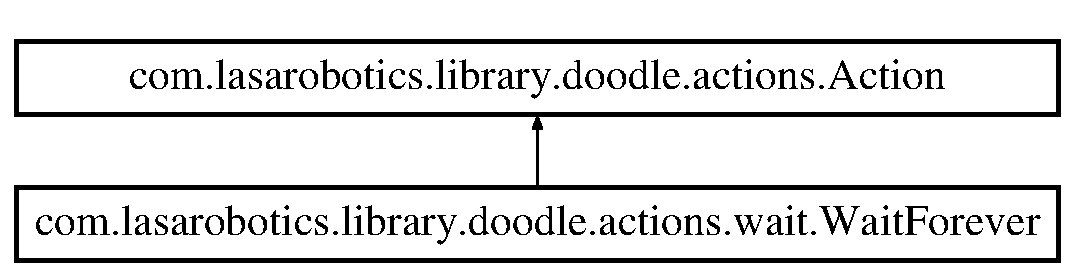
\includegraphics[height=2.000000cm]{classcom_1_1lasarobotics_1_1library_1_1doodle_1_1actions_1_1wait_1_1_wait_forever}
\end{center}
\end{figure}
\subsection*{Public Member Functions}
\begin{DoxyCompactItemize}
\item 
\hypertarget{classcom_1_1lasarobotics_1_1library_1_1doodle_1_1actions_1_1wait_1_1_wait_forever_a3bc44df6aeb098931a3034e8bdc0bee8}{}void {\bfseries run} (\hyperlink{classcom_1_1lasarobotics_1_1library_1_1doodle_1_1_doodle_run_data}{Doodle\+Run\+Data} data)\label{classcom_1_1lasarobotics_1_1library_1_1doodle_1_1actions_1_1wait_1_1_wait_forever_a3bc44df6aeb098931a3034e8bdc0bee8}

\item 
\hypertarget{classcom_1_1lasarobotics_1_1library_1_1doodle_1_1actions_1_1wait_1_1_wait_forever_acafd79d95cf4267b1948cb029b70f9a3}{}String {\bfseries to\+String} ()\label{classcom_1_1lasarobotics_1_1library_1_1doodle_1_1actions_1_1wait_1_1_wait_forever_acafd79d95cf4267b1948cb029b70f9a3}

\end{DoxyCompactItemize}
\subsection*{Additional Inherited Members}


\subsection{Detailed Description}
Waits a certain period of time 

The documentation for this class was generated from the following file\+:\begin{DoxyCompactItemize}
\item 
ftc-\/library/src/main/java/com/lasarobotics/library/doodle/actions/wait/Wait\+Forever.\+java\end{DoxyCompactItemize}

\hypertarget{classcom_1_1lasarobotics_1_1library_1_1doodle_1_1actions_1_1wait_1_1_wait_time}{}\section{com.\+lasarobotics.\+library.\+doodle.\+actions.\+wait.\+Wait\+Time Class Reference}
\label{classcom_1_1lasarobotics_1_1library_1_1doodle_1_1actions_1_1wait_1_1_wait_time}\index{com.\+lasarobotics.\+library.\+doodle.\+actions.\+wait.\+Wait\+Time@{com.\+lasarobotics.\+library.\+doodle.\+actions.\+wait.\+Wait\+Time}}
Inheritance diagram for com.\+lasarobotics.\+library.\+doodle.\+actions.\+wait.\+Wait\+Time\+:\begin{figure}[H]
\begin{center}
\leavevmode
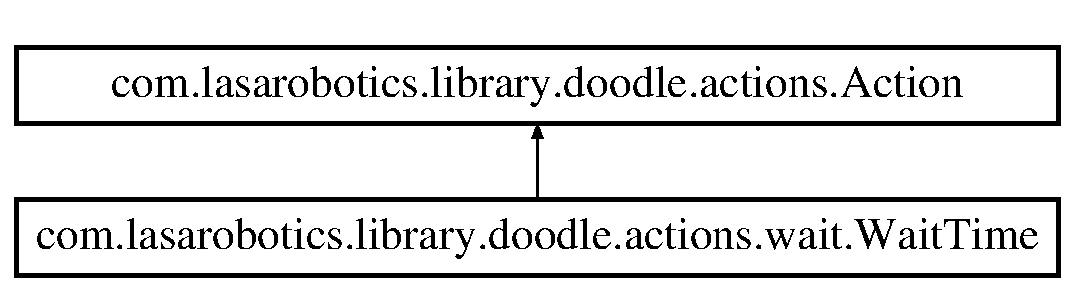
\includegraphics[height=2.000000cm]{classcom_1_1lasarobotics_1_1library_1_1doodle_1_1actions_1_1wait_1_1_wait_time}
\end{center}
\end{figure}
\subsection*{Public Member Functions}
\begin{DoxyCompactItemize}
\item 
\hypertarget{classcom_1_1lasarobotics_1_1library_1_1doodle_1_1actions_1_1wait_1_1_wait_time_affb23c52be0db8a44e12fedb0aea89b2}{}{\bfseries Wait\+Time} (long ms)\label{classcom_1_1lasarobotics_1_1library_1_1doodle_1_1actions_1_1wait_1_1_wait_time_affb23c52be0db8a44e12fedb0aea89b2}

\item 
\hypertarget{classcom_1_1lasarobotics_1_1library_1_1doodle_1_1actions_1_1wait_1_1_wait_time_aea50c785fa5f5f55d1d274173f858f39}{}void {\bfseries run} (\hyperlink{classcom_1_1lasarobotics_1_1library_1_1doodle_1_1_doodle_run_data}{Doodle\+Run\+Data} data)\label{classcom_1_1lasarobotics_1_1library_1_1doodle_1_1actions_1_1wait_1_1_wait_time_aea50c785fa5f5f55d1d274173f858f39}

\item 
\hypertarget{classcom_1_1lasarobotics_1_1library_1_1doodle_1_1actions_1_1wait_1_1_wait_time_a9705fce43d879bb2e04661934a3b2bda}{}String {\bfseries to\+String} ()\label{classcom_1_1lasarobotics_1_1library_1_1doodle_1_1actions_1_1wait_1_1_wait_time_a9705fce43d879bb2e04661934a3b2bda}

\end{DoxyCompactItemize}
\subsection*{Additional Inherited Members}


\subsection{Detailed Description}
Waits a certain period of time 

The documentation for this class was generated from the following file\+:\begin{DoxyCompactItemize}
\item 
ftc-\/library/src/main/java/com/lasarobotics/library/doodle/actions/wait/Wait\+Time.\+java\end{DoxyCompactItemize}

%--- End generated contents ---

% Index
\backmatter
\newpage
\phantomsection
\clearemptydoublepage
\addcontentsline{toc}{chapter}{Index}
\printindex

\end{document}
